\documentclass[12pt, a4paper]{article}
\usepackage[utf8]{inputenc}
\usepackage{hyperref, graphicx}
\usepackage[left=1.00in, right=1.00in, top=1.00in, bottom=1.00in]{geometry}
\title{CS348 Project Milestone 1}
\author{Keshav Gupta\and Isshana Mohanakumar \and Edward Pei \and Ricky Lu \and Govind Nair}

\begin{document}
\maketitle
\graphicspath{{./images/}}

\section*{R1. Application High-Level Description}
\label{sec:R1}
\subsection*{Description}
Our group is creating a web application that will allow University of Waterloo students to manage their undergraduate career. The application will allow users to track things such as the courses they have taken each term, as well as their final grades, their current course schedules, and their friends in the university. They will be able to visualize all the courses they've taken, their estimated GPA, and the courses that they share with their friends.\\

What sets us apart from other University applications like RateMyProf and UWFlow is that rather than focusing on individual courses, we consider the student's entire university career. We do this by calculating GPA's, persisting data from previous terms, and including this data in future analysis. We also help them plan courses based on pre-requisites and the courses their friends are taking. We will be a tool that the students use during their entire degree.

\subsection*{Dataset Source}
We will use the \underline{\href{https://openapi.data.uwaterloo.ca/api-docs/index.html}{University of Waterloo Open Data API}} to download the department, courses, and term data. The API responses provided by the Open Data API will be provided in a JSON format, so we will need to process it into our MySQL tables.\\

The dataset processing can be seen in \underline{\hyperref[sec:R3]{R3}} for the sample dataset, and \underline{\hyperref[sec:R4]{R4}} for the production dataset.

\subsection*{Our Users}
Our target demographic is University of Waterloo students who want to keep track of the courses they have taken, their grades, and manage their degree requirements.\\

They are the people who don't particularly like the native bare-bones HTML page that the university provides. Our users are the students who want something more involved so that they don't spend so much time browsing the undergraduate calendar to plan their next term of courses.

\subsection*{Administrators}
The administrators of our application will be the group members as specified at the top of this document. Administrators will have command-line access to the MySQL data base. The rest of the users will have basic student level access to the below proposed features, meaning that they can only interact with the feature as defined in the feature descriptions.

\subsection*{Features}
Below are the features of our application. You can click on them to view the feature description.
\subsubsection*{Basic Features}
\begin{itemize}
    \item \hyperref[sec:R6]{R6. User registration, login, and management}
    \item \hyperref[sec:R7]{R7. List, search, add, and delete courses}
    \item \hyperref[sec:R8]{R8. Add user's student schedule}
    \item \hyperref[sec:R9]{R9. Manage friends (other students), and view friends that are taking the same courses and lectures as the user}
    \item \hyperref[sec:R10]{R10. Add previous courses taken as well as your final grades to calculate GPA}
    \item \hyperref[sec:R11]{R11. Show all courses you can take based on pre-requisites and anti-requisites}
\end{itemize}

\subsubsection*{Fancy Features}
\begin{itemize}
    \item \hyperref[sec:R12]{R12. Pre-requisite graphs for a given course}
    \item \hyperref[sec:R13]{R13. AI Model that suggests courses to users based on the courses they already took}
    \item \hyperref[sec:R14]{R14. Update detailed course grades such as individual assignments, midterms, and exams to estimate final course grade}
    \item \hyperref[sec:R15]{R15. SQL injection protection by sanitizing queries and password hashing}
    \item \hyperref[sec:R16]{R16. Enter your course deadlines and receive emails when the deadline is approaching}
\end{itemize}
\subsubsection*{Changes In This Report}
I was unable to find out how to properly change text color in latex, below is a full list of everything major that was changed in this report.
\begin{itemize}
    \item RXc for all features.
    \item RXd for \underline{\hyperref[sec:R6]{R6}}, \underline{\hyperref[sec:R7]{R7}}, and \underline{\hyperref[sec:R8]{R8}}.
    \item Updated production algorithm notes.
    \item Implemented endpoints for back-end of some features (see README current features).
    \item Implemented UI for front-end of some features (see README current features).
    \item Added content to README.
    \item Added C4 information.
    \item Added Create Indexes link to C2.
    \item Updated READMEs for front-end and back-end startup.
\end{itemize}
\section*{R2. System Support Description}
\label{sec:R2}

Our front-end interface will be a web application built in React. Our back-end API server will be built with Node.js and Express.js. These will rely on a MySQL database. Generally, our entire tech stack will be built with either JavaScript or TypeScript with SQL queries to interact with the database. We also expect to use JavaScript to process JSON data from the \href{https://openapi.data.uwaterloo.ca/api-docs/index.html}{University of Waterloo Open Data API} into our MySQL database.\\

All of this will need to be run locally and requires \href{https://nodejs.org/en/download}{Node v18.5.0}, \href{https://nodejs.org/en/download}{NPM v8.12.1}, \href{https://dev.mysql.com/downloads/mysql/}{MySQL v8.0.33}. The application may work for other versions, but we will be developing and testing it using the ones specified above.\\

Since all of the above technologies are supported on all major operating systems such as MacOS, Linux, and Windows, it can be run locally on any of these three systems. It might support more systems, but these are the main three that the majority of the world uses, which is why we specifically name these ones.

\section*{R3. Database With Sample Dataset}
\label{sec:R3}

\subsubsection*{Populating Data}
A step-by-step guide on how to use the script to populate the database is available on the \underline{\href{https://github.com/Kggupta/DegreeMap/blob/main/README.md}{GitHub Repository}}.\\
\textbf{Basic directions:}
\begin{itemize}
    \item Open a command prompt
    \item Navigate to the directory with \underline{cd DegreeMap/Database}
    \item Fill the \textbf{.env} file with the relevant data. The required fields are highlighted in the \underline{\href{https://github.com/Kggupta/DegreeMap/blob/main/README.md}{README}}.
    \item \href{https://nodejs.org/en/download}{Install Node and NPM} if you haven't already. This is very simple and just requires clicking confirm once the installation is complete.
    \item Install the NPM dependencies with \underline{npm install}
    \item Run the script with
    \underline{node PopulateData.js sample}
\end{itemize}
\subsubsection*{How The Data Is Generated/Cleaned/etc.}
The sample data is hard-coded in CSV files under \underline{\href{https://github.com/Kggupta/DegreeMap/tree/main/Database/DataFiles/Sample}{Database/DataFiles/Sample/}}\\

First, all the tables in the database are dropped using the \underline{\href{https://github.com/Kggupta/DegreeMap/tree/main/Database/Queries}{DropTables.sql}} file, removing all configuration and data that already exists. Then, the tables and triggers are re-defined with no values using the \underline{\href{https://github.com/Kggupta/DegreeMap/tree/main/Database/Queries}{CreateTables.sql}} file. The triggers are also added with \underline{\href{https://github.com/Kggupta/DegreeMap/tree/main/Database/Queries}{CreateTriggers.sql}}. Then, the script determines whether the user specified \textbf{sample} or \textbf{prod} in the command arguments. If \textbf{sample} was selected, then the script iterates over each CSV file, using it's file name as the table name to insert into, and the header list of attributes as the table's property names. The script goes in a specific order that's specified in the \underline{\href{https://github.com/Kggupta/DegreeMap/blob/main/Database/InsertionOrder.json}{InsertionOrder.json}} file, to ensure that the foreign key constraints aren't violated at any point of the script. For each CSV file, it iterates over the rows of the CSV file by separating it by end-lines, inserting each sequentially.
\subsubsection*{Data Description}
Below is some statistics about what the sample data contains.
\begin{center}
    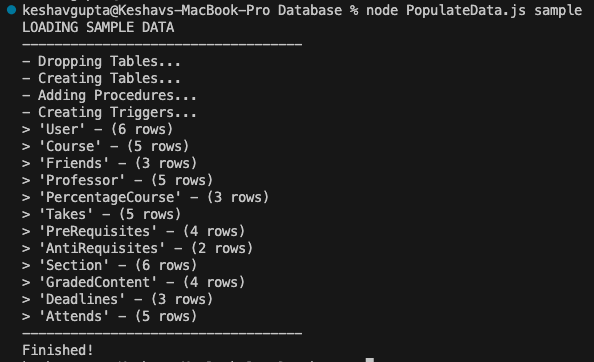
\includegraphics[width=\textwidth]{sampledata}
\end{center}

This sample data contains 5 administrator users (the group members) as well as one regular dummy user. It has 5 unique courses (CS348, CS449, CS492, HRM200, CLAS104), 5 professors, friendships between the administrator users. It also has pre-requisites between CS348, CS492, and CS449. There is also an anti-requisite between HRM200 and CLAS104, as well as the reverse of the pre-requisite between CS348 and CS492. Meaning that if a student takes CS492, they can't take CS348 anymore.\\
Student 1 (Keshav) is entered as taking CS348, CLAS104, and CS449. Student 2 (Isshana) is taking HRM200, CS492, and CS348.\\

The course schedule dates are designed to overlap in different ways to demonstrate the features we describe later in the report. All courses except HRM and CLAS are percentage graded courses.
\section*{R4. Database With Production Dataset}
\label{sec:R4}
\subsubsection*{Description of The Data}
This data is the production dataset and contains all the course, instructor, section, schedule, etc. data for the most recent term of the university. It also includes courses that aren't offered this term. There is 6 users, the same as the sample data. The abilities of the administrator are described later in the report.\\

Below is an image of what this database looks like. Tables that are not in this list have 0 rows since they all depend on users actually adding to them through the features we describe in later sections.
\begin{center}
    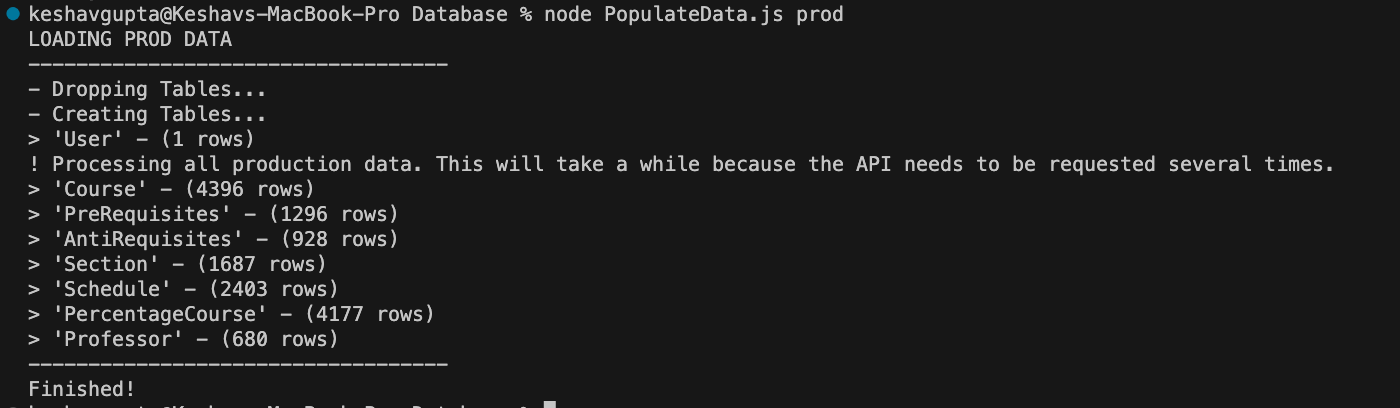
\includegraphics[width=\textwidth]{proddata}
\end{center}
\subsubsection*{Generating/Populating/Cleaning/Importing The Database}
This data is the production dataset. It's generated from the \href{https://openapi.data.uwaterloo.ca/api-docs/index.html}{University of Waterloo Open Data API}.\\

The script usage is identical to the sample database, except that the user supplies \textbf{prod} instead of \textbf{sample} as the command-line argument. The usage guide has not been re-described here to avoid repetition.\\

The API Token is required to run this script, which you can get by using the \href{https://openapi.data.uwaterloo.ca/api-docs/index.html}{University of Waterloo Open Data API} and follow their steps. The Token will be emailed to you.\\

Once you run the script as described above, it operates as follows to generate, populate, clean and import the production data into the database:
\begin{itemize}
    \item Drop all existing tables in the database using \underline{\href{https://github.com/Kggupta/DegreeMap/blob/main/Database/Queries/DropTables.sql}{DropTables.sql}} by leveraging the mysql2 npm library to create a connection to the local database and running the sql script.
    \item Create all tables in the database along with their contraints, triggers, indexes, etc using the \underline{\href{https://github.com/Kggupta/DegreeMap/blob/main/Database/Queries}{queries}}.
    \item Enters the module that populates the production data using \underline{\href{https://github.com/Kggupta/DegreeMap/blob/main/Database/src/PopulateProductionData.js}{PopulateProductionData.js}}.
    \item Insert the administrator user in the database, which is stored as a CSV file in the production \underline{\href{https://github.com/Kggupta/DegreeMap/blob/main/Database/DataFiles/Prod/User.csv}{User.csv}}.
    \item Send a get request to the University API to query the most recent term using \href{https://openapi.data.uwaterloo.ca/v3/Terms/current}{GET: api/v3/Terms/current}
    \item Get all courses using the current term code that we retrieved through the API using \href{https://openapi.data.uwaterloo.ca/v3/Courses/1235}{GET: api/v3/Courses/term}
    \item Iterate over every course in the response, first inserting each course using the INSERT command.
    \item If the \textbf{gradingBasis} property is \underline{NUM}, add the course ID to the PercentageCourse database as well.
    \item Now, using RegEx, it cleans the course requirements string and finds the keywords 'Prereq' and 'Antireq'. Further cleaning is done by matching ([A-Z]+ ?[0-9]+)+, separated by commas. It gets the courses which are specified after the keyword. Then, stores the value in a temporary variable until all courses are finished inserting to avoid Foreign key constraint issues.
    \item Next, the API is requested again, this time the \href{https://openapi.data.uwaterloo.ca/v3/CourseSchedules/term/subject/coursenumber}{GET: api/v3/CourseSchedules/term/CS/348} endpoint. The URL is filled as an example.
    \item Once this data is retrieved, it iterates through each section in the response.
    \item While iterating, it adds professors to the Professor table if they haven't already been added.
    \item During the iteration, it then adds the section to the Section database, along with the scheduled timing.
    \item To allow for bitwise operators of weekly section offering pattern codes, the script converts the (Y|N) 7 character length string into an integer. The integer maps to whatever the 7 digit binary would be. For example, \textbf{YYYNNNN} translates to \textbf{1110000}, then it's \textbf{112} in decimal.
    \item The data is cleaned in this step to handle cases when there's no instructor assigned to the course or no location by assigning NULL. It also makes sure the given date pattern is valid.
    \item Finally, once the section and course loops are complete, the pre/anti-requisites are added to their respective tables.
    \item The number of added rows is printed to the console and the script ends.
\end{itemize}
\section*{R5. Schema Design}
\label{sec:R5}

\subsection*{R5a. Assumptions}
We made a few assumptions for this project database. We also included some general specifications, so there are a couple extra things we specify here that aren't assumptions, but are still important to the application.\\
\textbf{General Notes:} 
\begin{itemize}
    \item Mentions of \underline{course ID} is equivalent to the combination of \underline{course subject} and \underline{course number}. Example: CS348
    \item Academic level, or simply "level" in the database, references the terminology of 1A to 4B. This is XY, where X is the year number [1,2,3,4] and Y is the term number [A,B].
\end{itemize}
\textbf{Users}
\begin{itemize}
    \item User ID is unique to users.
    \item A user is either a regular user or an application administrator.
    \item User is an undergraduate student so their 'level' is within 1A to 4B.
    \item User can be friends with as many other users as they want. But, they cannot be friends with themselves.
\end{itemize}
\textbf{Courses}
\begin{itemize}
    \item Course ID is unique to courses. For example, CS348 only represents Introduction to Databases and nothing else.
    \item Some courses are not offered in a particular term, so they have no associated sections.
    \item Courses can have any number of pre-requisites and anti-requisites.
    \item Pre/Anti-requisites are other Course IDs.
    \item Courses can't be pre/anti requisites of themselves. This cannot be shown in the E/R diagram, but it is still an assumption.
    \item If a user takes any pre-requisite of a course, they can take that course, unless they have already taken an anti-requisite of the course.
    \item If a user has taken any anti-requisite of a course, they cannot take that course, even if they took a pre-requisite for it.
    \item Courses can't be both a pre-requisite and an anti-requisite of the same course.
    \item A user can take 0 or more unique courses.
    \item Users cannot take the same course twice in their undergraduate career.
    \item Courses are graded on a percentage or credit received basis.
    \item When a user takes a course that is graded on a percentage basis during some level (1A to 4B), they receive a grade within [0, 100] for the course.
    \item When a user takes a course that is graded on a credit received basis during some level (1A to 4B), they receive a NULL grade for the course.
\end{itemize}
\textbf{Professors}
\begin{itemize}
    \item Professor uid uniquely identifies professors.
    \item Professors have a name attribute.
    \item It's possible for a professor to teach 0 courses.
    \item A professor can teach as many things as they want.
    \item A professor can't teach two timings of a section that happen at the same day and time. This cannot be shown by the E/R diagram, but it's still an assumption.
\end{itemize}
\textbf{Sections}
\begin{itemize}
    \item A course section is uniquely identified by the section code, and the course ID (subject + course code) all combined.
    \item Users can attend up to 15 sections at once.
    \item Users might attend 0 course sections, but still be taking/have taken courses.
    \item Users cannot attend two sections that are scheduled during the same day and time.
    \item A section has a single timing schedule.
    \item A location is defined by it's room and building names.
    \item The days that a section timing can be offered are Monday to Sunday.
    \item Sections timings can occur on multiple days in a week.
    \item A section type can be a Lecture (LEC), Tutorial (TUT), Test (TST), etc.
    \item Sections must be associated to one course.
    \item Sections of a course can be attended by 0 or more people.
    \item A single section is taught by zero or one professor.
\end{itemize}
\textbf{Deadlines}
\begin{itemize}
    \item Deadlines are items that denote when something like an assignment is due.
    \item Deadlines for a course are uniquely identifiable using the combined user ID who added the deadline, the course ID and the deadline name.
    \item Deadlines are due at some date in the future, within the next four months of when it was added.
    \item A course or user may have no deadlines, but deadlines must be assigned to a course and user.
    \item Both percentage and credit received courses can have deadlines.
\end{itemize}
\textbf{Graded Content}
\begin{itemize}
    \item Graded content are assignments, midterms, exams, etc.
    \item Graded content for a course is uniquely identifiable using the combined user ID who completed the content, the course ID, and the name of the content.
    \item Graded content has a name, a grade out of 100, and a weight out of 100.
    \item The sum of the weights of all the graded content for a specific course must be greater than or equal to 0 and less than or equal to 100. This cannot be shown in the E/R diagram, but it is still an assumption.
    \item The grade out of 100 might be greater than 100 because of bonus marks.
    \item Grades and weights cannot be less than 0. This cannot be shown in the E/R diagram, but it is still an assumption.
    \item A course or user may have no graded content, but any graded content must be assigned to a course and user.
    \item Only courses with a percentage grading basis can have graded content.
\end{itemize}

\subsection*{R5b. E/R Diagram}
\begin{center}
    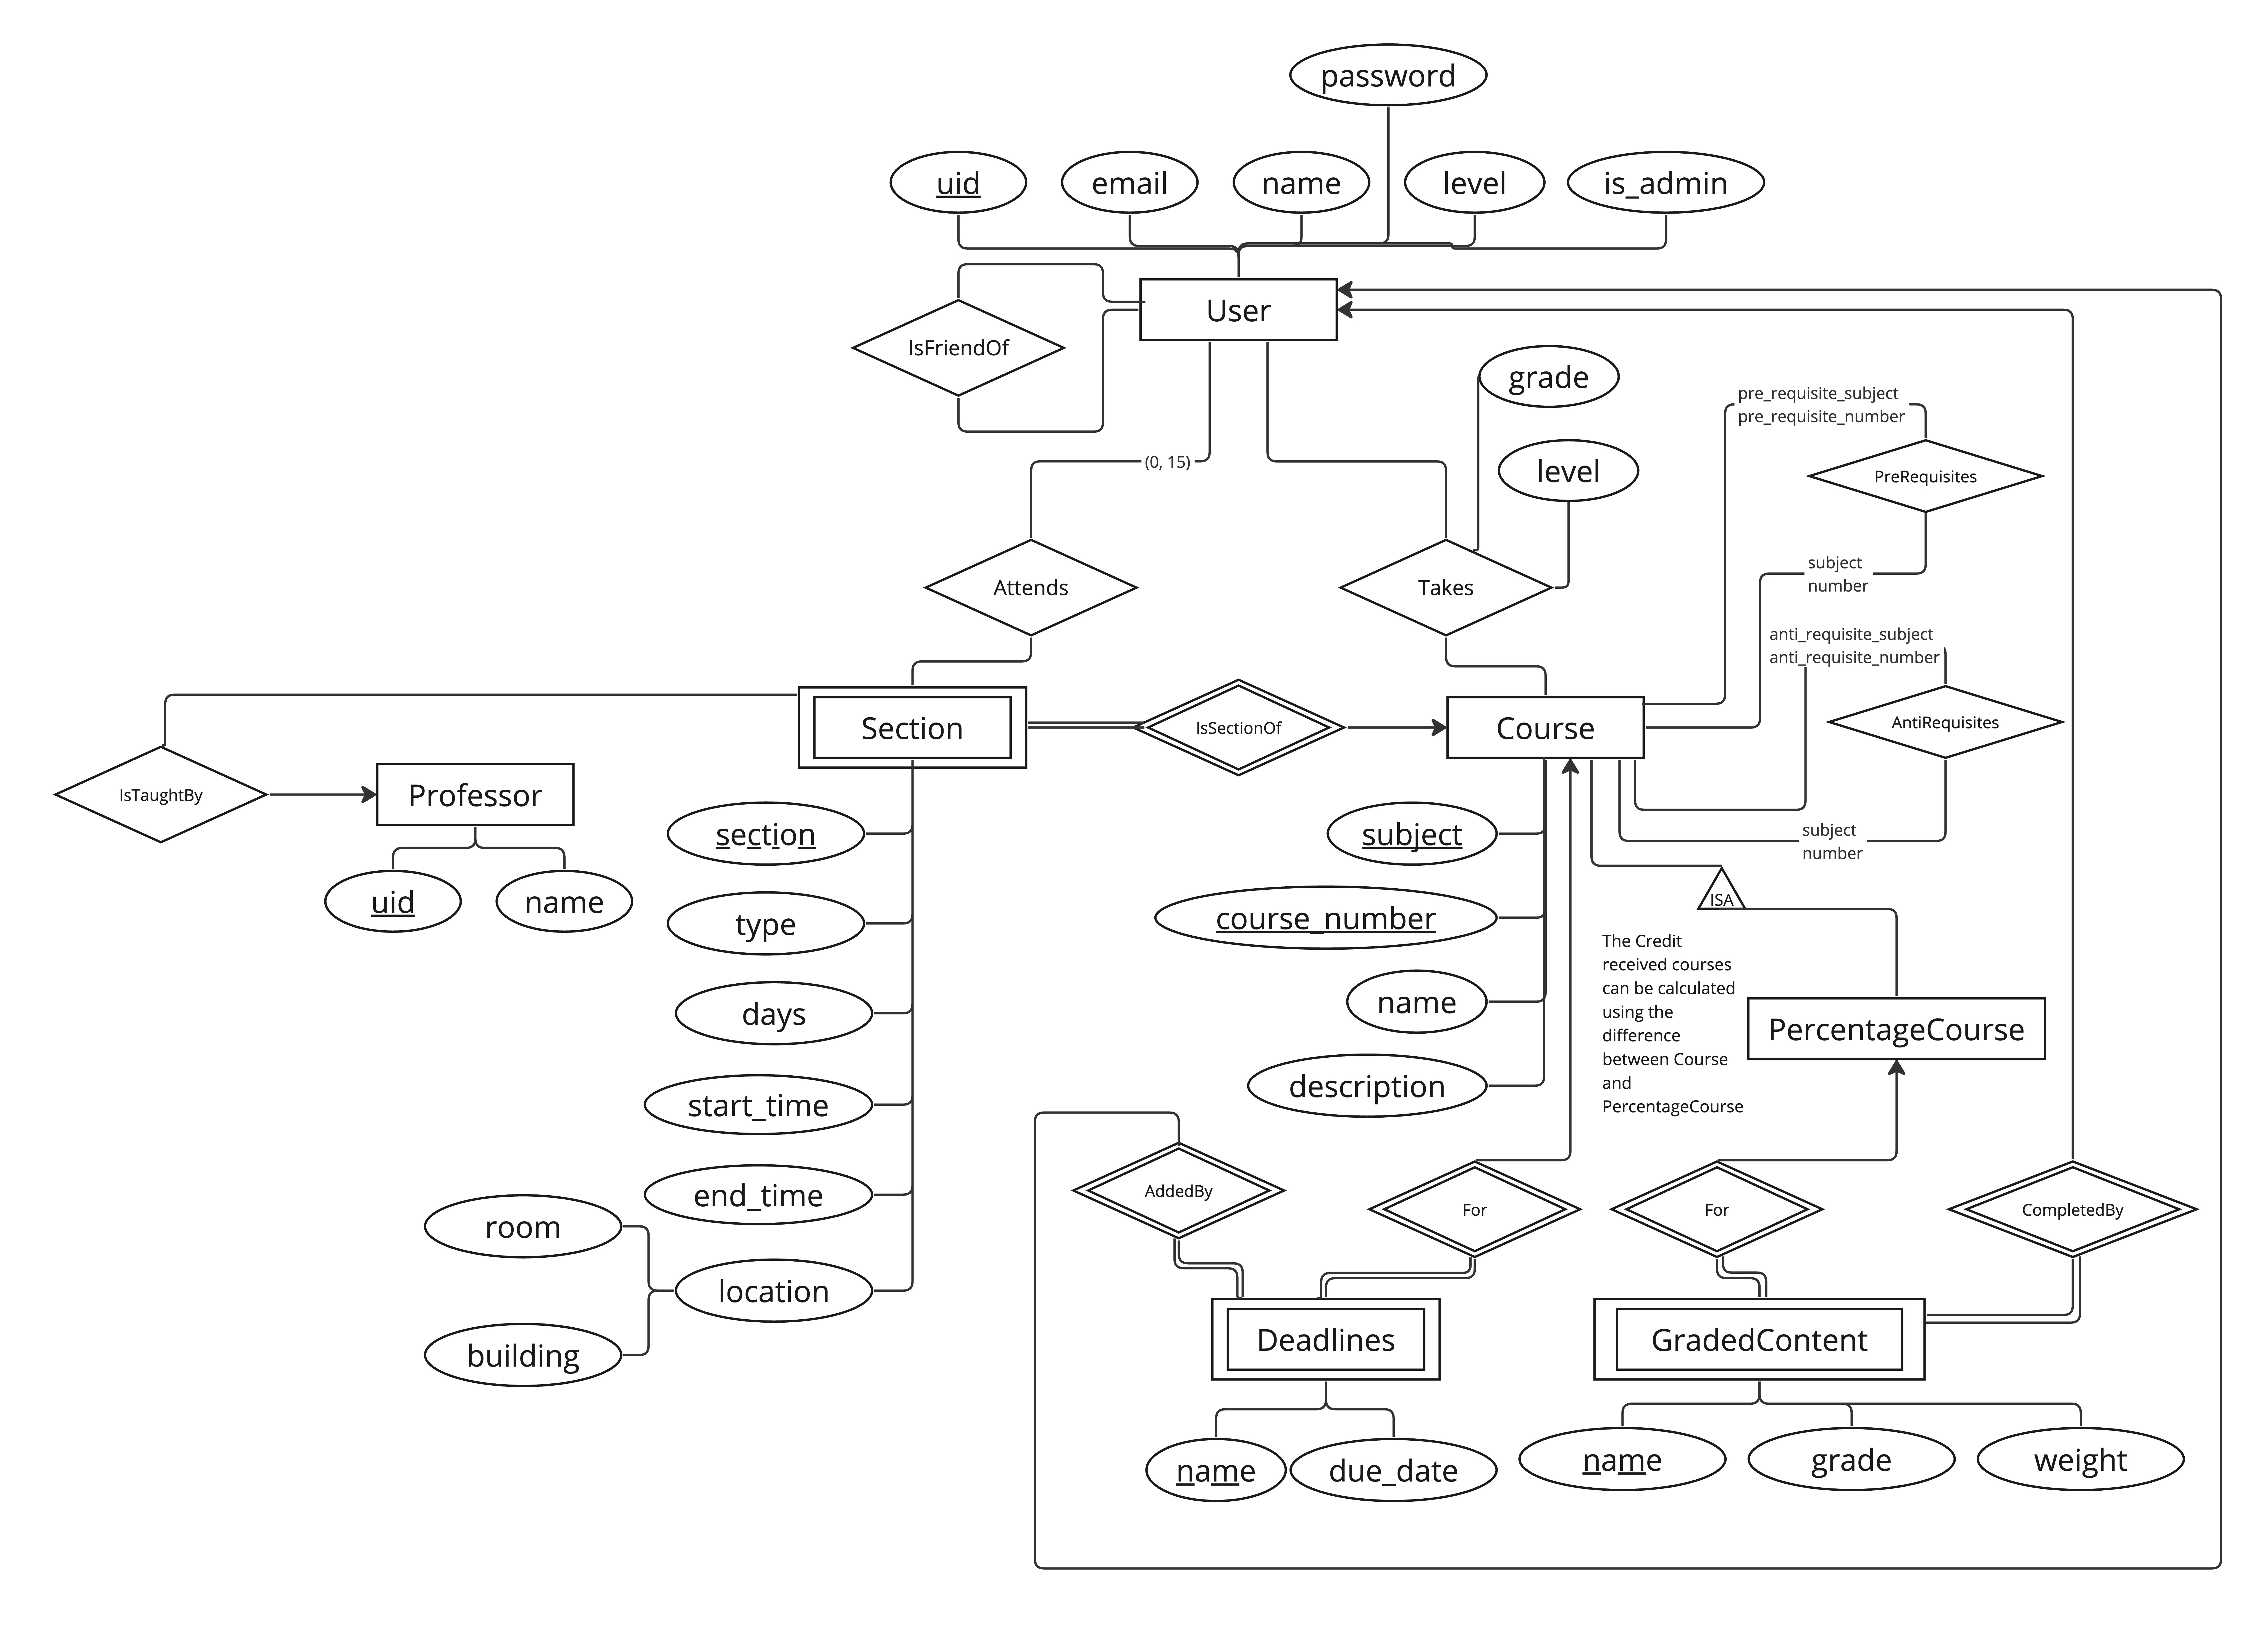
\includegraphics[width=\textwidth]{erd}
\end{center}
If the image is too compressed to see clearly, you can view the \underline{\href{https://miro.com/app/board/uXjVM-yog60=/}{Miro board}}.\\

\textbf{Password:} cs348course
\subsection*{R5c. Relational Data Model}
- \textbf{User}(\underline{uid}, email, name, password, level, is\_admin)\\
- \textbf{Course}(\underline{subject}, \underline{course\_number}, name, description)\\
- \textbf{Professor}(\underline{uid}, name)\\
- \textbf{PercentageCourse}(\underline{subject}, \underline{course\_number})\\
FK: (subject, course\_number) references Course\\
- \textbf{PreRequisites}(\underline{subject}, \underline{course\_number}, \underline{pre\_requisite\_subject}, \underline{pre\_requisite\_number})\\
FK: (subject, course\_number) references Course\\
FK: (pre\_requisite\_subject, pre\_requisite\_number) references Course\\
- \textbf{AntiRequisites}(\underline{subject}, \underline{course\_number}, \underline{anti\_requisite\_subject}, \underline{anti\_requisite\_number})\\
FK: (subject, course\_number) references Course\\
FK: (anti\_requisite\_subject, anti\_requisite\_number) references Course\\
- \textbf{Section}(\underline{section}, \underline{subject}, \underline{course\_number}, type, professor\_id, days, start\_time, end\_time, location\_room, location\_building)\\
FK: (subject, course\_number) references Course\\
FK: professor\_id references Professor\\
- \textbf{Takes}(\underline{uid}, \underline{subject}, \underline{course\_number}, grade, level)\\
FK: uid references User\\
FK: (subject, course\_number) references Course\\
- \textbf{Attends}(\underline{uid}, \underline{section}, \underline{subject}, \underline{course\_number})\\
FK: uid references User\\
FK: (section, subject, course\_number) references Section\\
- \textbf{Friends}(\underline{uid1}, \underline{uid2})\\
FK: uid1 references User\\
FK: uid2 references User\\
- \textbf{Deadlines}(\underline{uid}, \underline{subject}, \underline{course\_number}, \underline{name}, due\_date)\\
FK: uid references User\\
FK: (subject, course\_number) references Course\\
- \textbf{GradedContent}(\underline{uid}, \underline{subject}, \underline{course\_number}, \underline{name}, grade, weight)\\
FK: uid references User\\
FK: (subject, course\_number) references PercentageCourse\\

\section*{R6. User Registration, Login, and Management}
\label{sec:R6}
\subsection*{R6a. Interface Design}
\subsubsection*{User Registration}
The user, which is the UW student population in this case, is able to enter their email, full name, password, and academic level to register for the website. There will be text boxes for email, full name, and academic level. There will be a password box with hidden asterix text when text is entered to record the password. The full name must be within 1 and 50 alphanumeric characters. The academic level must be two characters, the first being the integer year that the student is currently studying, and the second is A or B depending on whether they are in their first or second term of that year. The year is within 1 and 4. The password is a 8 to 25 character ASCII string and both the password and the confirmation must be the same. All fields are required. When the user hits the register button, it will insert their user details into the User table, and go to the main page of the application. If any of the requirements of the text fields are violated, the application will keep the register button disabled. If the user email has already been registered, the application will show an error box when the user presses register and prompt them to login instead.
\subsubsection*{User Authentication}
Another related feature is that UW students (the user) is able to login to the application if they already have an account. The user enters their email (text box) and password (password box). If the email and password match an existing account, when the users presses login, it will take them to the home page of the application, with their account details filled in. If the email or password do not match, the application will show an error box and prompt them to try again instead of going to the home page.
\subsubsection*{Updating User Details}
UW Students are also able to update their academic level on the home page of the application once they are signed in. In the top area of the window, near the toolbar, the user can enter their new academic level and press confirm. The textbox will only allow valid academic levels to be typed. This means that if the user tries to type an invalid character that doesn't match the pattern, the character will not appear in the text box. The confirmation button will only update the academic level when the textbox is fully filled out. This is important because students are promoted to the next academic level every time they successfully complete a term, so this entry will be used so that their next courses will be added with the correct academic level.
\subsubsection*{Admin Functionalities}
App administrators have a section under the updating user details area that lists all the users in the application. In this view, they will be able to see the user ID's, names, and a promotion button for all the registered users along with a Delete button in the list. If the Delete is clicked, the row in the list will disappear and the user will be deleted, along with all of their information and references to them in the database. If the promote button for a specific user is clicked, it will updat ethe user to be an administrator in the database. Only users with the admin property set as true are considered app administrators, and would be able to see this view.
\subsection*{R6b. SQL Query, Testing With Sample Data}
The test sql file with all of these queries can be viewed here: \underline{\href{https://github.com/Kggupta/DegreeMap/tree/main/Database/Queries/TestSample}{TestSample/R6.sql}}, \underline{\href{https://github.com/Kggupta/DegreeMap/tree/main/Database/Queries/TestSample}{TestSample/R6.out}}. All SQL Queries are commented to explain what it does for this feature.

\begin{center}
    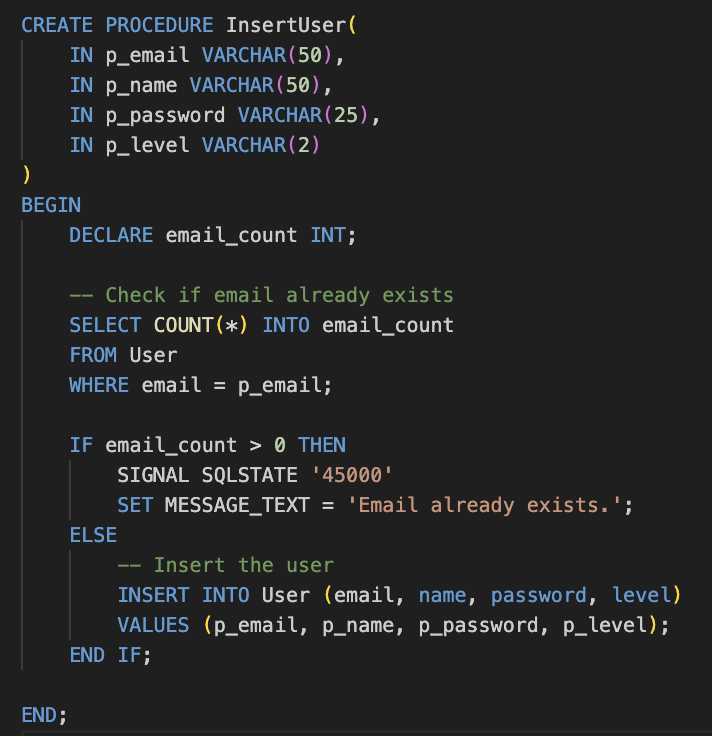
\includegraphics[width=250px]{R6/q1}
    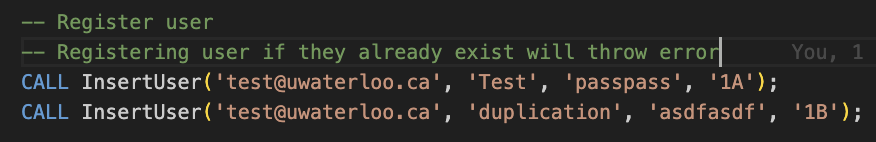
\includegraphics[width=250px]{R6/q1_1}
    \begin{verbatim}
Query OK, 1 row affected (0.00 sec)

ERROR 1644 (45000): Email already exists.
    \end{verbatim}
\end{center}
The above query adds a user to the database. It requires that the email doesn't already exist in the database. The application would insert the correct values in place of the sample ones shown in the image. Email is a possible candidate key, but we decided not to use it as the primary key for performance reasons, since comparing integers (uid) is likely faster than comparing strings (emails).
\begin{center}
    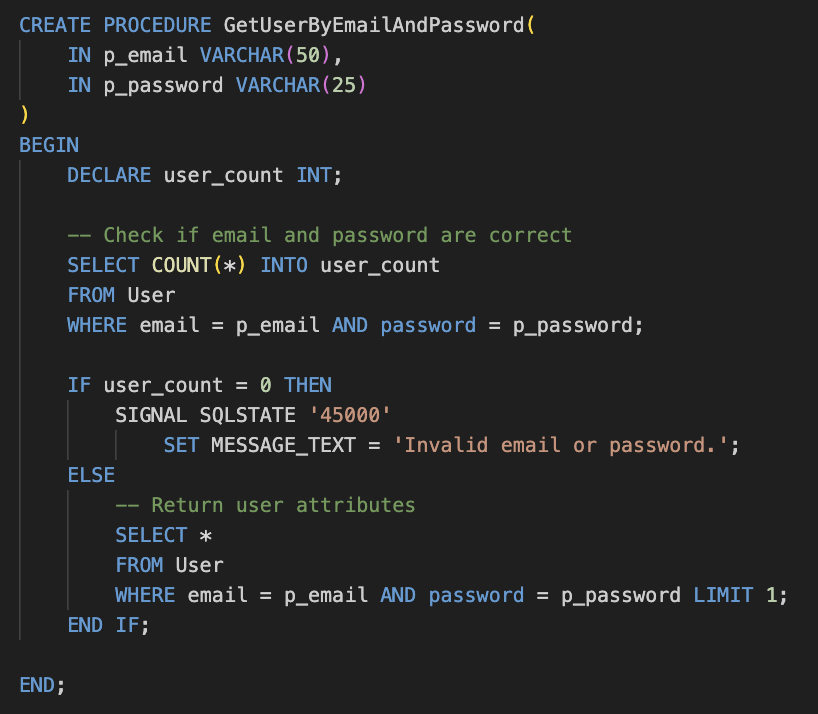
\includegraphics[width=400px]{R6/q2}
    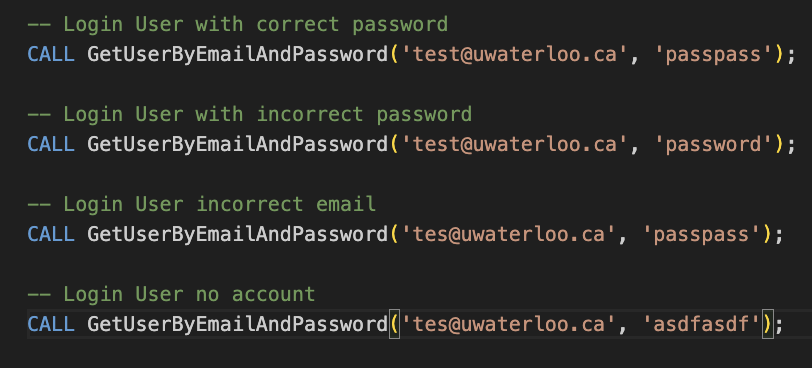
\includegraphics[width=400px]{R6/q2_1}
    \begin{verbatim}
+-----+-------------------+------+----------+-------+----------+
| uid | email             | name | password | level | is_admin |
+-----+-------------------+------+----------+-------+----------+
|   8 | test@uwaterloo.ca | Test | passpass | 1A    |        0 |
+-----+-------------------+------+----------+-------+----------+
1 row in set (0.00 sec)

Query OK, 0 rows affected (0.00 sec)

ERROR 1644 (45000): Invalid email or password.
ERROR 1644 (45000): Invalid email or password.
ERROR 1644 (45000): Invalid email or password.
    \end{verbatim}
\end{center}
The above query tests the various login cases with the test account that was inserted earlier. The first is when a user logs in with the correct email and password, then the user details will be returned. The following three cases show how when incorrect details are given, no user is found, so the login is invalid. 
\begin{center}
    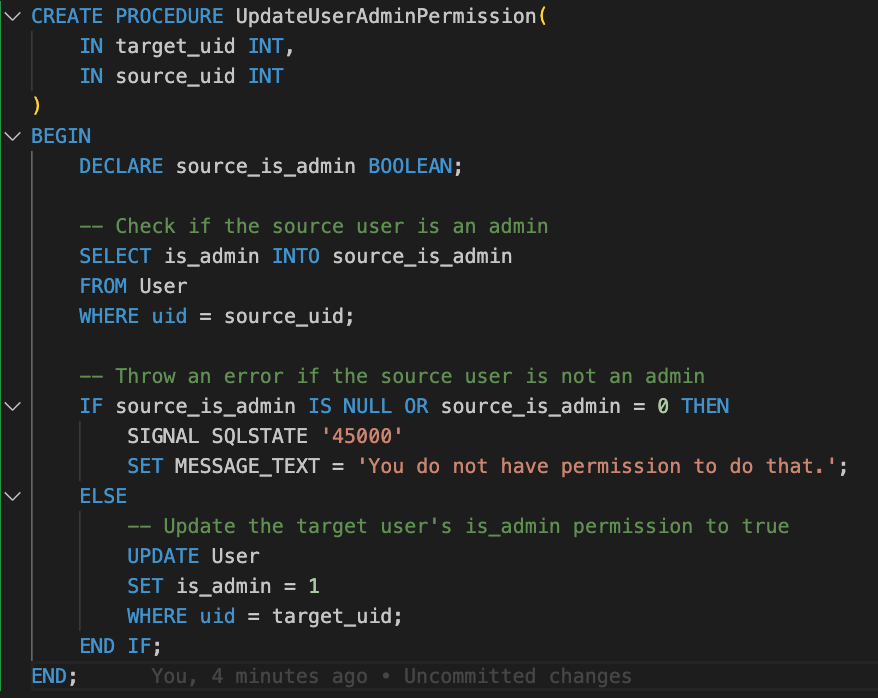
\includegraphics[width=400px]{R6/q3_2}
    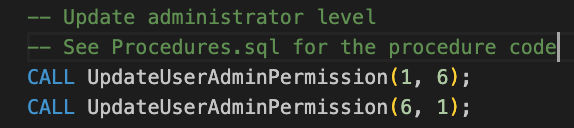
\includegraphics[width=400px]{R6/q3_1}
    \begin{verbatim}
ERROR 1644 (45000): You do not have permission to do that.
Query OK, 1 row affected (0.00 sec)
    \end{verbatim}
\end{center}
The above query updates a user to be an admin user. It first checks that the source user (the admin who is changing the permission) is actually an administrator, in the first case, user 6 is a standard account so they cannot change admin permissions, therefore, it throws a state 45000. The second query shows a successful case which is when the source user does have admin.

\begin{center}
    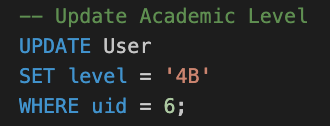
\includegraphics[width=400px]{R6/q4}
    \begin{verbatim}
Query OK, 1 row affected (0.01 sec)
Rows matched: 1  Changed: 1  Warnings: 0
    \end{verbatim}
\end{center}
This is just a simple query that is used to update the academic level of a user. The existence of the user would be an invariant that's set by the UI.

\subsection*{R6c. SQL Query, Testing With Production Data}
The test sql file with all of these queries can be viewed here: \underline{\href{https://github.com/Kggupta/DegreeMap/tree/main/Database/Queries/TestProduction}{TestProduction/R6.sql}}, \underline{\href{https://github.com/Kggupta/DegreeMap/tree/main/Database/Queries/TestProduction}{TestProduction/R6.out}}. All SQL queries are commented to explain what it does for this feature.

In this case, there are no optimizations to be made to the production queries. This is because most queries are occurring on the primary key, and by default MySQL treats the primary key as a dense index. Therefore, there is no improvements in terms of performance. 
We did however add the UNIQUE keyword to the email property in User, but not for the performance improvement since it's a negligible change and likely doesn't create any performance improvements. We verified this by adding ~2000 random users with different emails, then we performed several logins (one login procedure call is shown in R6.sql) with and without the UNIQUE keyword. From this, we confirmed that there was no noticeable change in performance time. We will however keep the change because it enforces the requirement that email is unique within the DBMS which is good for logical data integrity.
\begin{center}
    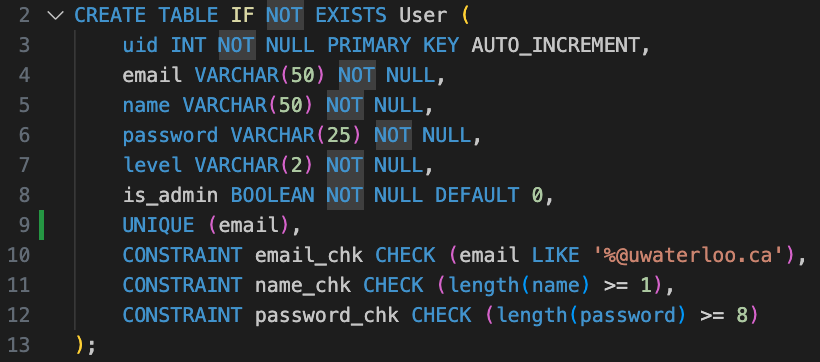
\includegraphics[width=400px]{R6/unique}
\end{center}
Additionally, searching by email and password only occur once during a user session during the login or registration, after that, the UID is used. Therefore, there are no performance improvements to be made here.
Since there was no change to the SQL queries themselves, we will not re-include them directly in the report.

\subsection*{R6d. Implementation, Snapshot, Testing}
Below are screenshots of the application showing login, registration, log out, account details updating, and user management for administrators (deleting users and promoting users to admins) in that order.
The code files are highlighted in the \textbf{Current Features} section of the README in the repository.
\begin{center}
        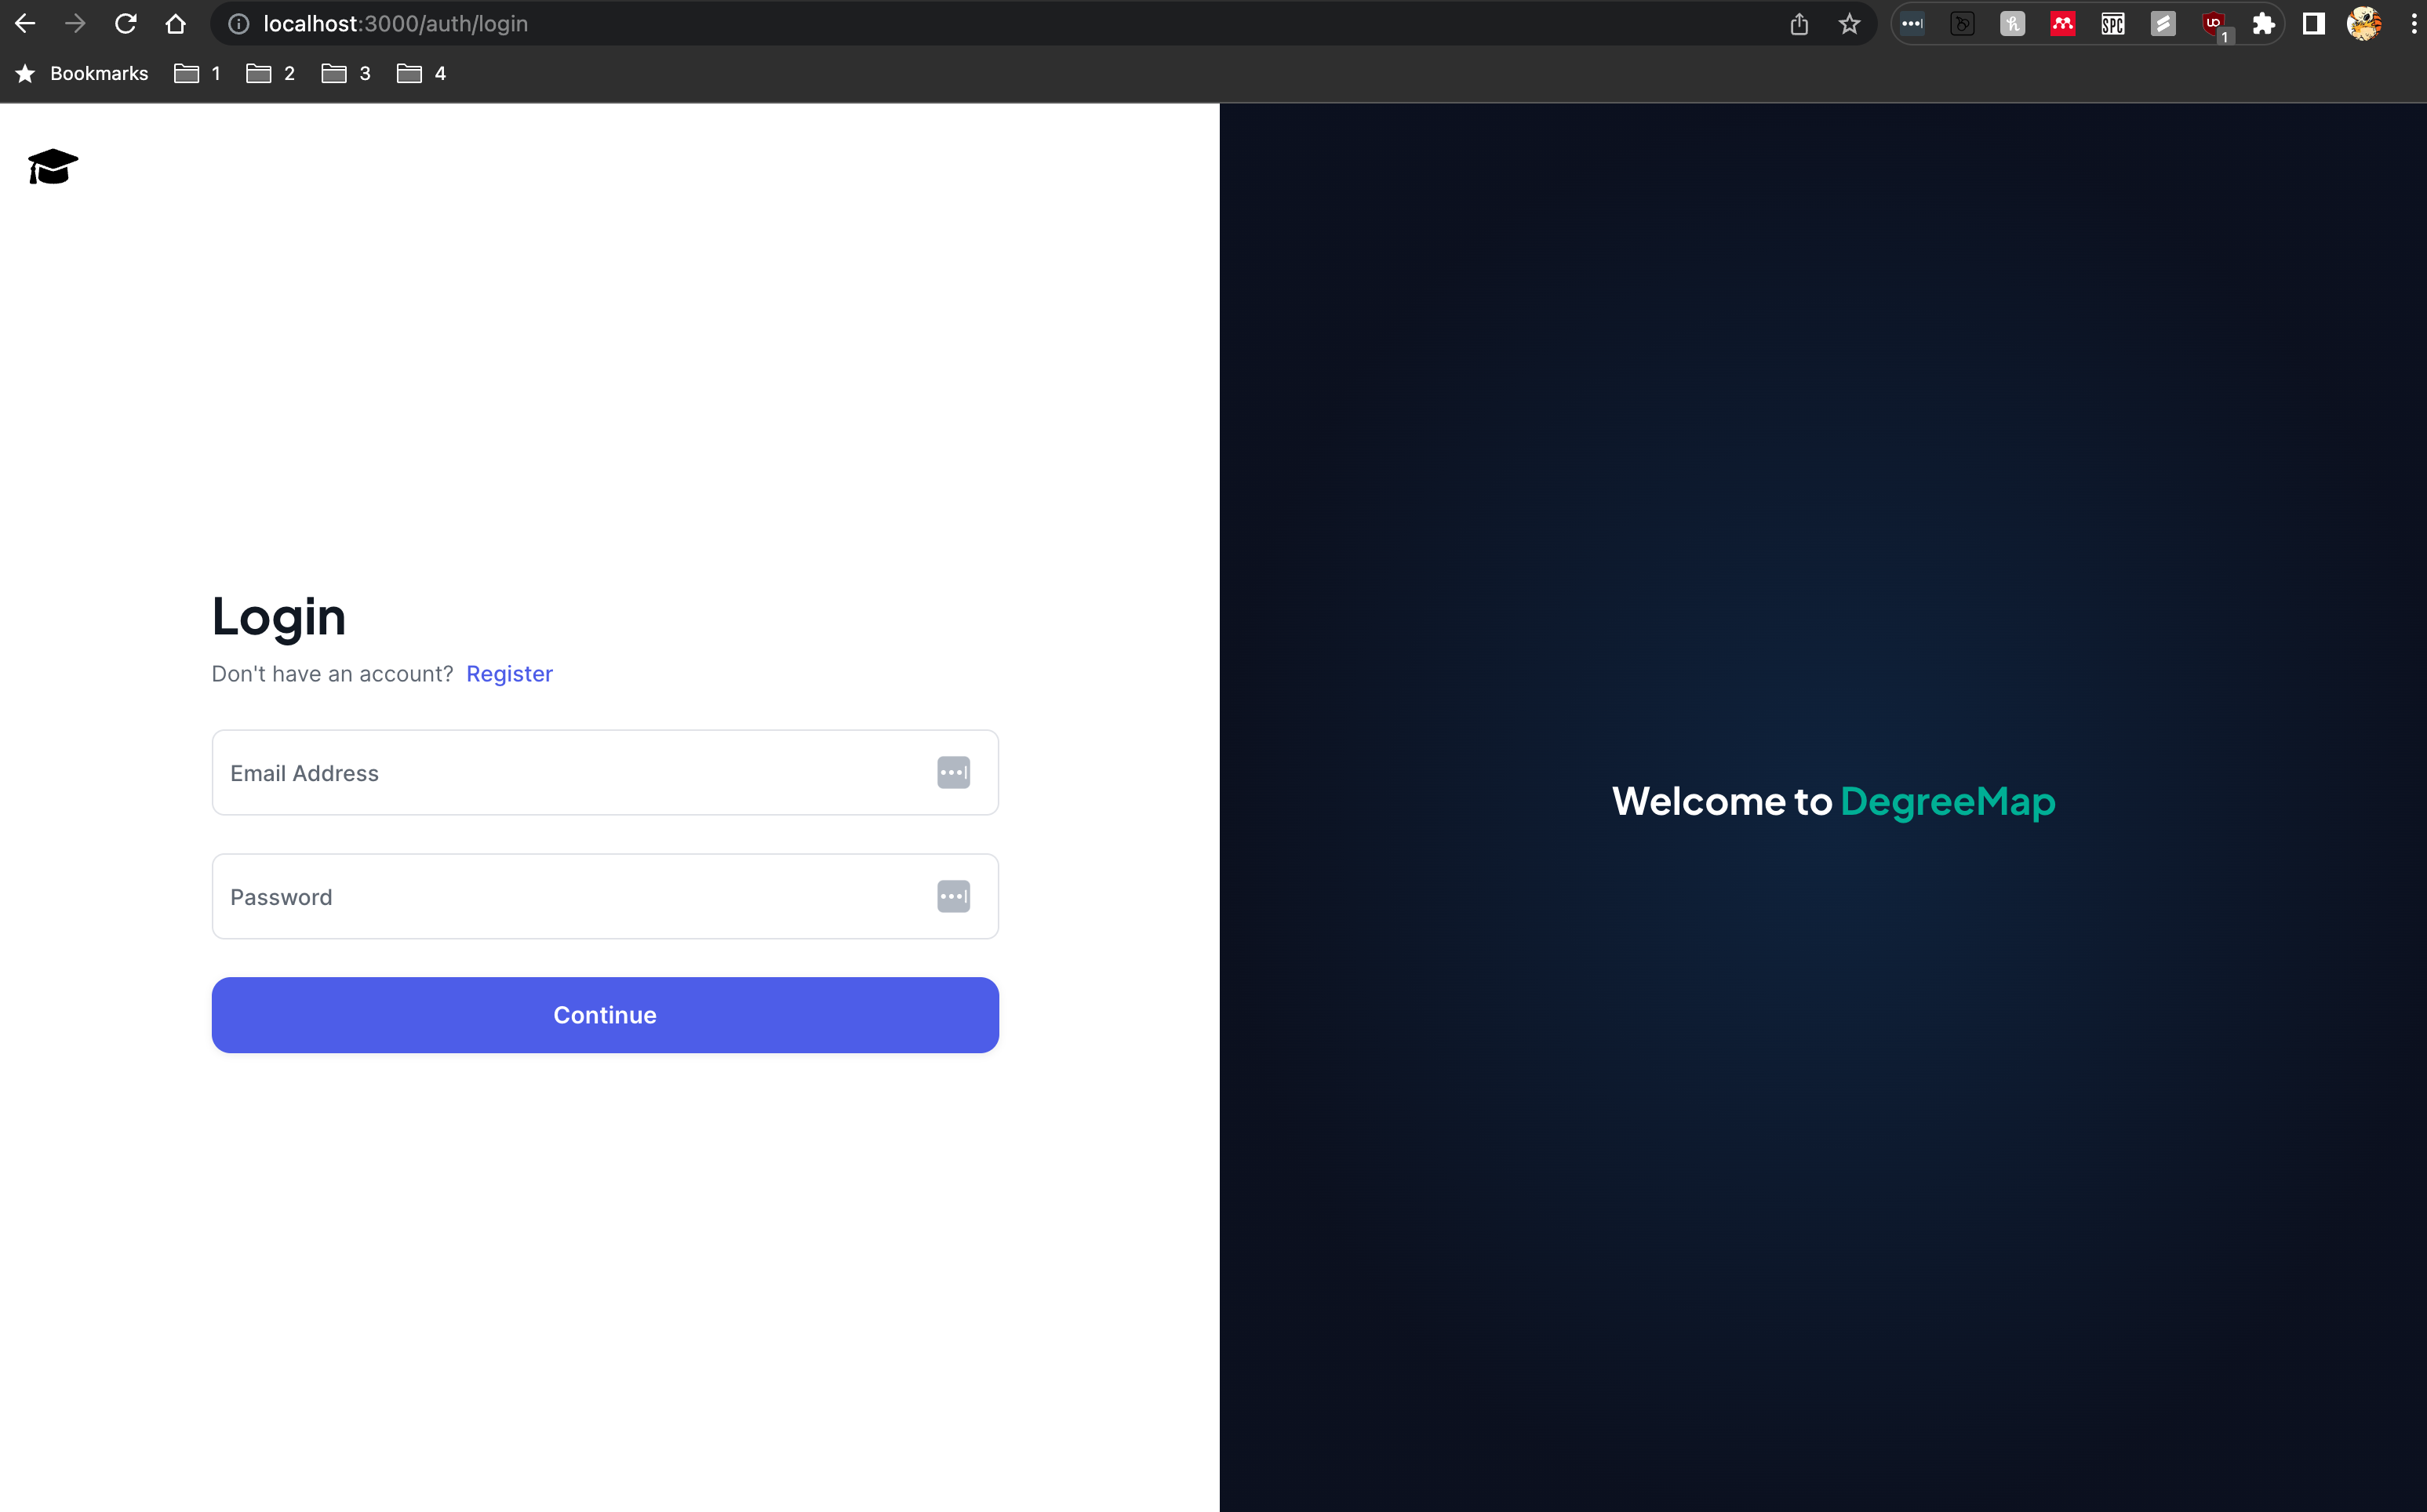
\includegraphics[width=400px]{R6/i4}
        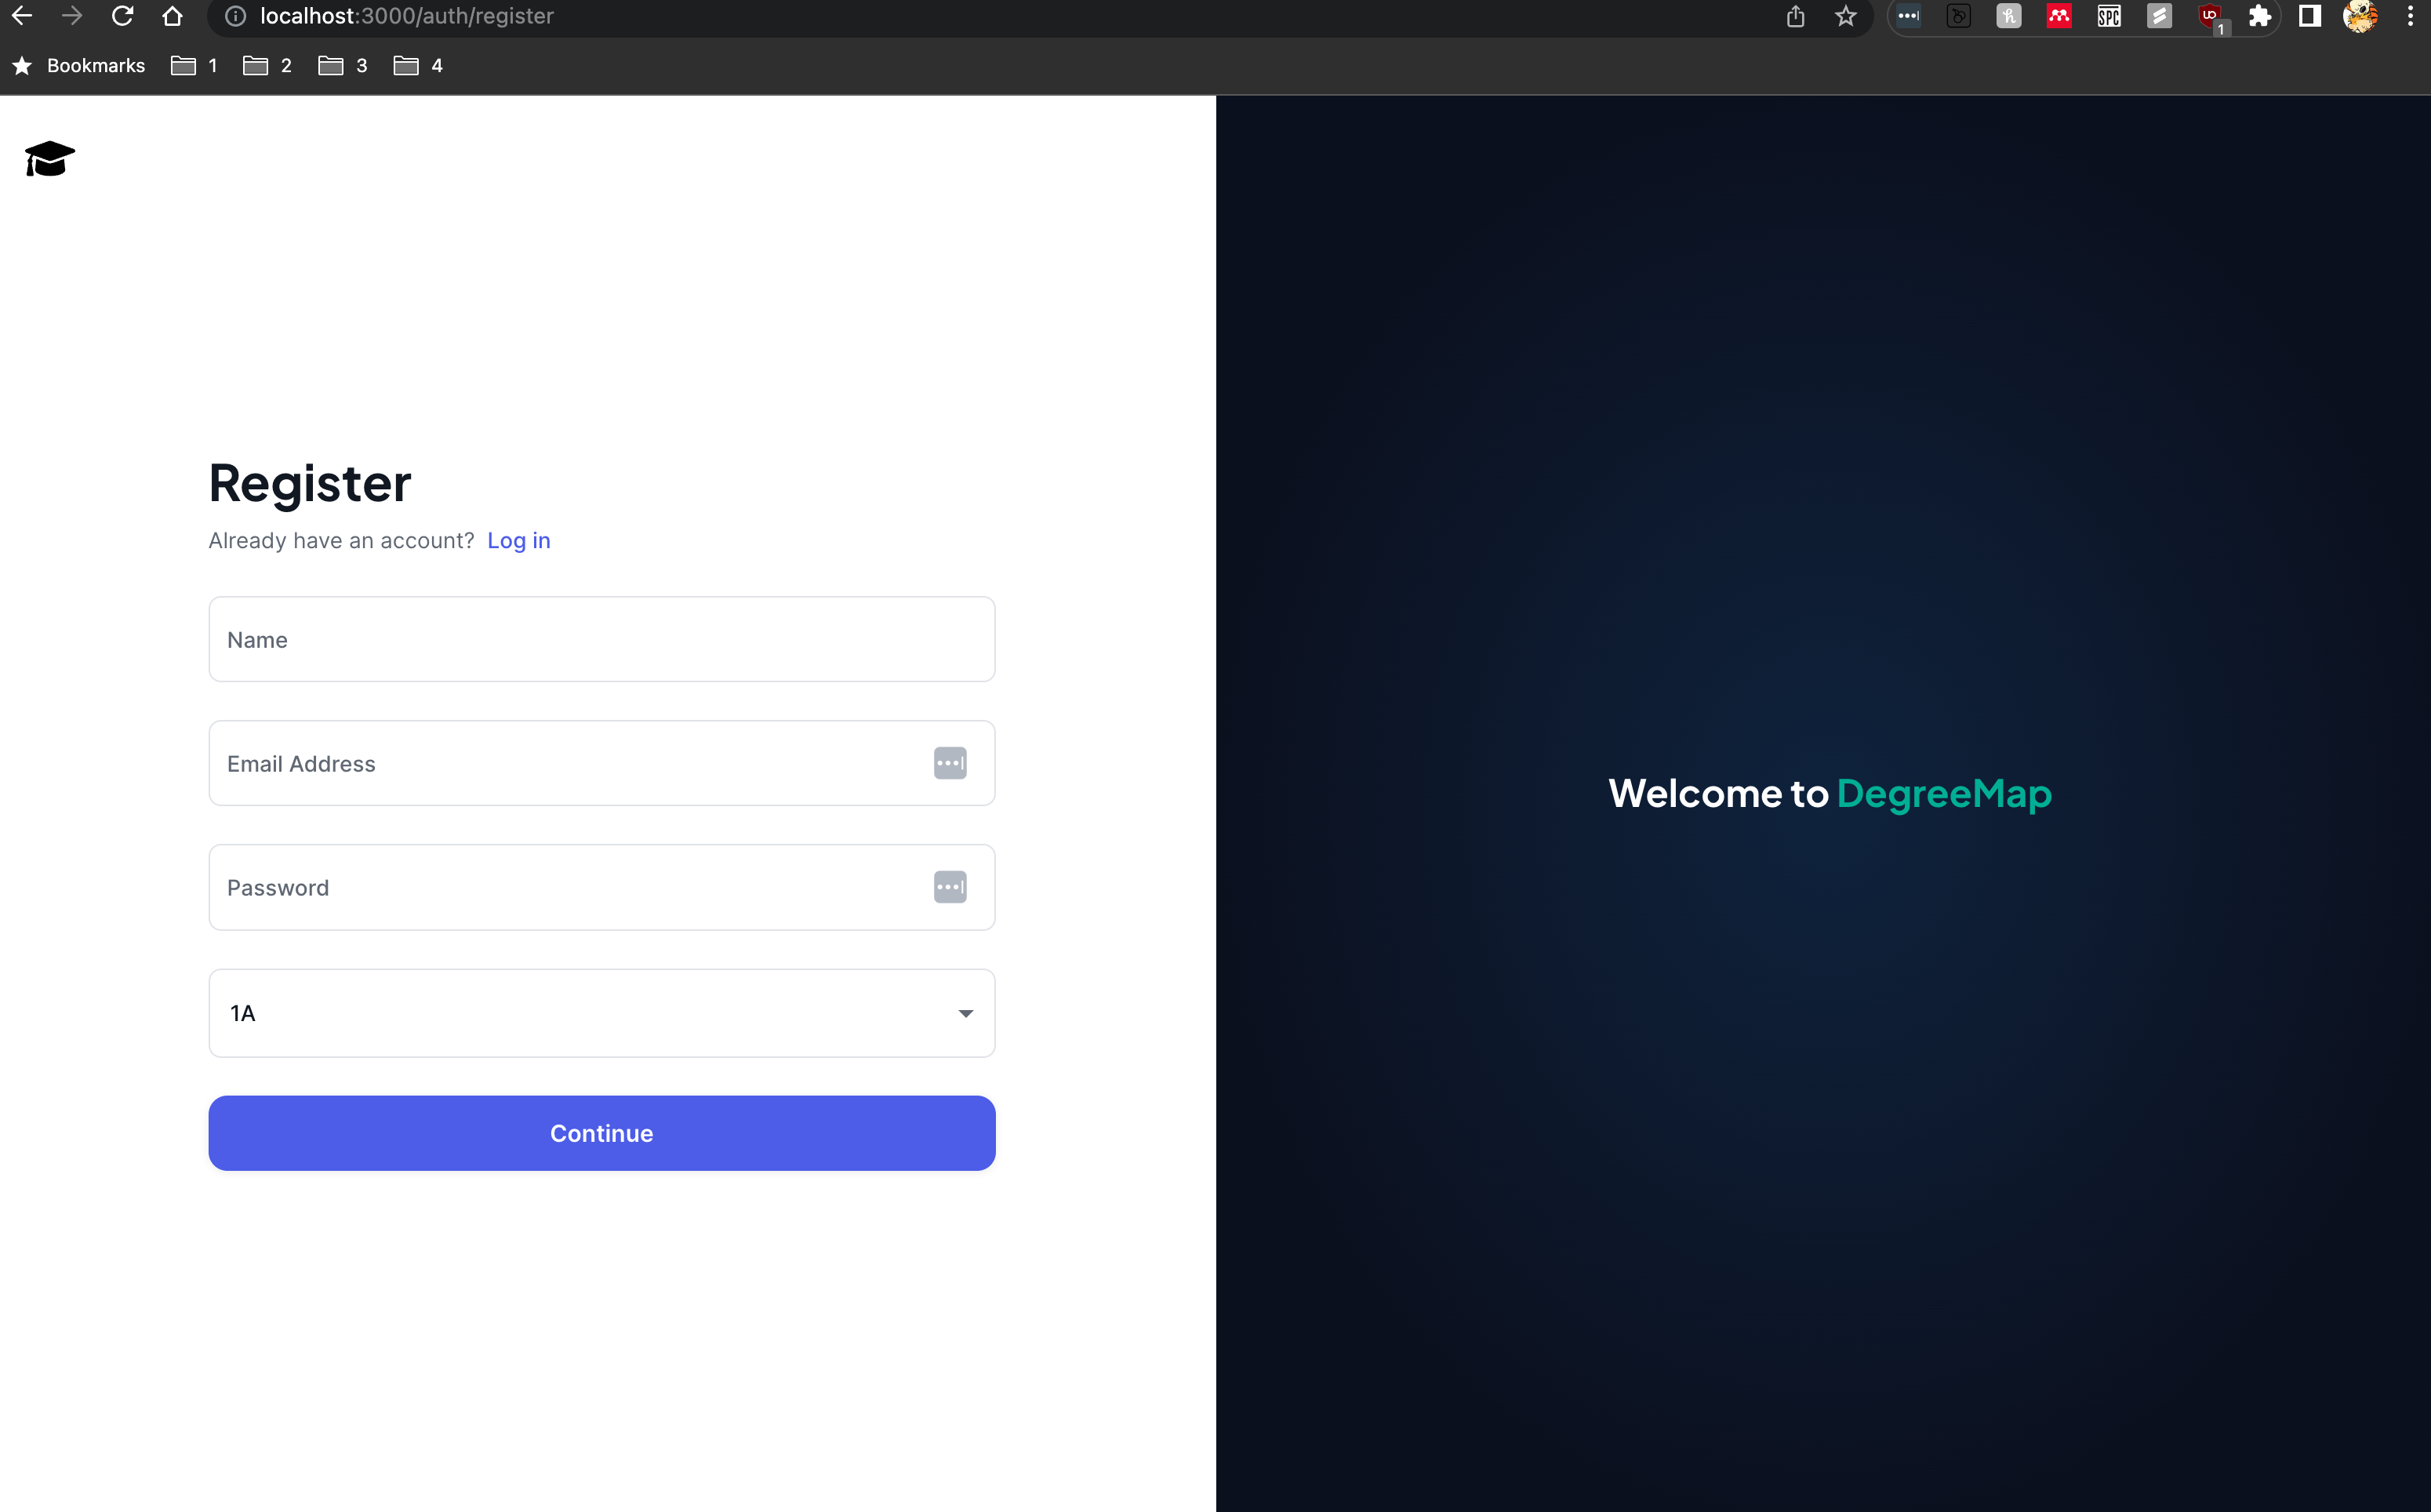
\includegraphics[width=400px]{R6/i5}
        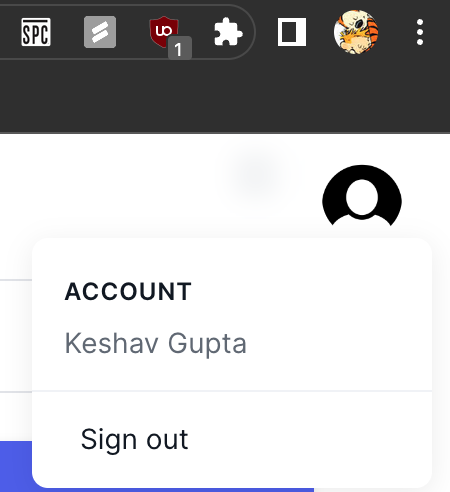
\includegraphics[width=400px]{R6/i3}
        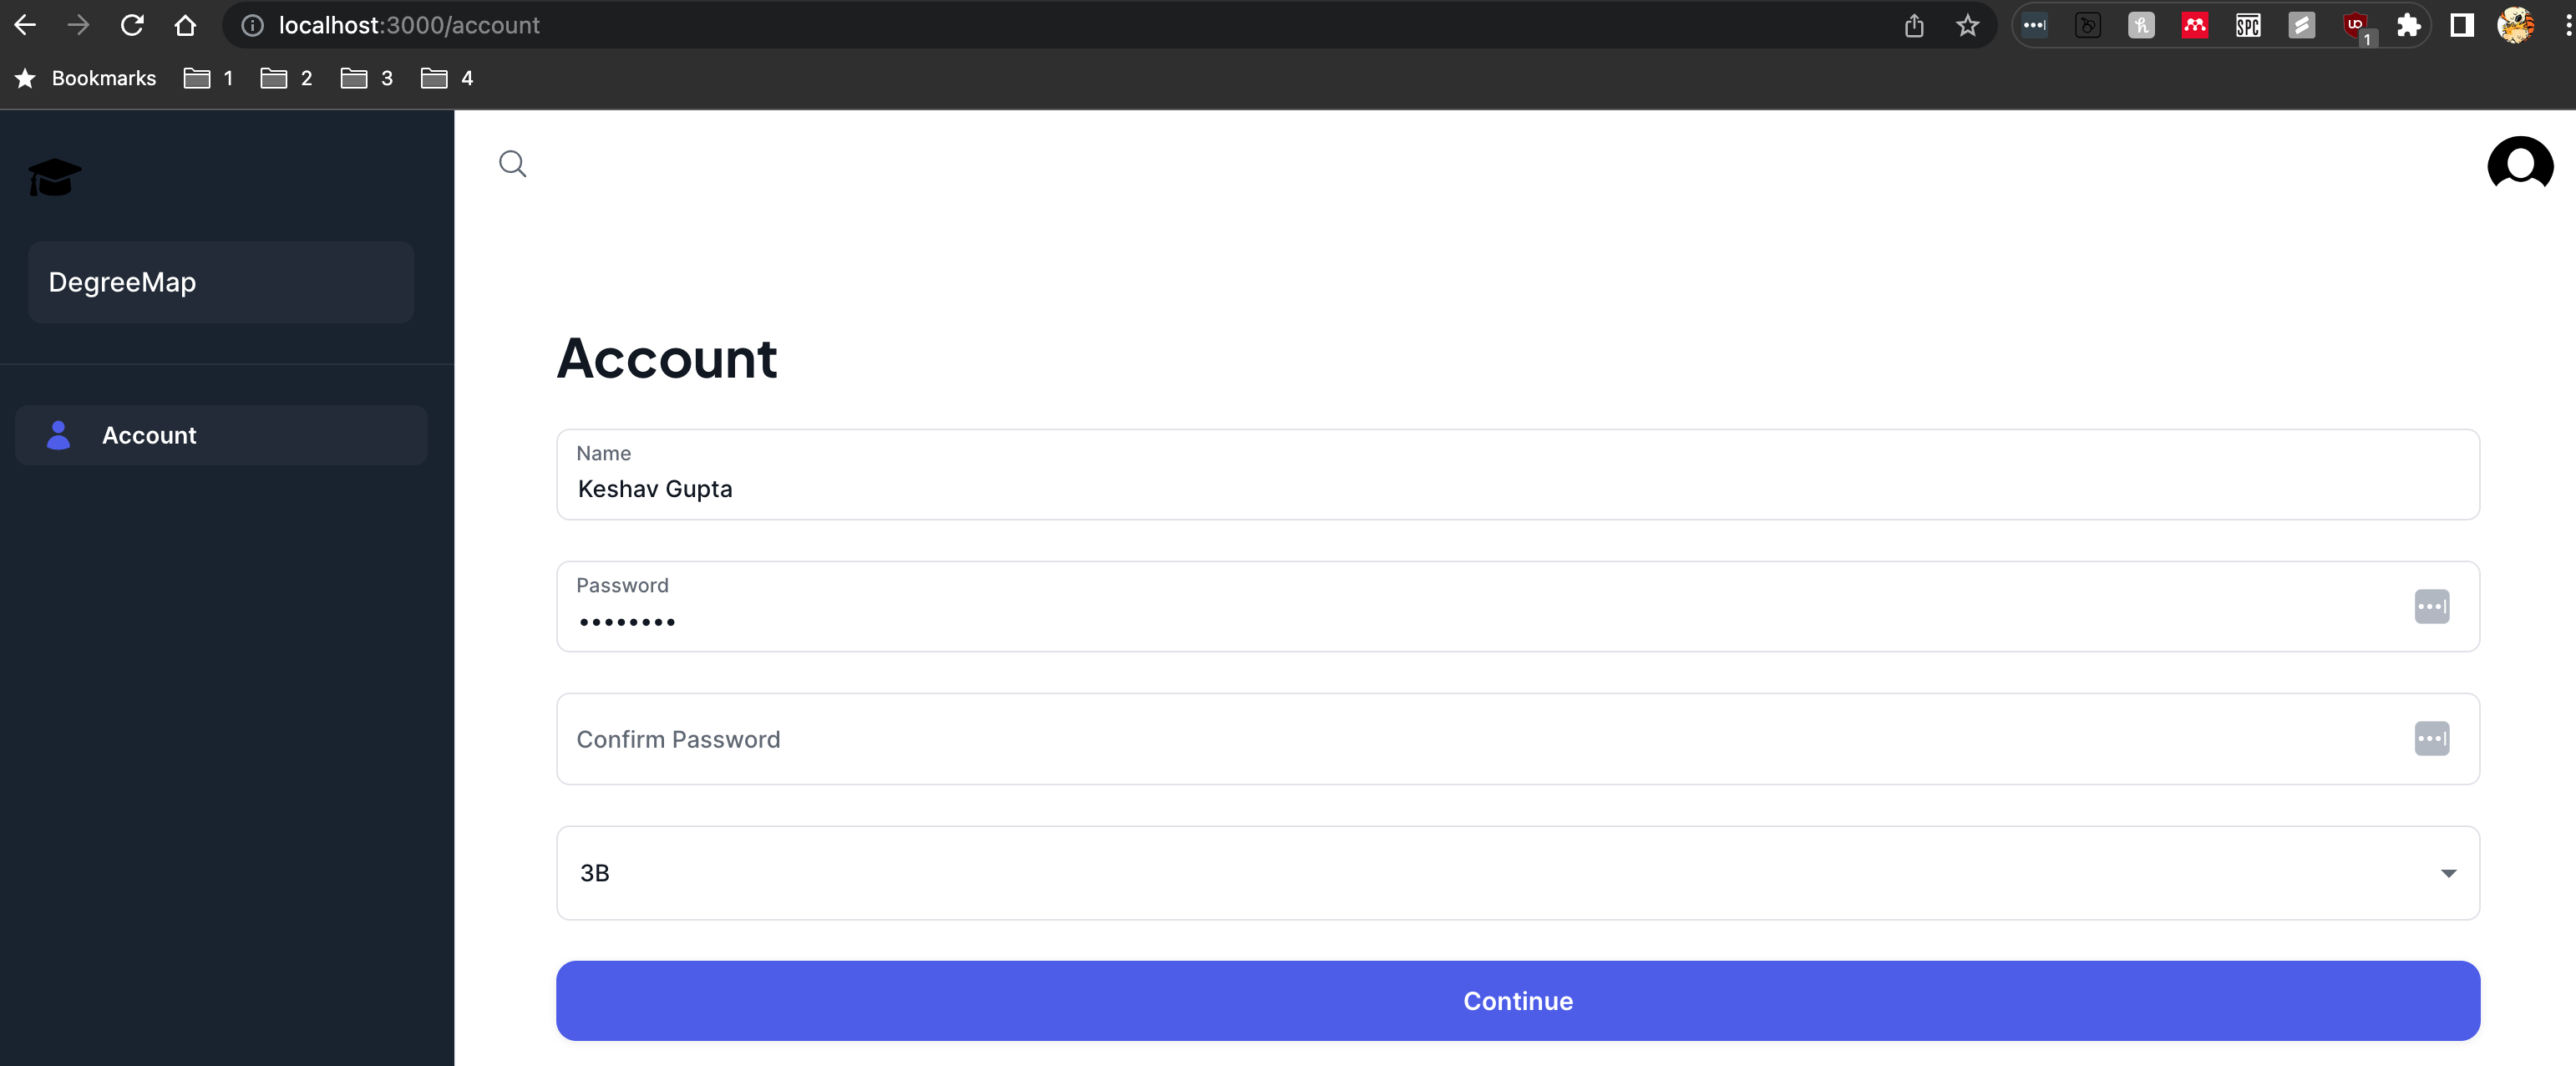
\includegraphics[width=400px]{R6/i1}
        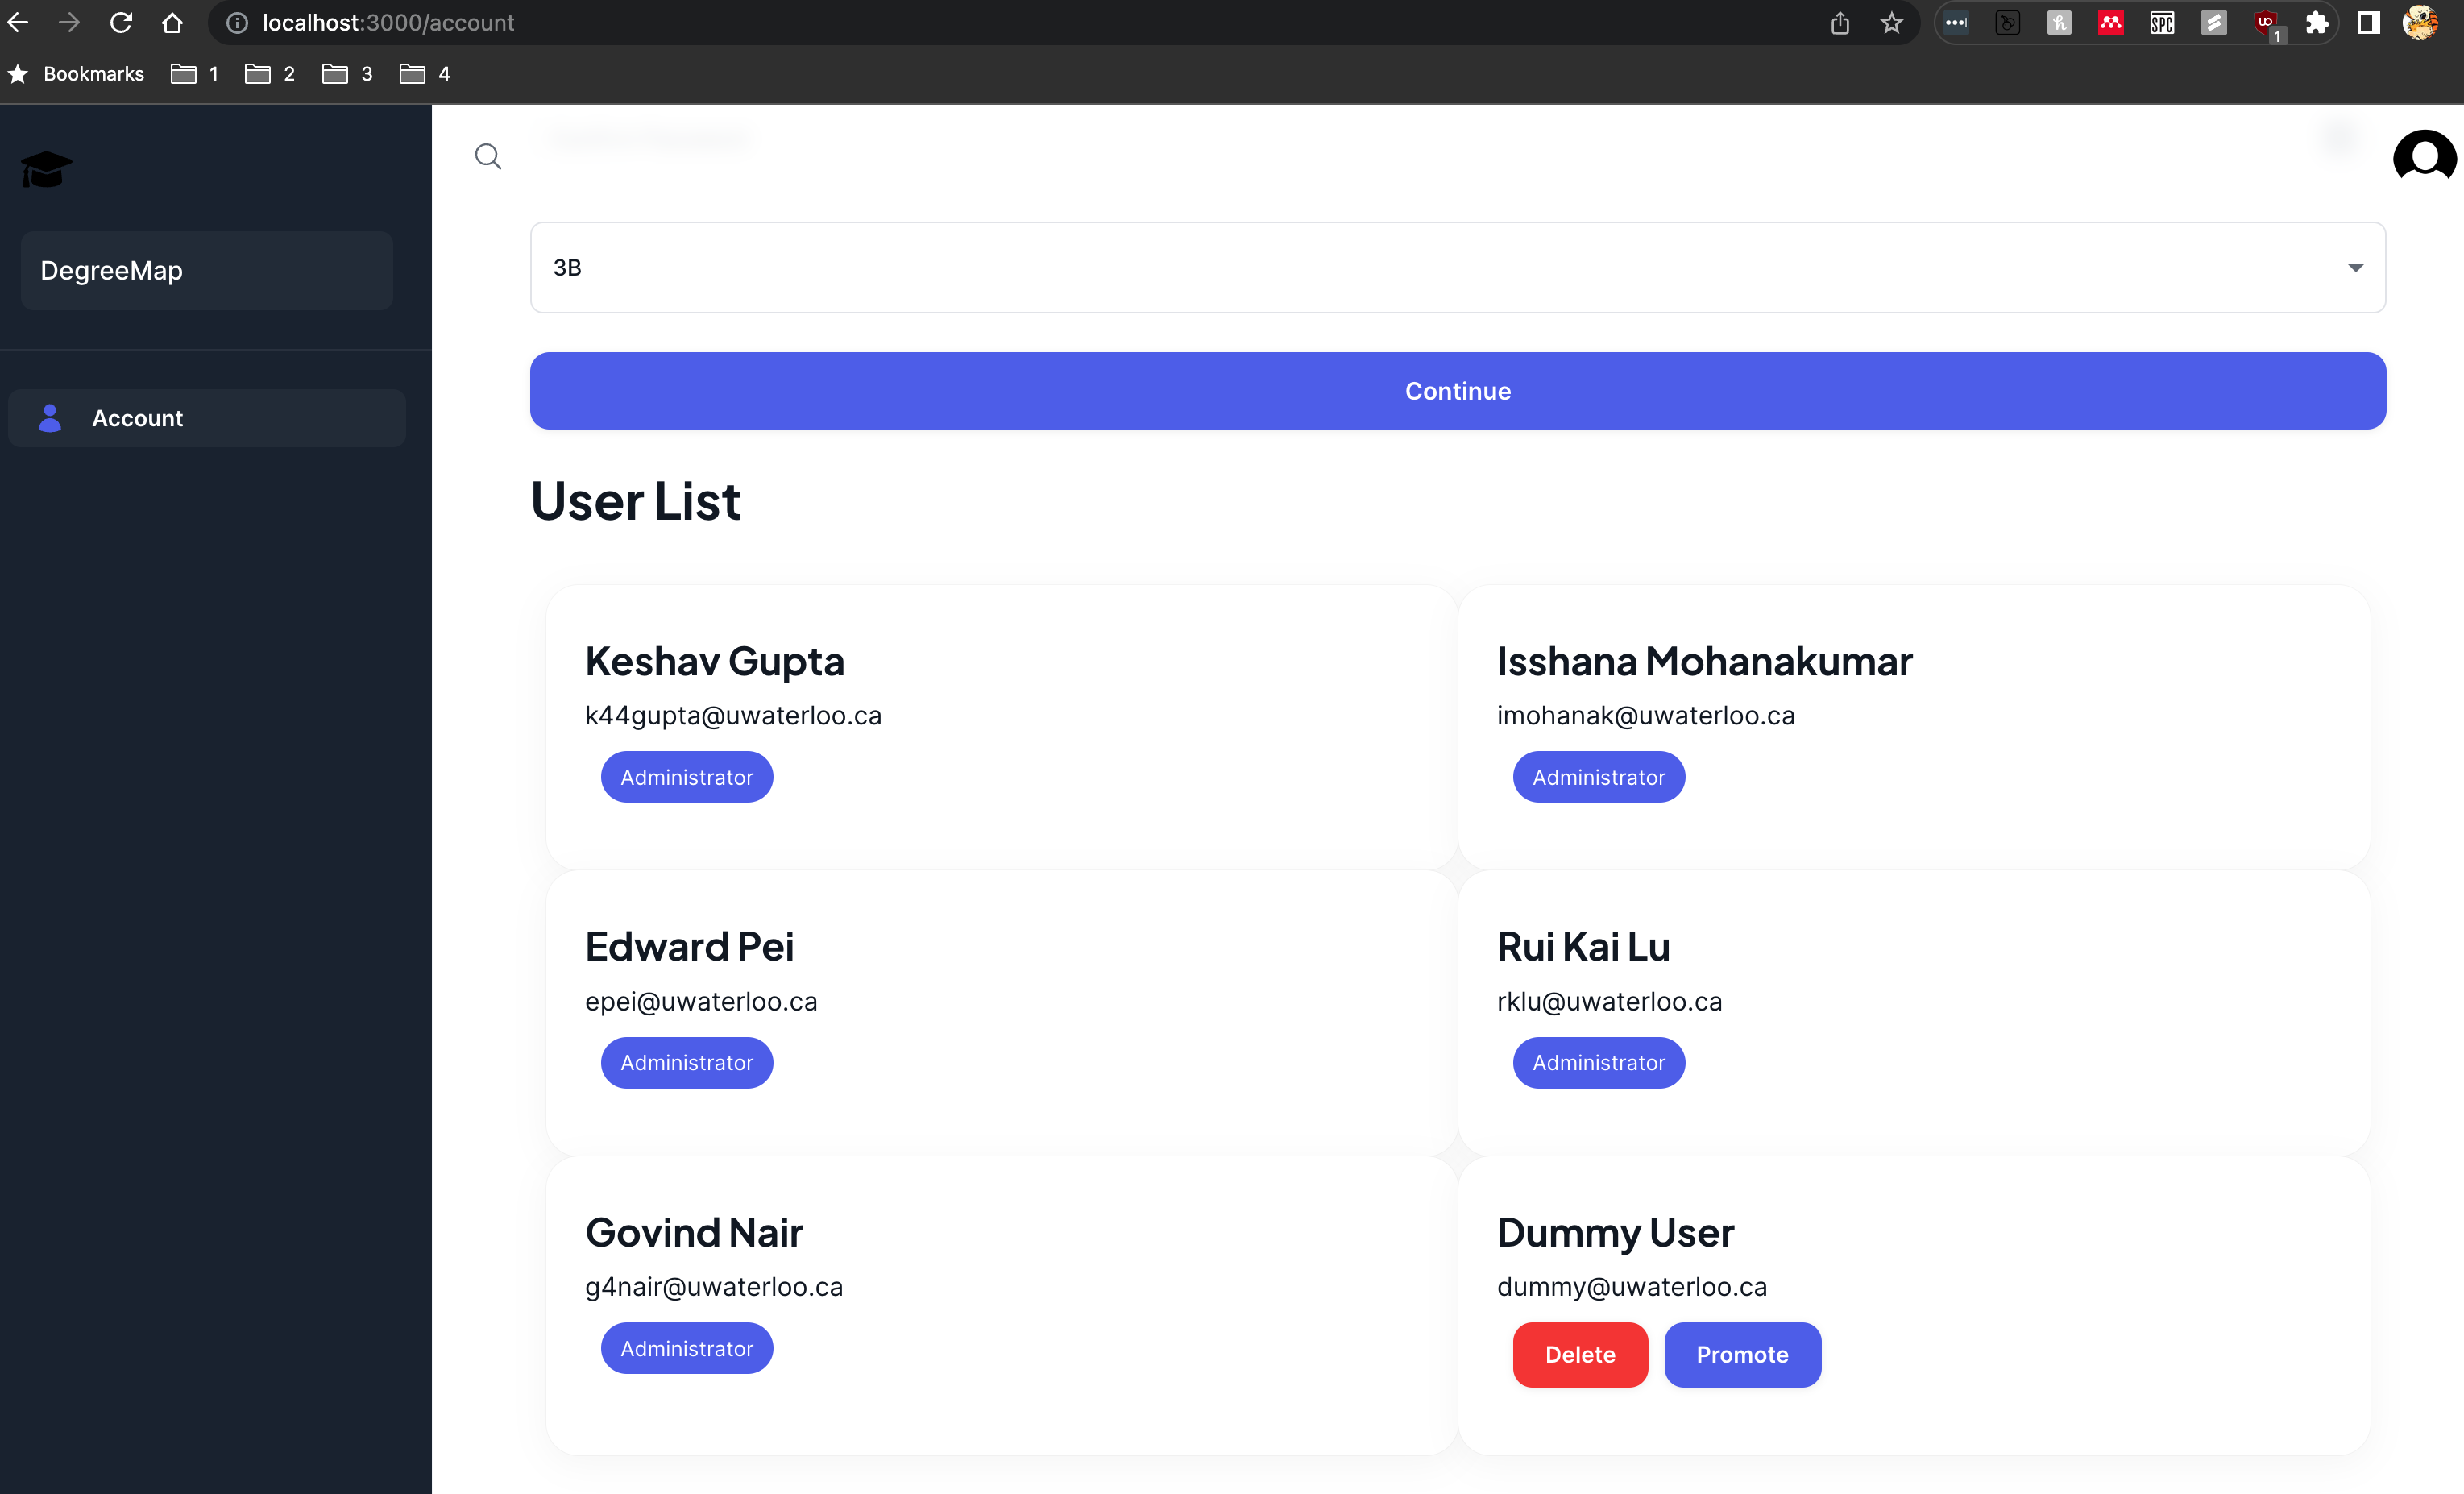
\includegraphics[width=400px]{R6/i2}
\end{center}
The testing descriptions below will assume you have started the application as described in the README.
\subsubsection*{Testing Login}
\begin{itemize}
    \item Login with incorrect email and password (type anything). Red text will appear above the blue button indicating the credentials are invalid.
    \item Try to submit with nothing entered. The empty text boxes will turn red.
    \item Login with administrator account (k44gupta@uwaterloo.ca, password). The application will be logged in, contact the database for the user object, and redirect to the main account view.
    \item Login with regular account (dummy@uwaterloo.ca, password1).  The application will be logged in, contact the database for the user object, and redirect to the main account view.
\end{itemize}
\subsubsection*{Testing Registration}
\begin{itemize}
    \item Click the 'Register' button in the login view to reach the registration page. You will be redirected to the register page.
    \item Try to submit with nothing entered. Empty text boxes will turn red.
    \item Enter anything for name, "password" for password, and leave level as "1A". Enter an already existing email in the database such as k44gupta@uwaterloo.ca, then hit the blue submit button. Red text will appear saying you already have an account.
    \item Do the same but with an email that doesn't exist already. The user will be added into the database and the app will redirect them to the home page.
    \item Do the same as above but with a password less than 8 characters long, the application will show red text saying the password is too short.
\end{itemize}
\subsubsection*{Testing Logout}
\begin{itemize}
    \item When logged in, click the top right icon that looks like a person and then press sign out. The application will redirect you to the login page.
\end{itemize}
\subsubsection*{Testing Update User}
\begin{itemize}
    \item Click the 'Account' tab on the side bar. You will be redirected to the page described in part A.
    \item Type anything for name, select any level from the dropdown, and enter anything for password. However, enter a password in confirm password that doesn't match the other password box, then hit the blue submit button. Red text will appear above the button saying the passwords don't match.
    \item Do the same but with matching passwords. Then log out and try to log in with your old details, it will no longer work. Then log in with the new password and it will log in correctly.
\end{itemize}
\subsubsection*{Testing User Management}
\begin{itemize}
    \item Log in as a regular user and go to the account tab, the user list will not show up.
    \item Log in as an admin and go to the account tab, you will see the user list.
    \item As an administrator, click delete on the dummy user. The user will disappear from the list and database.
    \item As an administrator, click the promote button. The promote and delete buttons will disappear and the administrator chip will replace them.
\end{itemize}
\section*{R7. List, Search, Add, and Delete Courses}
\label{sec:R7}
\subsection*{R7a. Interface Design}
\subsubsection*{Listing Courses}
This whole feature is important to help students more transparently search for courses that the university offers. This is the homepage of the application, a complete list of courses, each row of the list highlights the course ID, the course name, the course description, and the pre/anti-requisites. There is also a tool bar on the side of the window that allows the user to navigate to other features of the application. The list won't show any results until the user searches for a course. The main user for this feature is Waterloo students. The list will be sorted alphabetically by course subject and course number. Clicking a row will select it.
\subsubsection*{Searching Courses}
There will be a search box at the top of the list and search view. Waterloo students can select the course subject (i.e. CS, MATH, AFM, etc) and it will show all courses with that subject. The user types the subject in the text box. The user can also search by any of course title, course subject, or course number within the search bar itself. The application will show all relevant courses in the list where the search query matches any of the three criteria. The search box must have at least four characters for results to start appearing in the list and for the queries to be sent to the database. There will also be a check box in the search area with a title 'Offered This Term', which will only show courses that are offered during the term (i.e. they have available sections)
\subsubsection*{Admin Functionalities}
Specifically for administrators, when they select a row, a delete button will appear next to the search button. If the admin presses delete, the course will be deleted from the database, including all references to the course in other tables of the database.

Admins will also have access to the plus icon at the top right of the application window on the Course list page. When the icon is clicked, the application will go to the create course window. The window will contain text boxes to enter the course ID, the title of the course, a description of the course, pre-requisites, anti-requisites, etc. All text boxes must contain only alphanumeric characters and are required fields. The course code must not already be present in the course list. The given pre-requisites and anti-requisites must be courses that already exist in the database. Also, the same course can't appear in both the anti-requisite and pre-requisite list. The pre and anti-requisites are separated by commas. If the confirm button, which is next to the cancel button, is clicked, then the filled boxes are checked against the above requirements that were described. If a requirement is violated, red text above the confirm button appears saying "Invalid Course Data". If all requirements are satisfied, a success message will appear above the confirm button.

\subsection*{R7b. SQL Query, Testing With Sample Data}
The test sql file with all of these queries can be viewed here: \underline{\href{https://github.com/Kggupta/DegreeMap/tree/main/Database/Queries/TestSample}{TestSample/R7.sql}}, \underline{\href{https://github.com/Kggupta/DegreeMap/tree/main/Database/Queries/TestSample}{TestSample/R7.out}}. All SQL queries are commented to explain what it does for this feature.
\begin{center}
    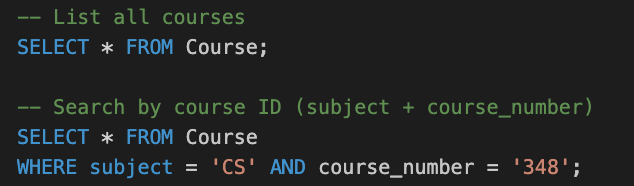
\includegraphics[width=400px]{R7/q1}
    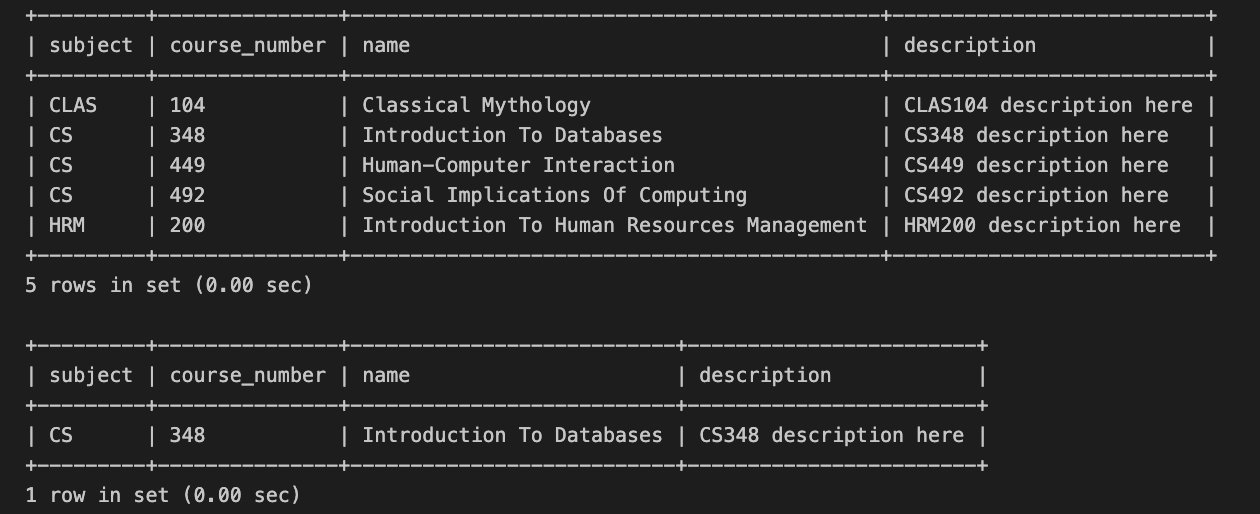
\includegraphics[width=400px]{R7/q1out}
\end{center}
The above query shows how a full list of all the courses and their information would be retrieved. It also shows a query that does an exact match to search for a course (CS 348 in this case). This is the most basic query related to this feature.

\begin{center}
    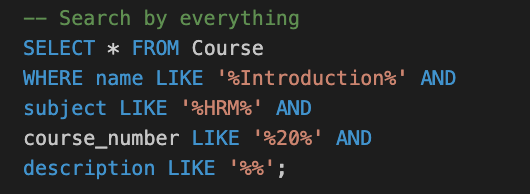
\includegraphics[width=400px]{R7/q2}
    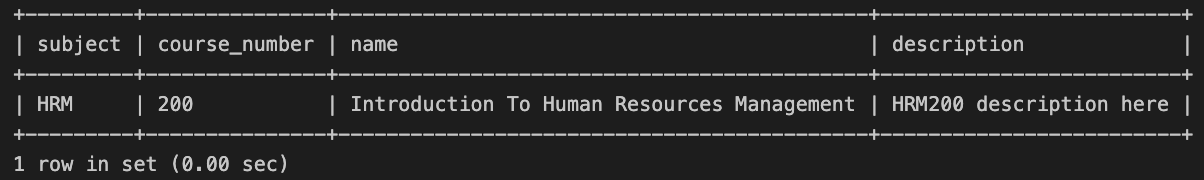
\includegraphics[width=400px]{R7/q2out}
\end{center}
The above query shows the query structure for how a search would occur. The user would be able to search by any of the fields of Course, and the server would dynamically adjust the query (such as removing the AND description... condition) based on the boxes the user indicates that they want to search by.
\begin{center}
    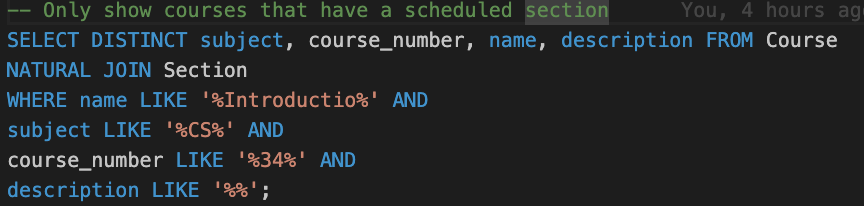
\includegraphics[width=400px]{R7/q3}
    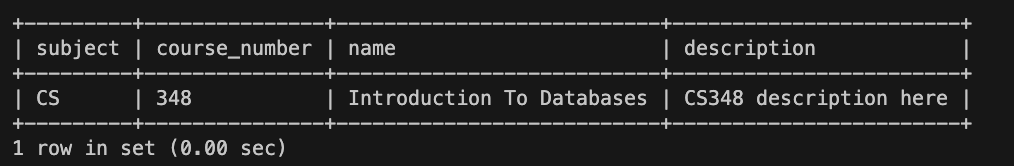
\includegraphics[width=400px]{R7/q3out}
\end{center}
The above query specifically only returns the courses that have at least one offered section. This would be a filter the user can select in the user interface.
\begin{center}
    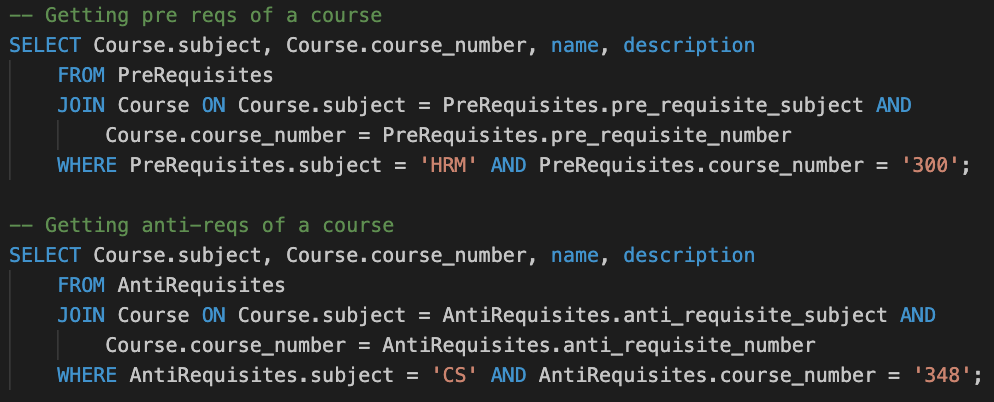
\includegraphics[width=400px]{R7/q4}
    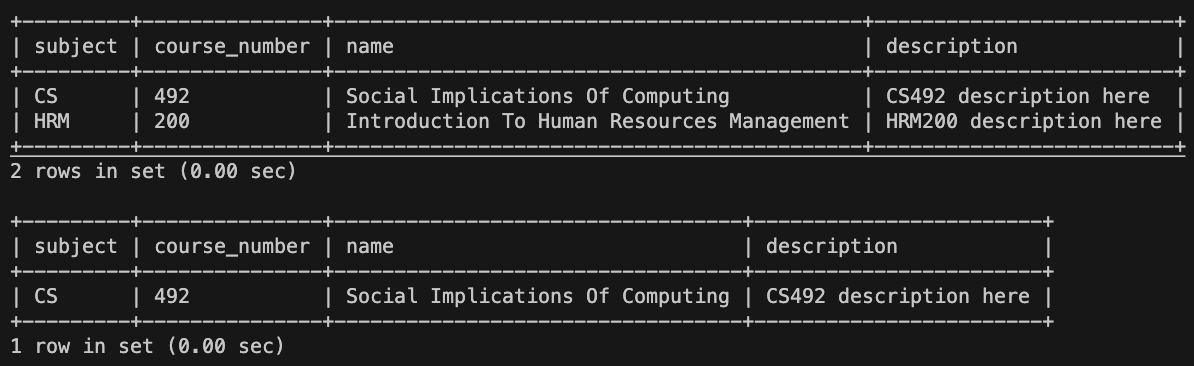
\includegraphics[width=400px]{R7/q4out}
\end{center}
The above query gets the pre/anti-requisite course information about a specific course. In this case, HRM 200 has pre-requisites CS492 and HRM200 (yes that is not possible in reality, but this is just the sample data set). CS348 has the anti-requisite CS492.
\subsection*{R7c. SQL Query, Testing With Production Data}
The test sql file with all of these queries can be viewed here: \underline{\href{https://github.com/Kggupta/DegreeMap/tree/main/Database/Queries/TestProduction}{TestProduction/R7.sql}}, \underline{\href{https://github.com/Kggupta/DegreeMap/tree/main/Database/Queries/TestProduction}{TestProduction/R7.out}}. All SQL queries are commented to explain what it does for this feature.

We created  procedures in \textbf{Queries/Procedures.sql} for the searching feature.

We also realized that wildcards are very inefficient when used in the form of '\%text\%', instead it's better to only use the wildcard at the start or at the end of the string. Also, since we are using the '\%text\%' format on the course subject and course number columns, there is room for improvement. Knowing that MySQL automatically puts indexes on primary keys (which is course subject and course number in this case), we can replace the wildcards with just this format: 'text\%'. While this does change the logic of the query, speaking practically, most users tend to search for course at the start of the string and not in the middle. For example, users are obviously more likely to search for 'PMATH' by typing 'PM...' first, they wouldn't start by typing 'ATH'. We didn't apply the same change to course title and course description, because sometimes people only remember part of a title or description such as 'Database' inside 'Introduction to Databases'. With that in mind, we updated the SQL Queries with the new wildcard format shown below. 
\begin{center}
    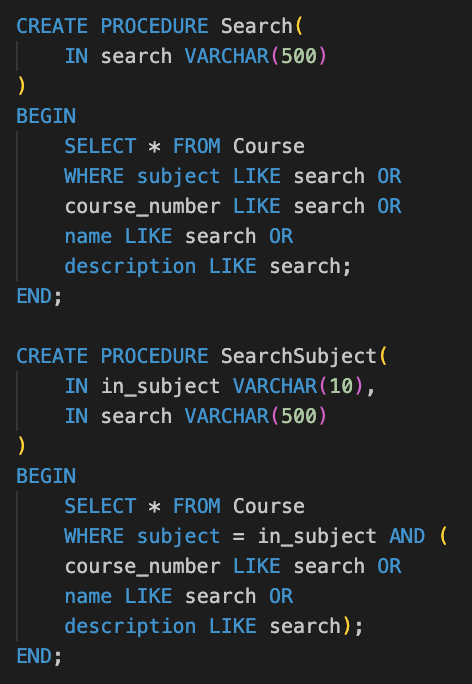
\includegraphics[width=200px]{images/R7/pq1}
    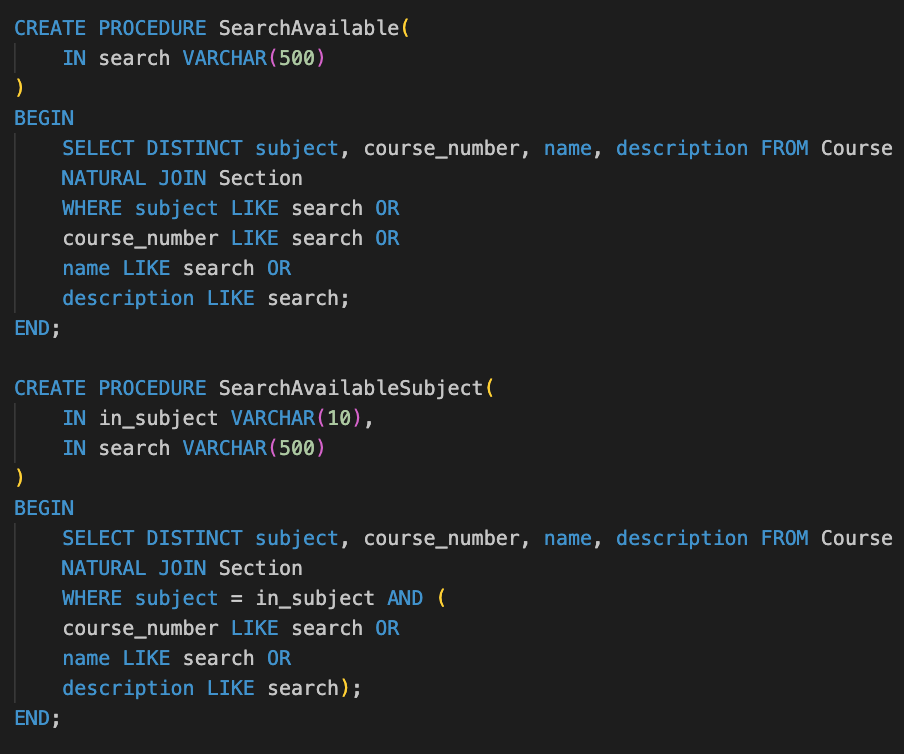
\includegraphics[width=200px]{images/R7/pq2}
    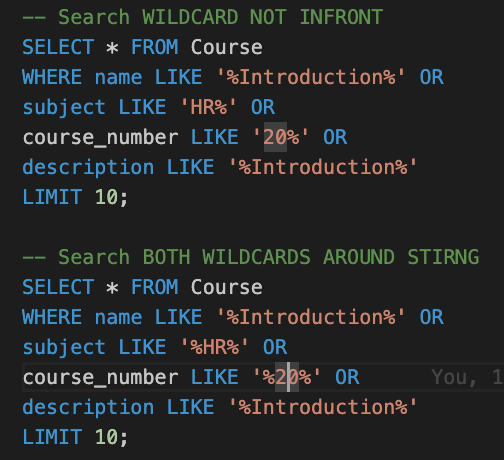
\includegraphics[width=400px]{images/R7/wildcard}
\end{center}

Note that the production sql file doesn't use the procedure since the output is thousands of rows and we want to use LIMIT to keep the output file a reasonable length. But the query themselves are the same as the procedure body so the functionality is the same.

We tested the performance difference by running the two different query formats 10 times each. We found that the version with wildcards on both sides had an average execution time of 1.1sec, while the one with only the wildcard at the end of the string had an average execution time of 0.6sec. An instance of this test is available in the test production files that is attached at the start of this section.
\subsection*{R7d. Implementation, Snapshot, Testing}
Below are screenshots of the application showing listing courses, searching for courses, deleting courses, and adding courses in that order.
The code files are highlighted in the \textbf{Current Features} section of the README in the repository.
\begin{center}
    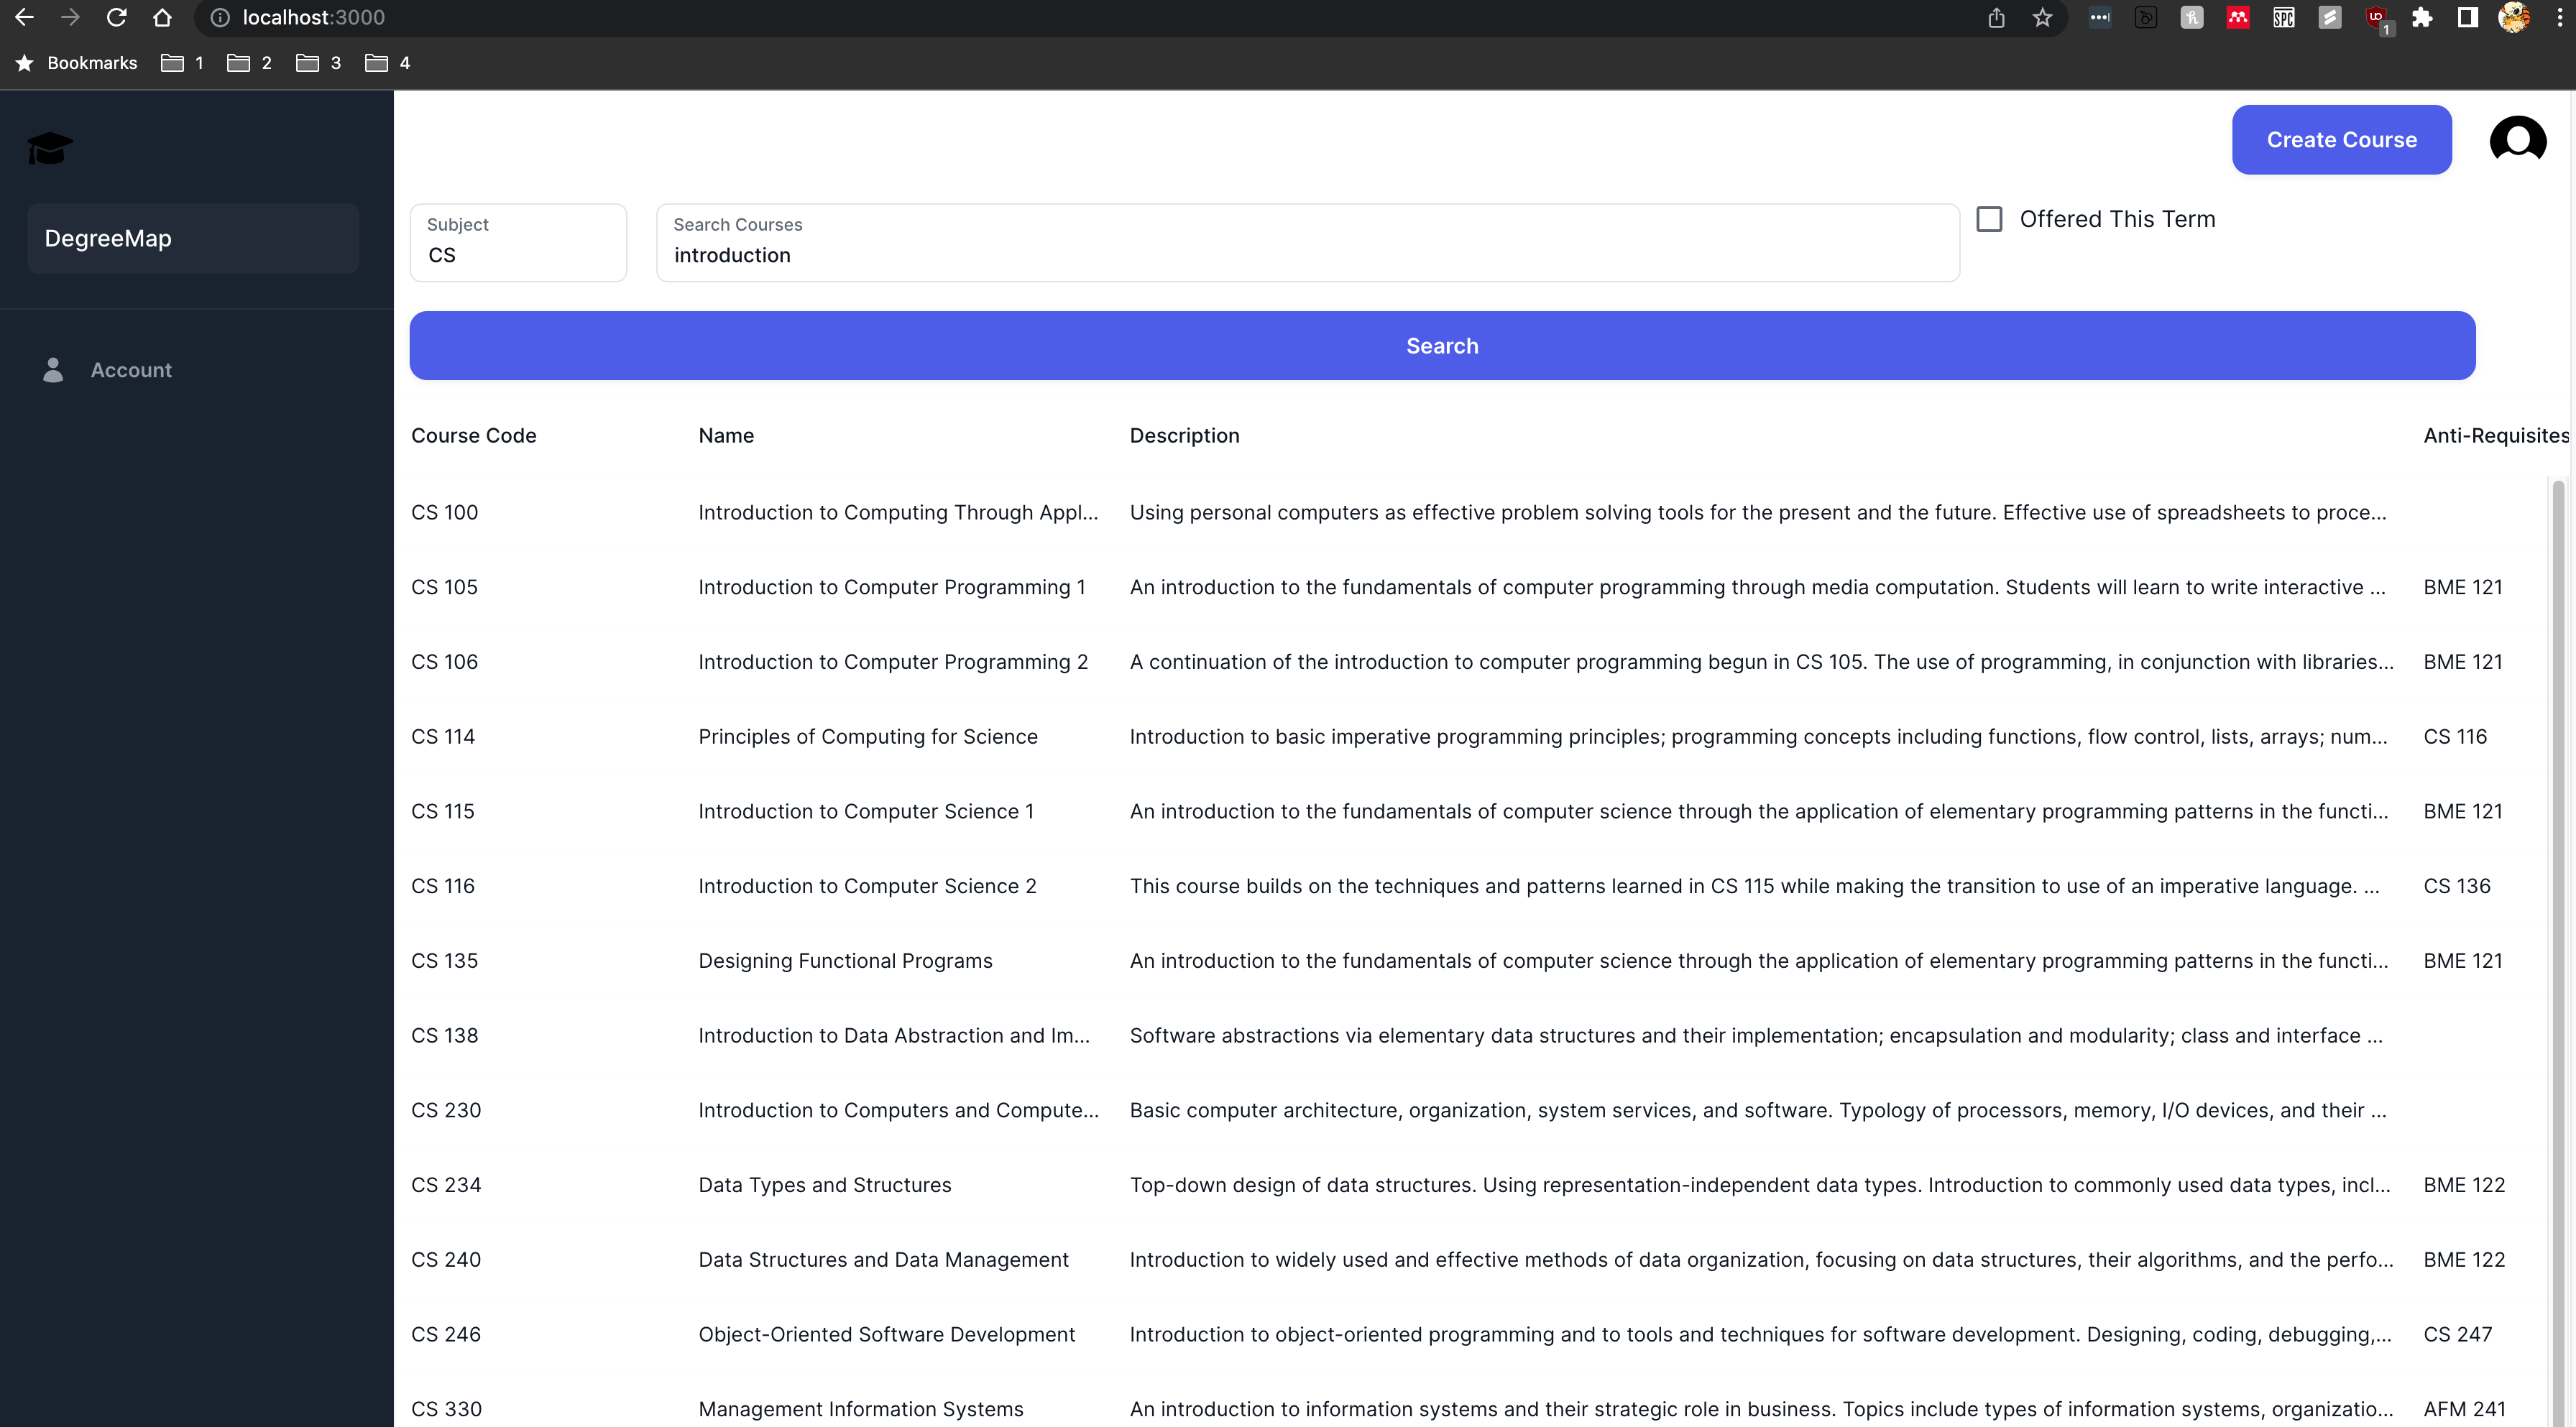
\includegraphics[width=400px]{images/R7/i1}
    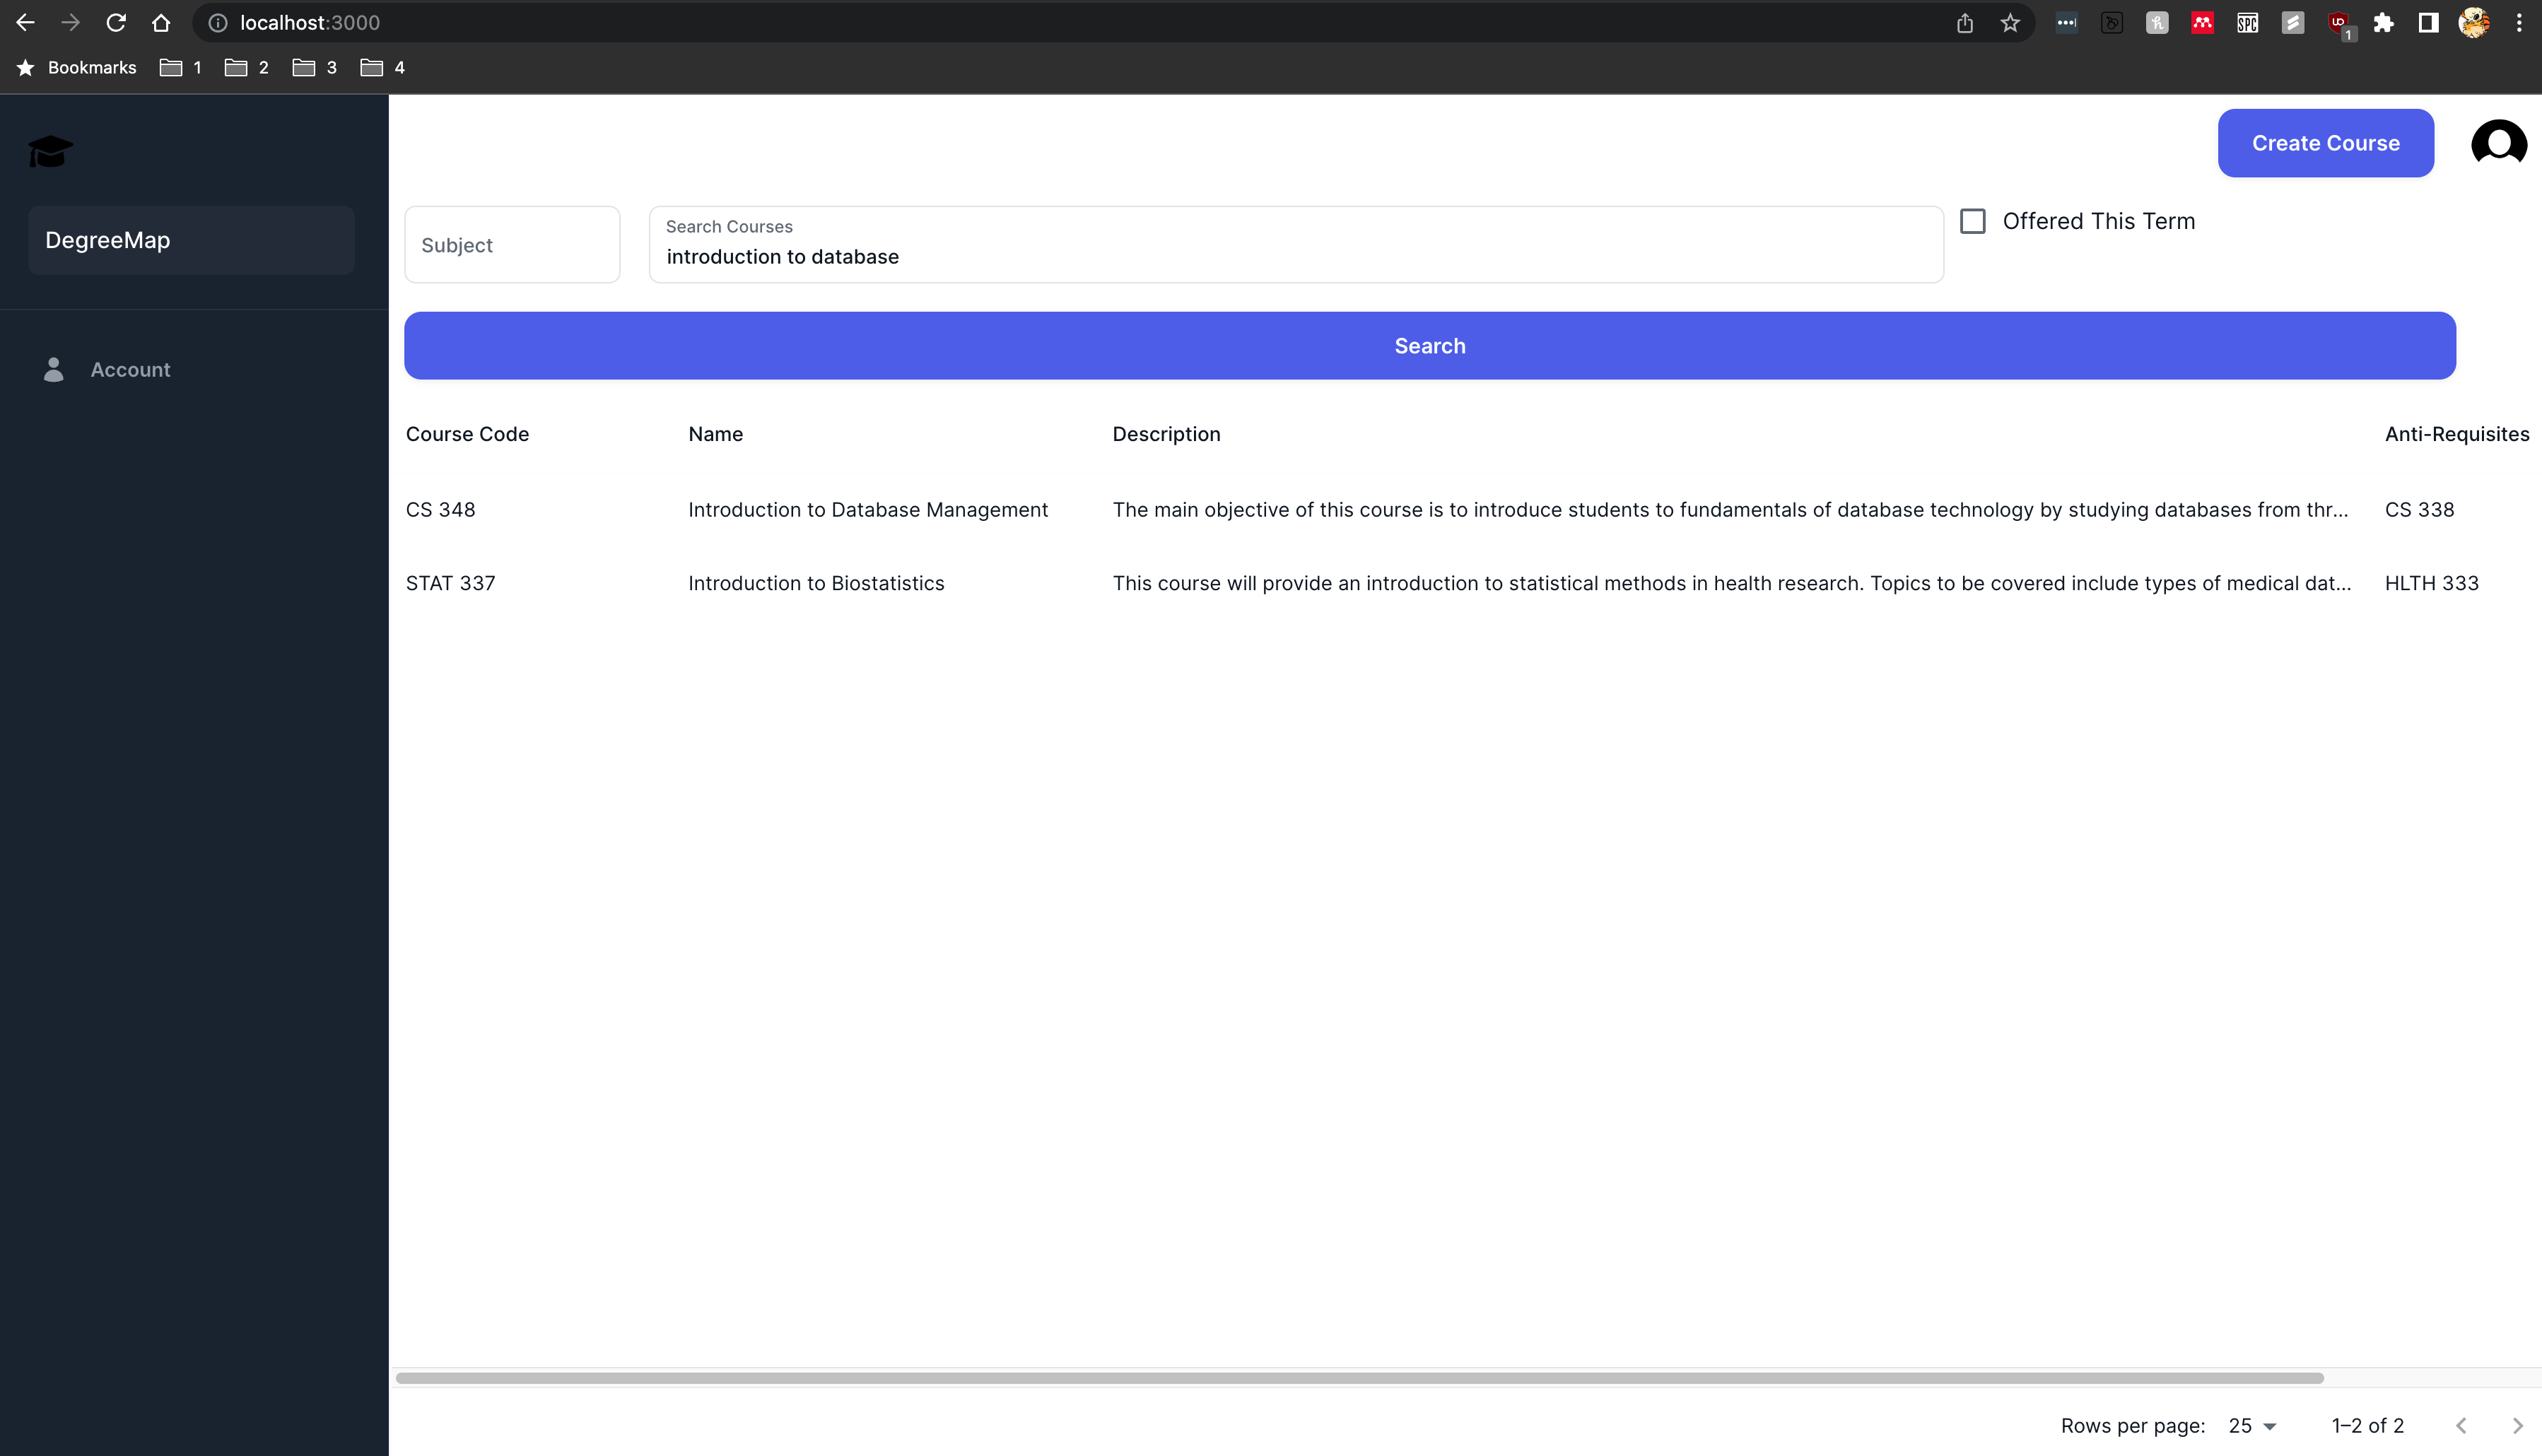
\includegraphics[width=400px]{images/R7/i2}
    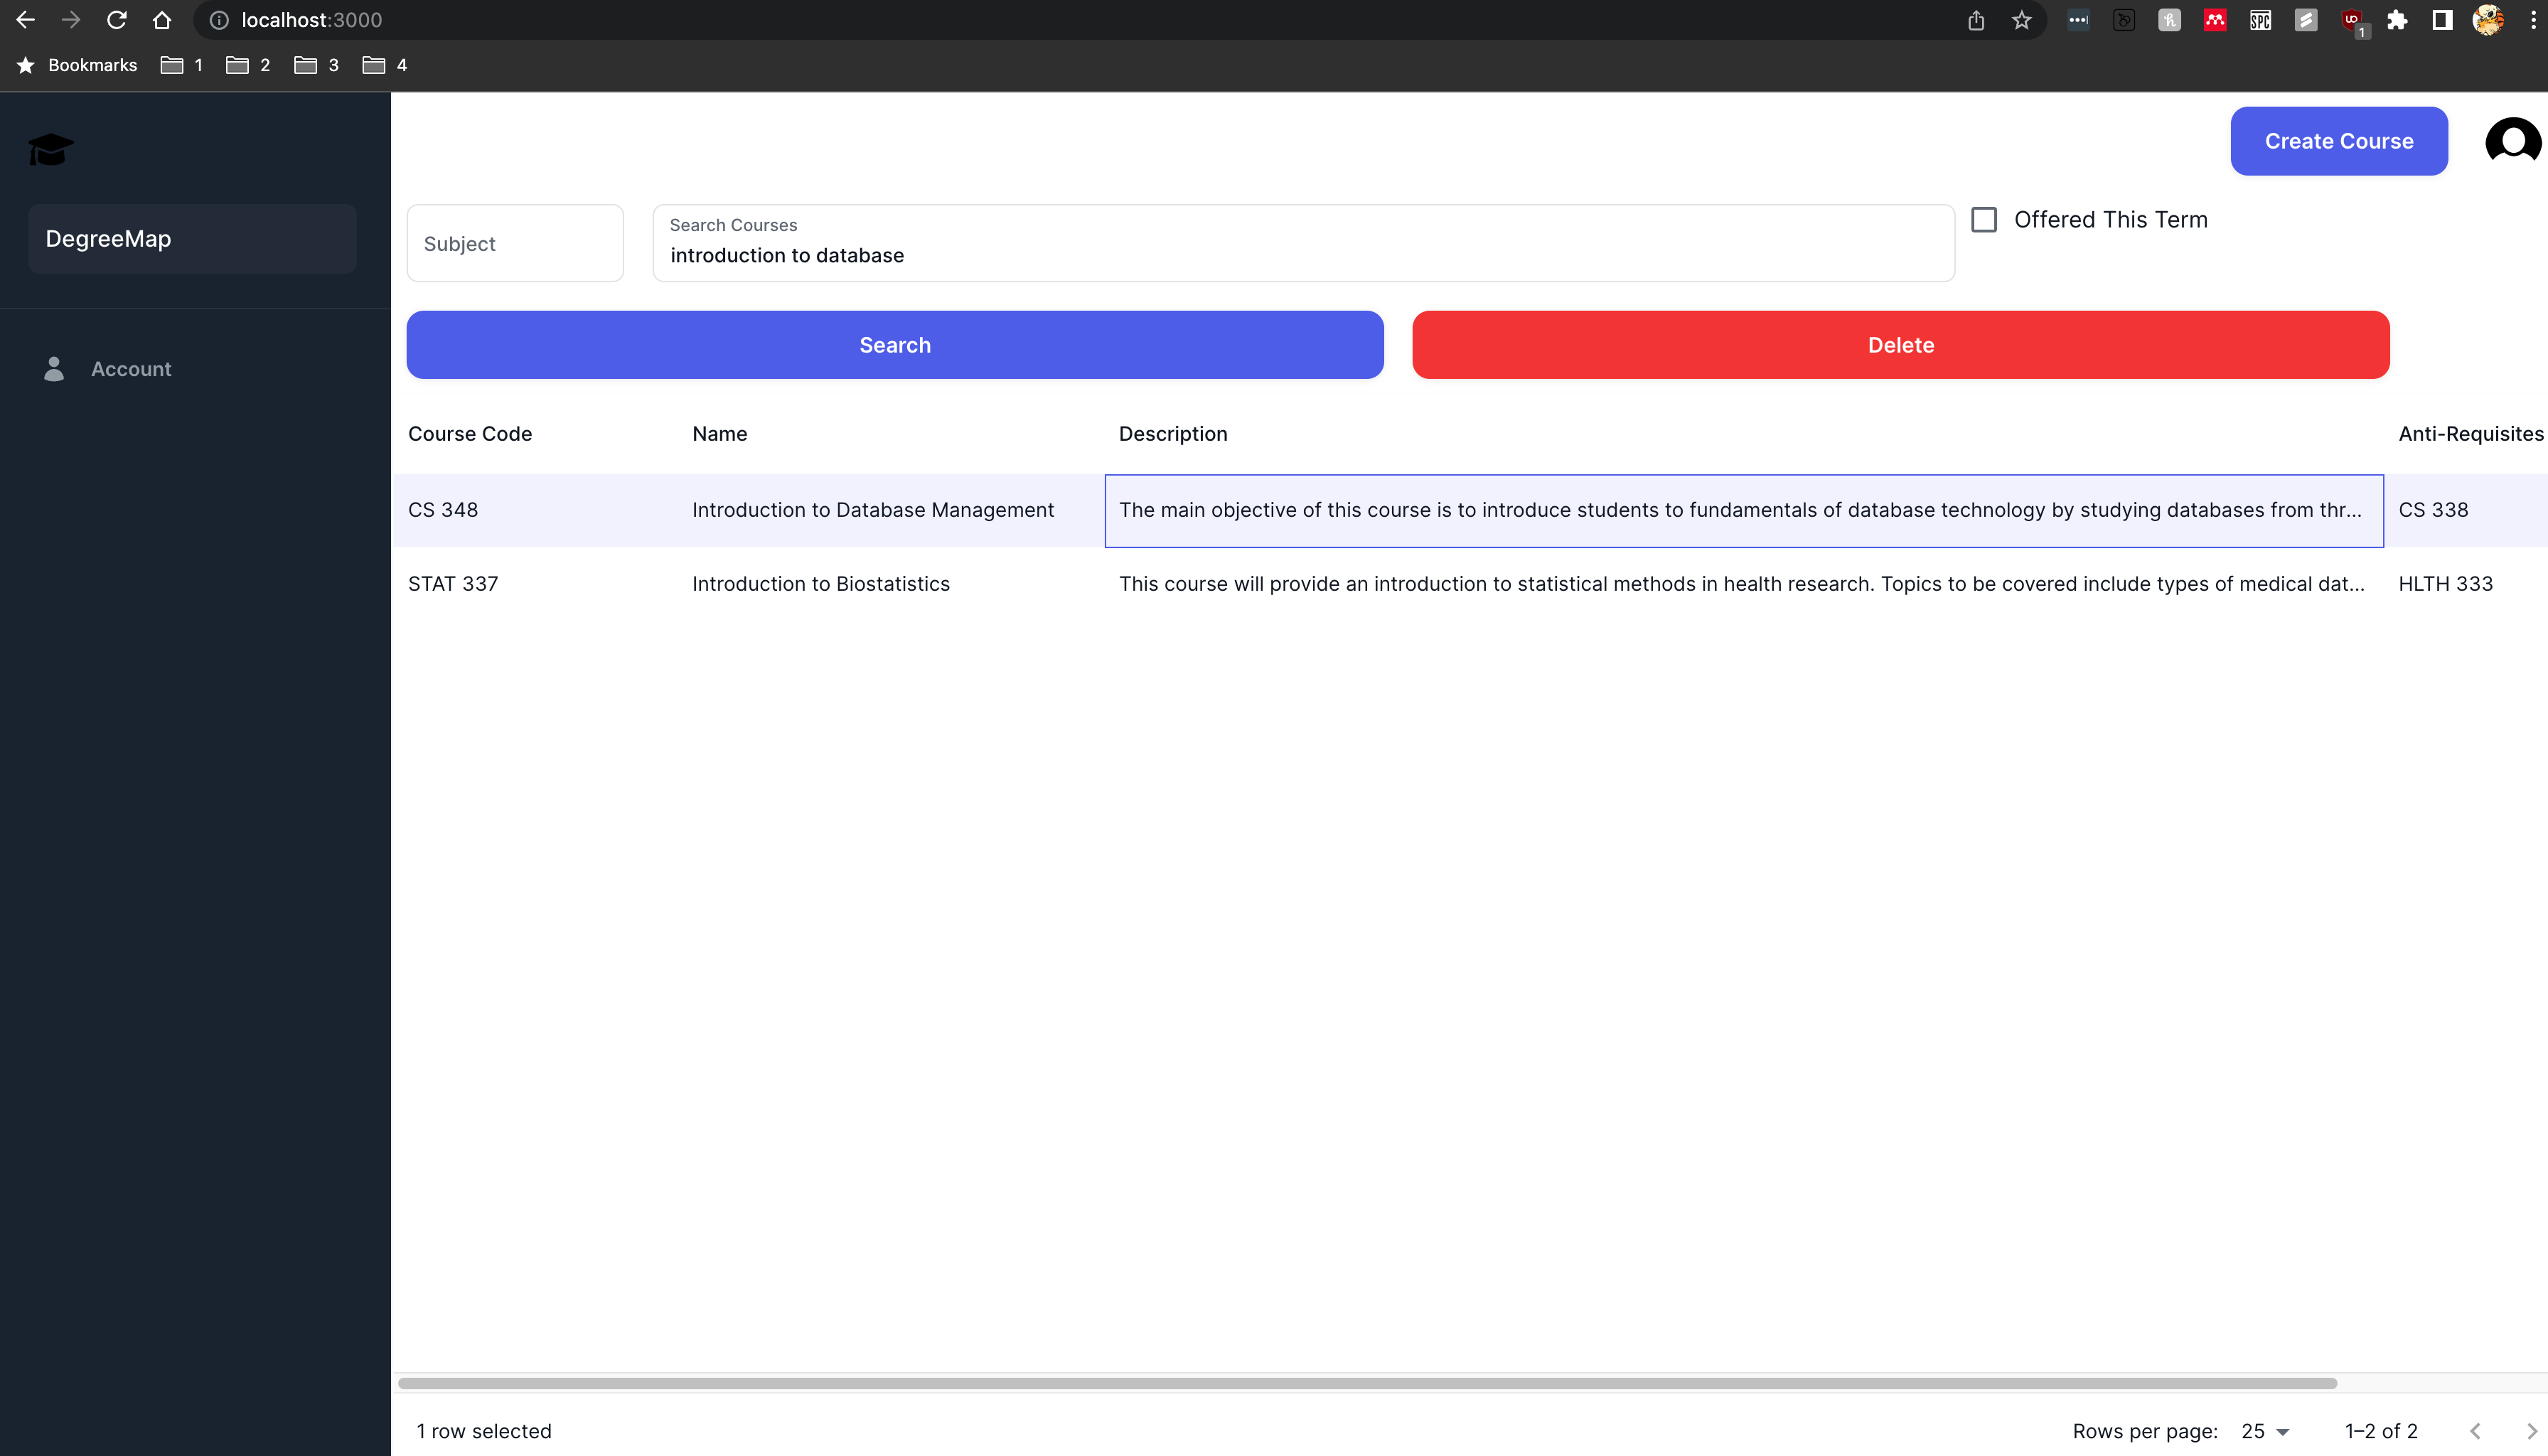
\includegraphics[width=400px]{images/R7/i3}
    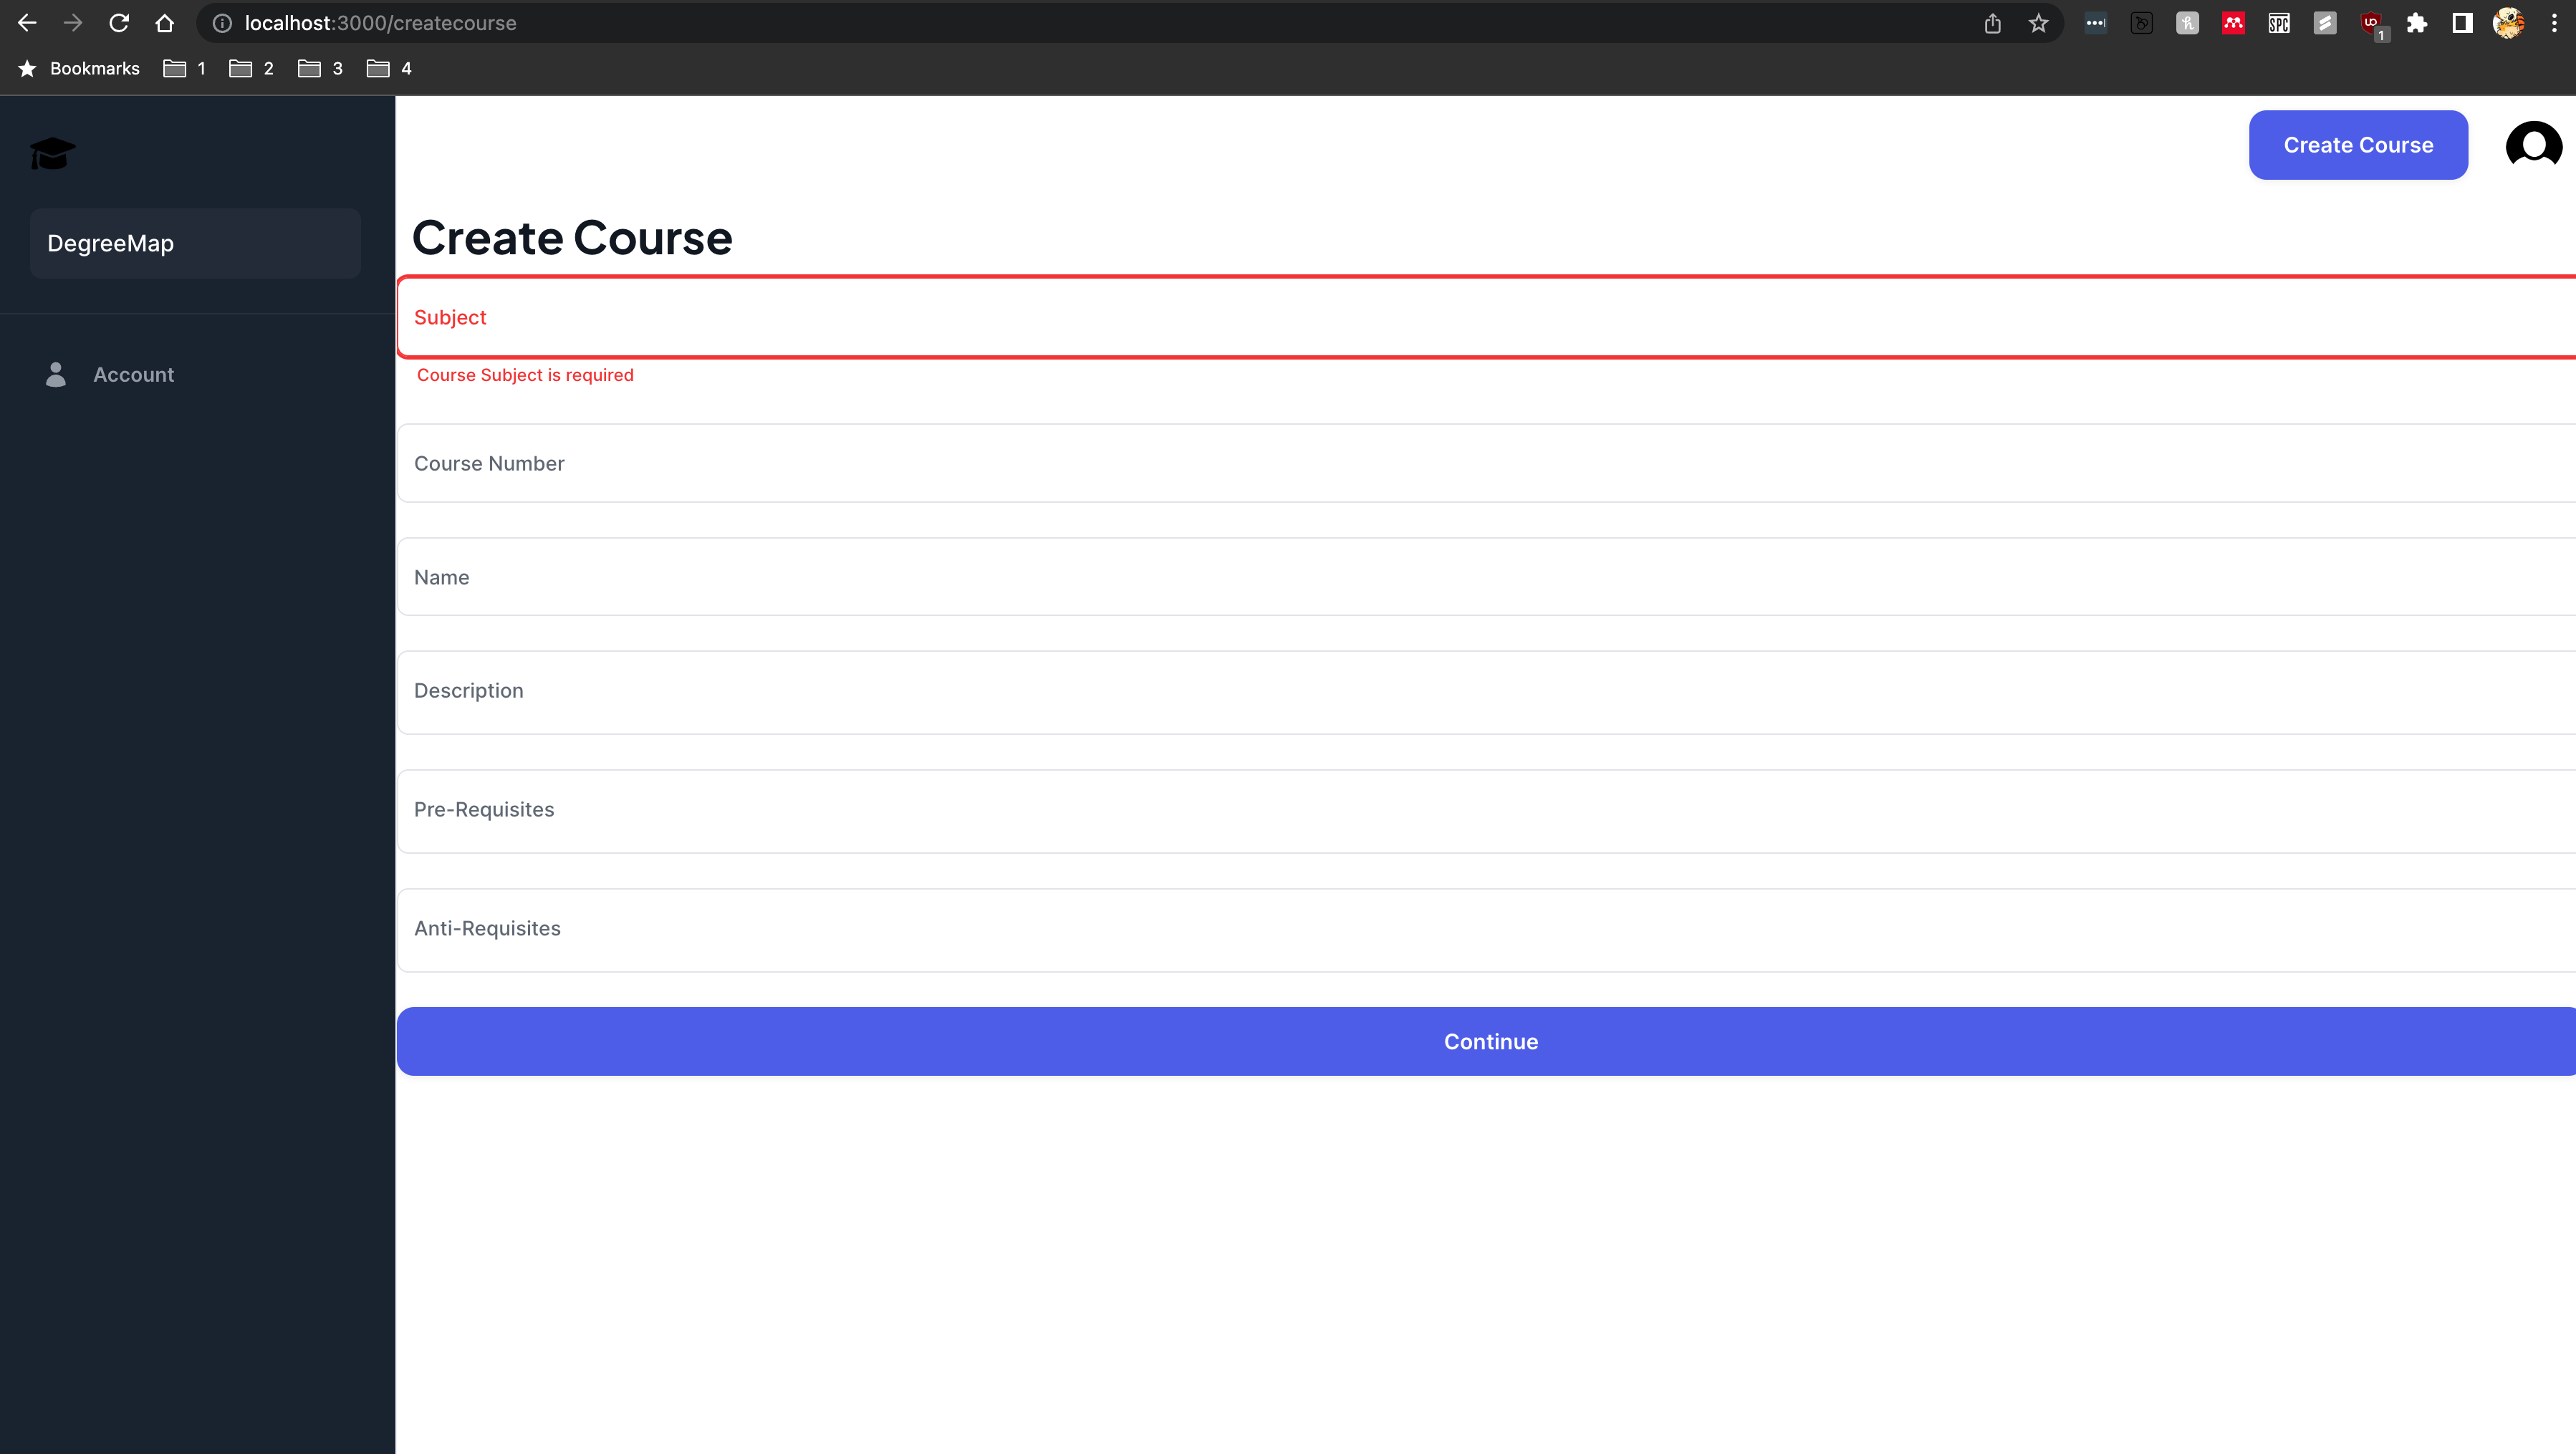
\includegraphics[width=400px]{images/R7/i4}
\end{center}
\subsubsection*{Testing List/Search}
\begin{itemize}
    \item Click the graduation cap in the top left corner if you're not already on the main page.
    \item Try search with a subject that doesn't exist, red text above the search button will appear saying the subject is invalid.
    \item Try search with a search term less than 4 characters, red text in the text box will appear saying to write more text.
    \item Try search with CS and some search term, then click search. The items will get populated in the table
    \item Swipe left and right to see more columns (anti and pre requisites are on the right and slightly cut off in the picture)
    \item Scroll up and down to see all courses
    \item Click 'Offered This Term' and then click search again, fewer courses will appear since those courses don't have any valid sections this term.
\end{itemize}
\subsubsection*{Testing Deleting Courses}
\begin{itemize}
    \item Log in as a regular user and go to the main page.
    \item Do a normal search and click on any row, the delete button will not appear next to the search button.
    \item Log out and then log back in as an admin. Repeat the above point with this account. The delete button will appear this time, click it and see that the entry disappears from the table and the database.
\end{itemize}
\subsubsection*{Testing Creating Courses}
\begin{itemize}
    \item Log in as a regular user and go to the main page.
    \item You will not see a 'Create Course' button in the top right next to the account icon.
    \item Log in as an administrator user and you will see the icon this time, click it. You will be redirected to the create course page
    \item Enter CS and 341, with any information for the other fields. Red text will appear saying the course already exists.
    \item Enter a unique subject and course code, then enter anything for the other fields (valid pre/anti-requisite), then click continue. Green text will appear saying the submission was successful.
    \item Enter a unique subject and course code, but enter an invalid pre-requisite course and and/or an invalid anti-requisite course. Red text will appear saying that the pre/anti-requisite string is invalid.
    \item Double check that the course wasn't inserted if a failure message appears by going to the main page and searching for the course. It will not show up since the insertion would have been cancelled because of the error.
\end{itemize}
\section*{R8. Add User's Student Schedule}
\label{sec:R8}
\subsection*{R8a. Interface Design}
\subsubsection*{View Sections}
This feature is critical to help students manage the course sections that are provided by the university during the term and help them build their schedule for the current term. In the side bar, along with the course list page, the user can also choose the Sections page. This page will allow the student (user) to show all course sections in a list. The information for each section will be the section ID, the section schedule, the location, section type (LEC, LAB, etc), and the course ID that's associated with it. This is very different from the course list since it will require aggregating and grouping the sections together based on the course ID that it's for as well as removing sections that conflict with another section the student is already attending.
\subsubsection*{Attending Section}
In each section entry, there will be a plus icon within the section row. If the student (user) presses the plus icon, it will add to the database that the user is currently attending that course section. The plus icon will become a trashcan icon once the data is successfully added to the database. However, if the user attempts to add a section for a course that they don't satisfy the pre/anti-requisites, the application won't add to the database, instead it will display and error box, indicating that they can't take the section.
\subsubsection*{Removing Sections}
If the user presses the trashcan icon for a section, it will remove the section from their schedule. Since the trashcan icon will only appear if the user is taking the section, they can only remove a section from their schedule that they've already marked as attending.
\subsection*{R8b. SQL Query, Testing With Sample Data}
The test sql file with all of these queries can be viewed here: \underline{\href{https://github.com/Kggupta/DegreeMap/tree/main/Database/Queries/TestSample}{TestSample/R8.sql}}, \underline{\href{https://github.com/Kggupta/DegreeMap/tree/main/Database/Queries/TestSample}{TestSample/R8.out}}. All SQL queries are commented to explain what it does for this feature.

\begin{center}
    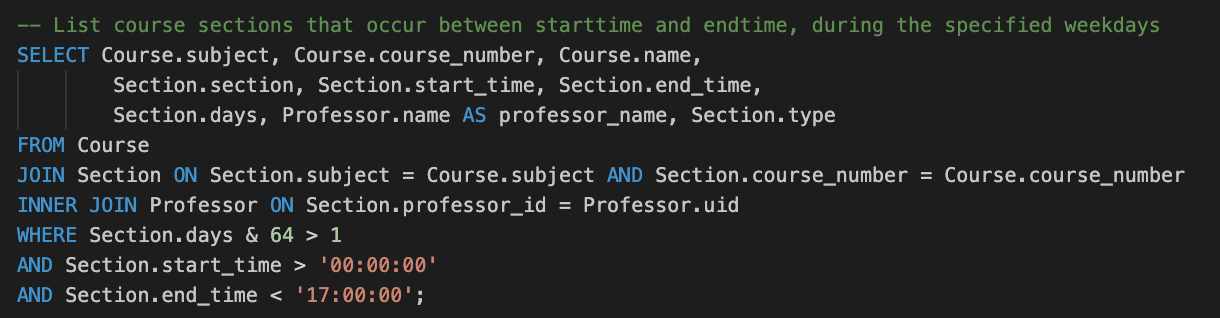
\includegraphics[width=400px]{R8/q1}
    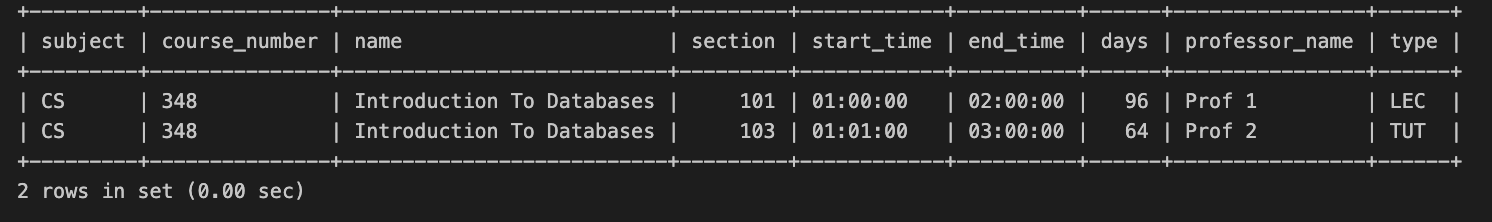
\includegraphics[width=400px]{R8/q1out.png}
\end{center}
First recall that days is stored as an integer, where it's actually a 7 digit binary number where a 1 represents that the course section is offered on that day. Reading from the leftmost binary digit, it starts on Monday.\\

The above query therefore returns all courses and their sections for which it shares at least 1 day with the provided day (in this example, 64 is the same as just Monday) and the section occurs between the provided timings. Essentially, it returns course sections for which it overlaps in some way with the provided day, start, and end values.

\begin{center}
    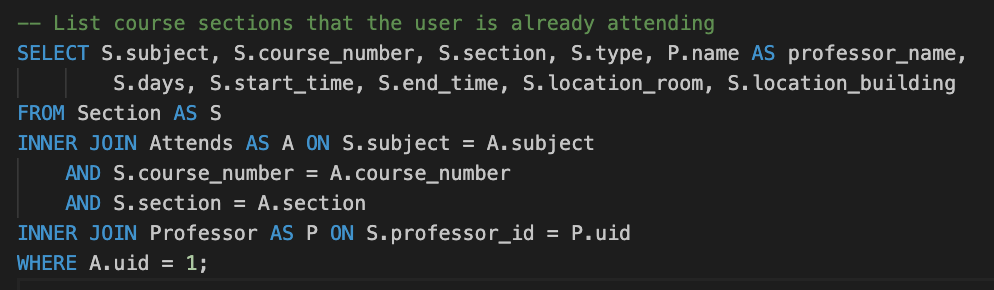
\includegraphics[width=400px]{R8/q2}
    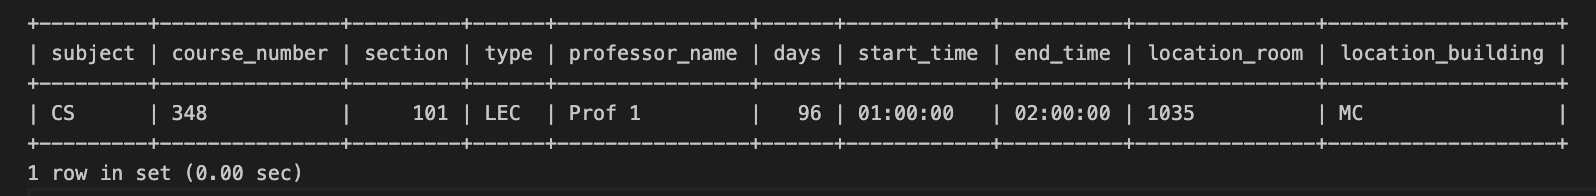
\includegraphics[width=400px]{R8/q2out}
\end{center}
This query returns all the course sections that the user is already attending. User 1 is attending only CS348 in this case which is why that is the only result that appears.\\\\
The client/server would combine the two queries above in JavaScript to get only the courses that don't overlap in terms of scheduled timing with any of the sections the given user is already attending.
\subsection*{R8c. SQL Query, Testing With Production Data}
The test sql file with all of these queries can be viewed here: \underline{\href{https://github.com/Kggupta/DegreeMap/tree/main/Database/Queries/TestProduction}{TestProduction/R8.sql}}, \underline{\href{https://github.com/Kggupta/DegreeMap/tree/main/Database/Queries/TestProduction}{TestProduction/R8.out}}. All SQL queries are commented to explain what it does for this feature.

For this feature, we found that the query for getting sections occurring between start time and end time was running slower on the production database. We noticed that there are two conditions in the query (in above section) that use ranges, specifically start time and end time. Therefore, we created a composite index on these properties to help speed up these range queries. Since insertions on section don't occur, this is an ideal candidate since once the database is populated the first time, we know there's no more insertions on the Section table.
All indexes on the database are stored in \textbf{Database/Queries/CreateIndexes.sql} and get added when the database is populated.

\begin{verbatim}
CREATE INDEX idx_section_time_range ON Section (start_time, end_time);
\end{verbatim}
We tested the performance improvement by first running the same query as in part b, but with the production database. Without the index, we got a result in 1.5sec on average out of 10 runs, but with the index it averaged 0.7sec out of 10 runs. One of these runs is visible in the test production sql files that I attached at the start of this section.
\subsection*{R8d. Implementation, Snapshot, Testing}
Below are screenshots of the implementation for searching for a course to attend, attending a course, and un-attending a course.
\begin{center}
    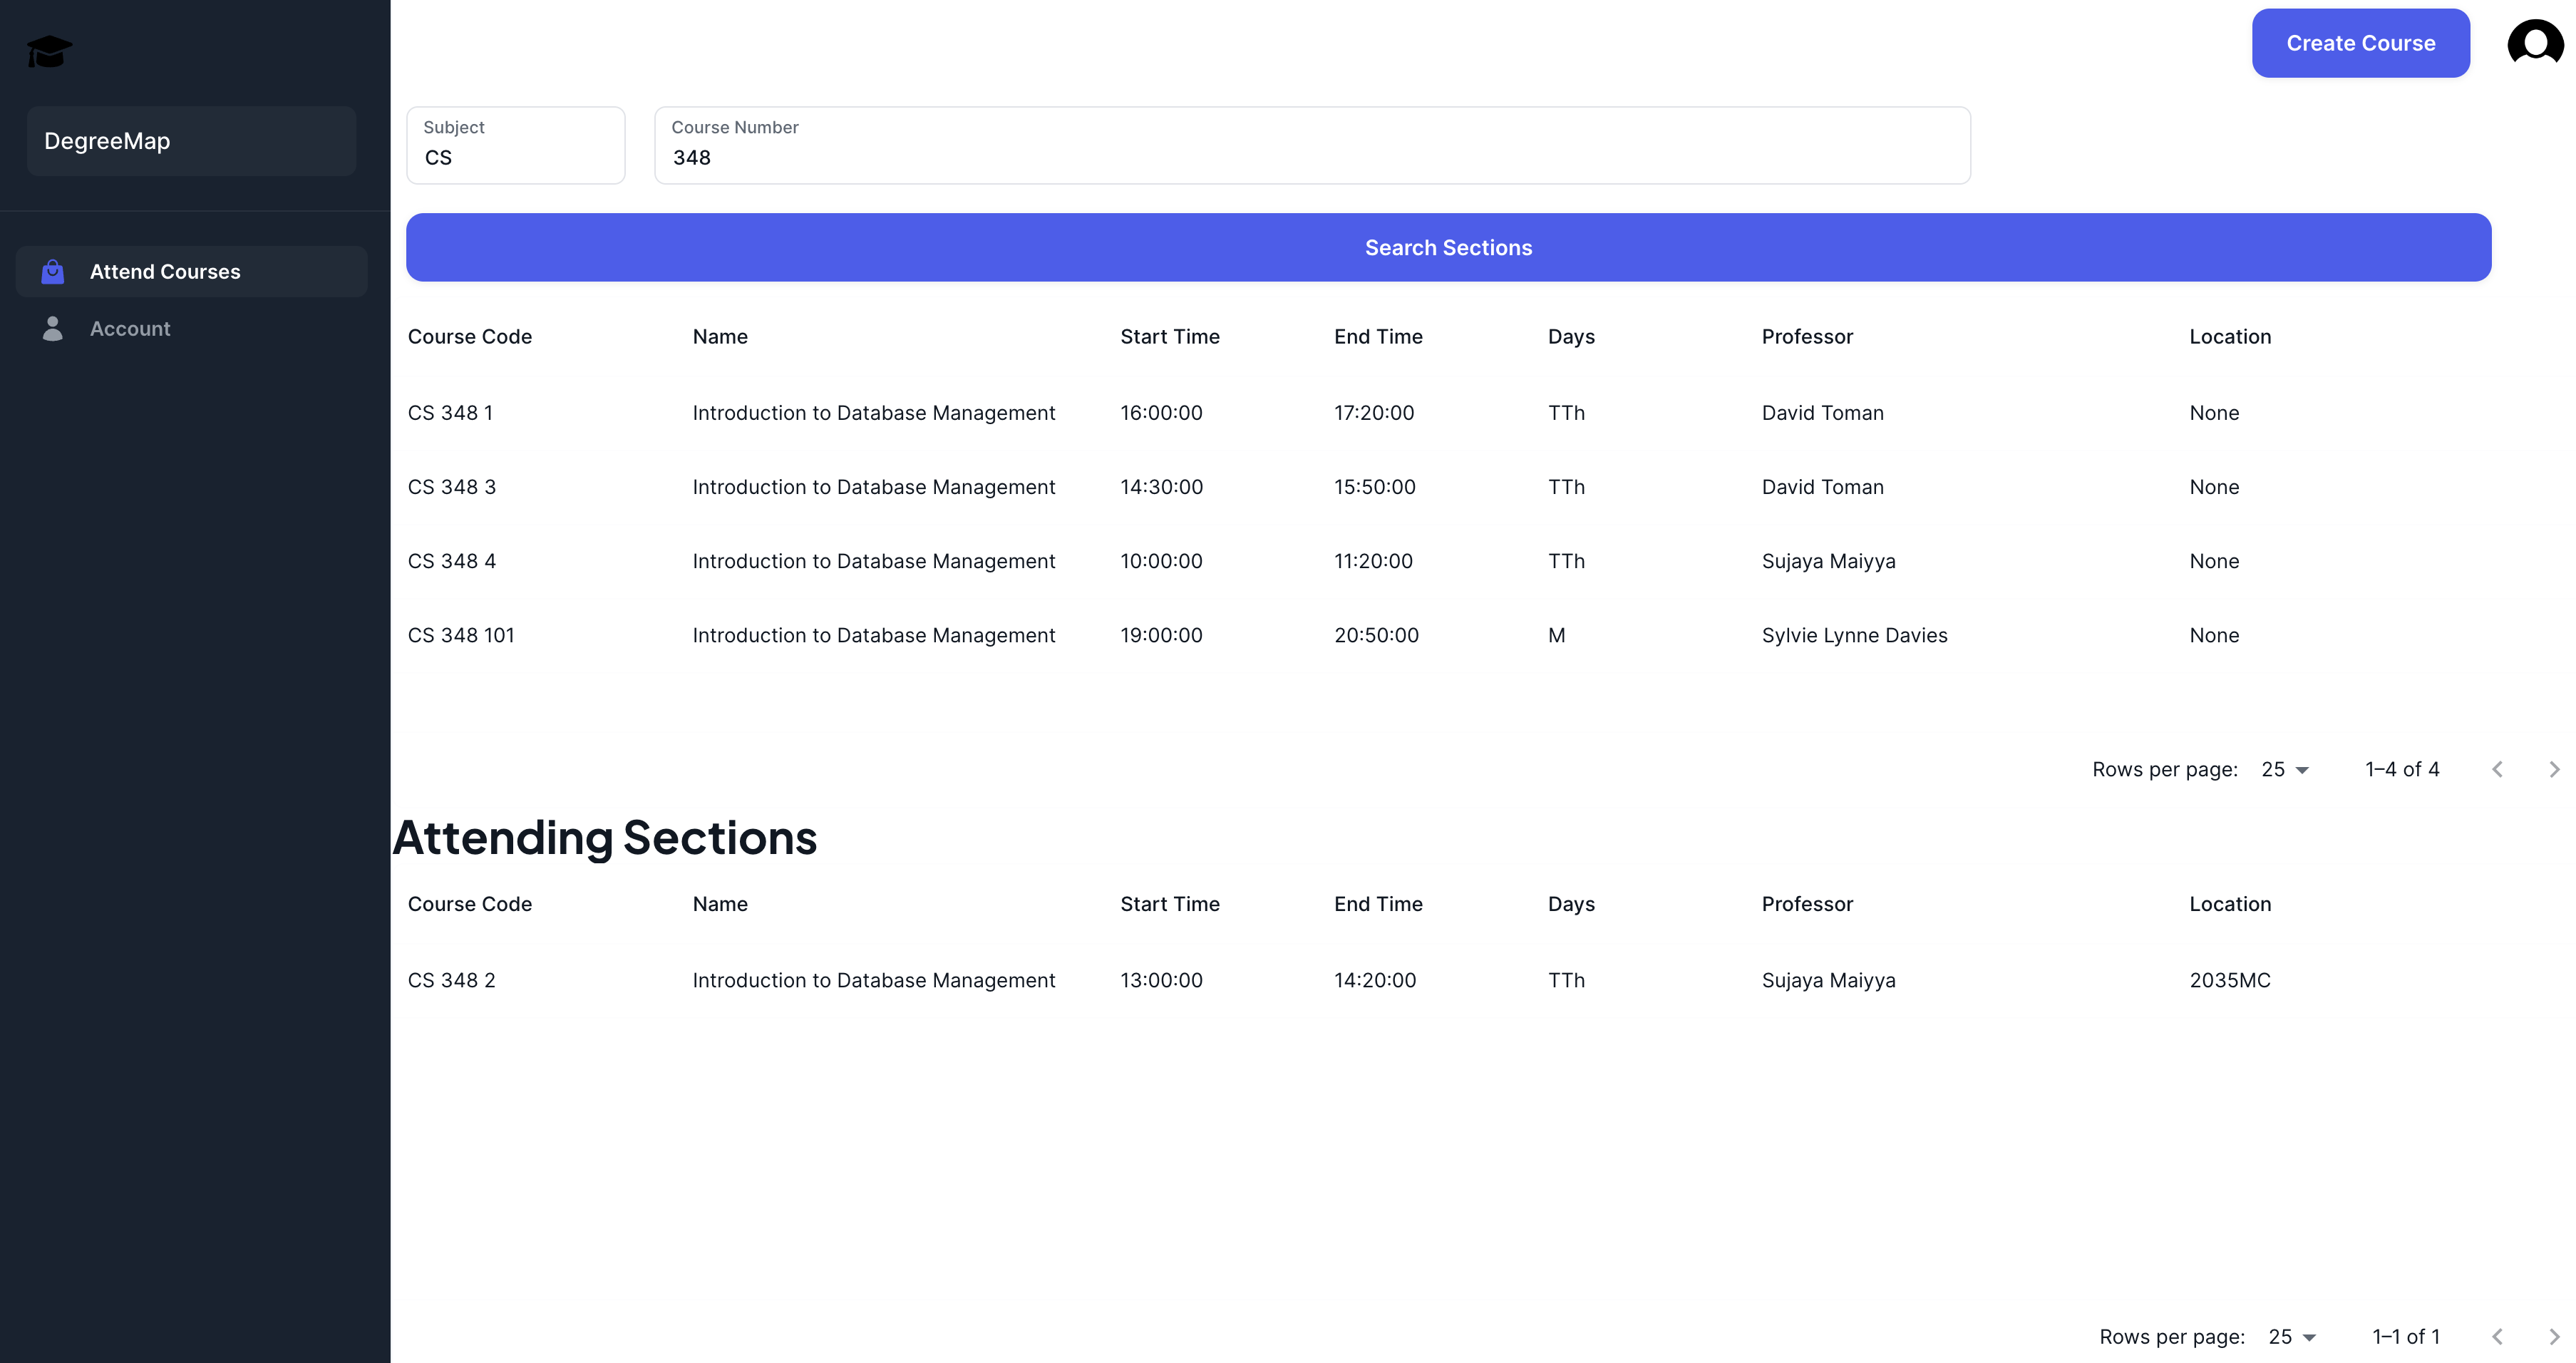
\includegraphics[width=400px]{R8/i1}
    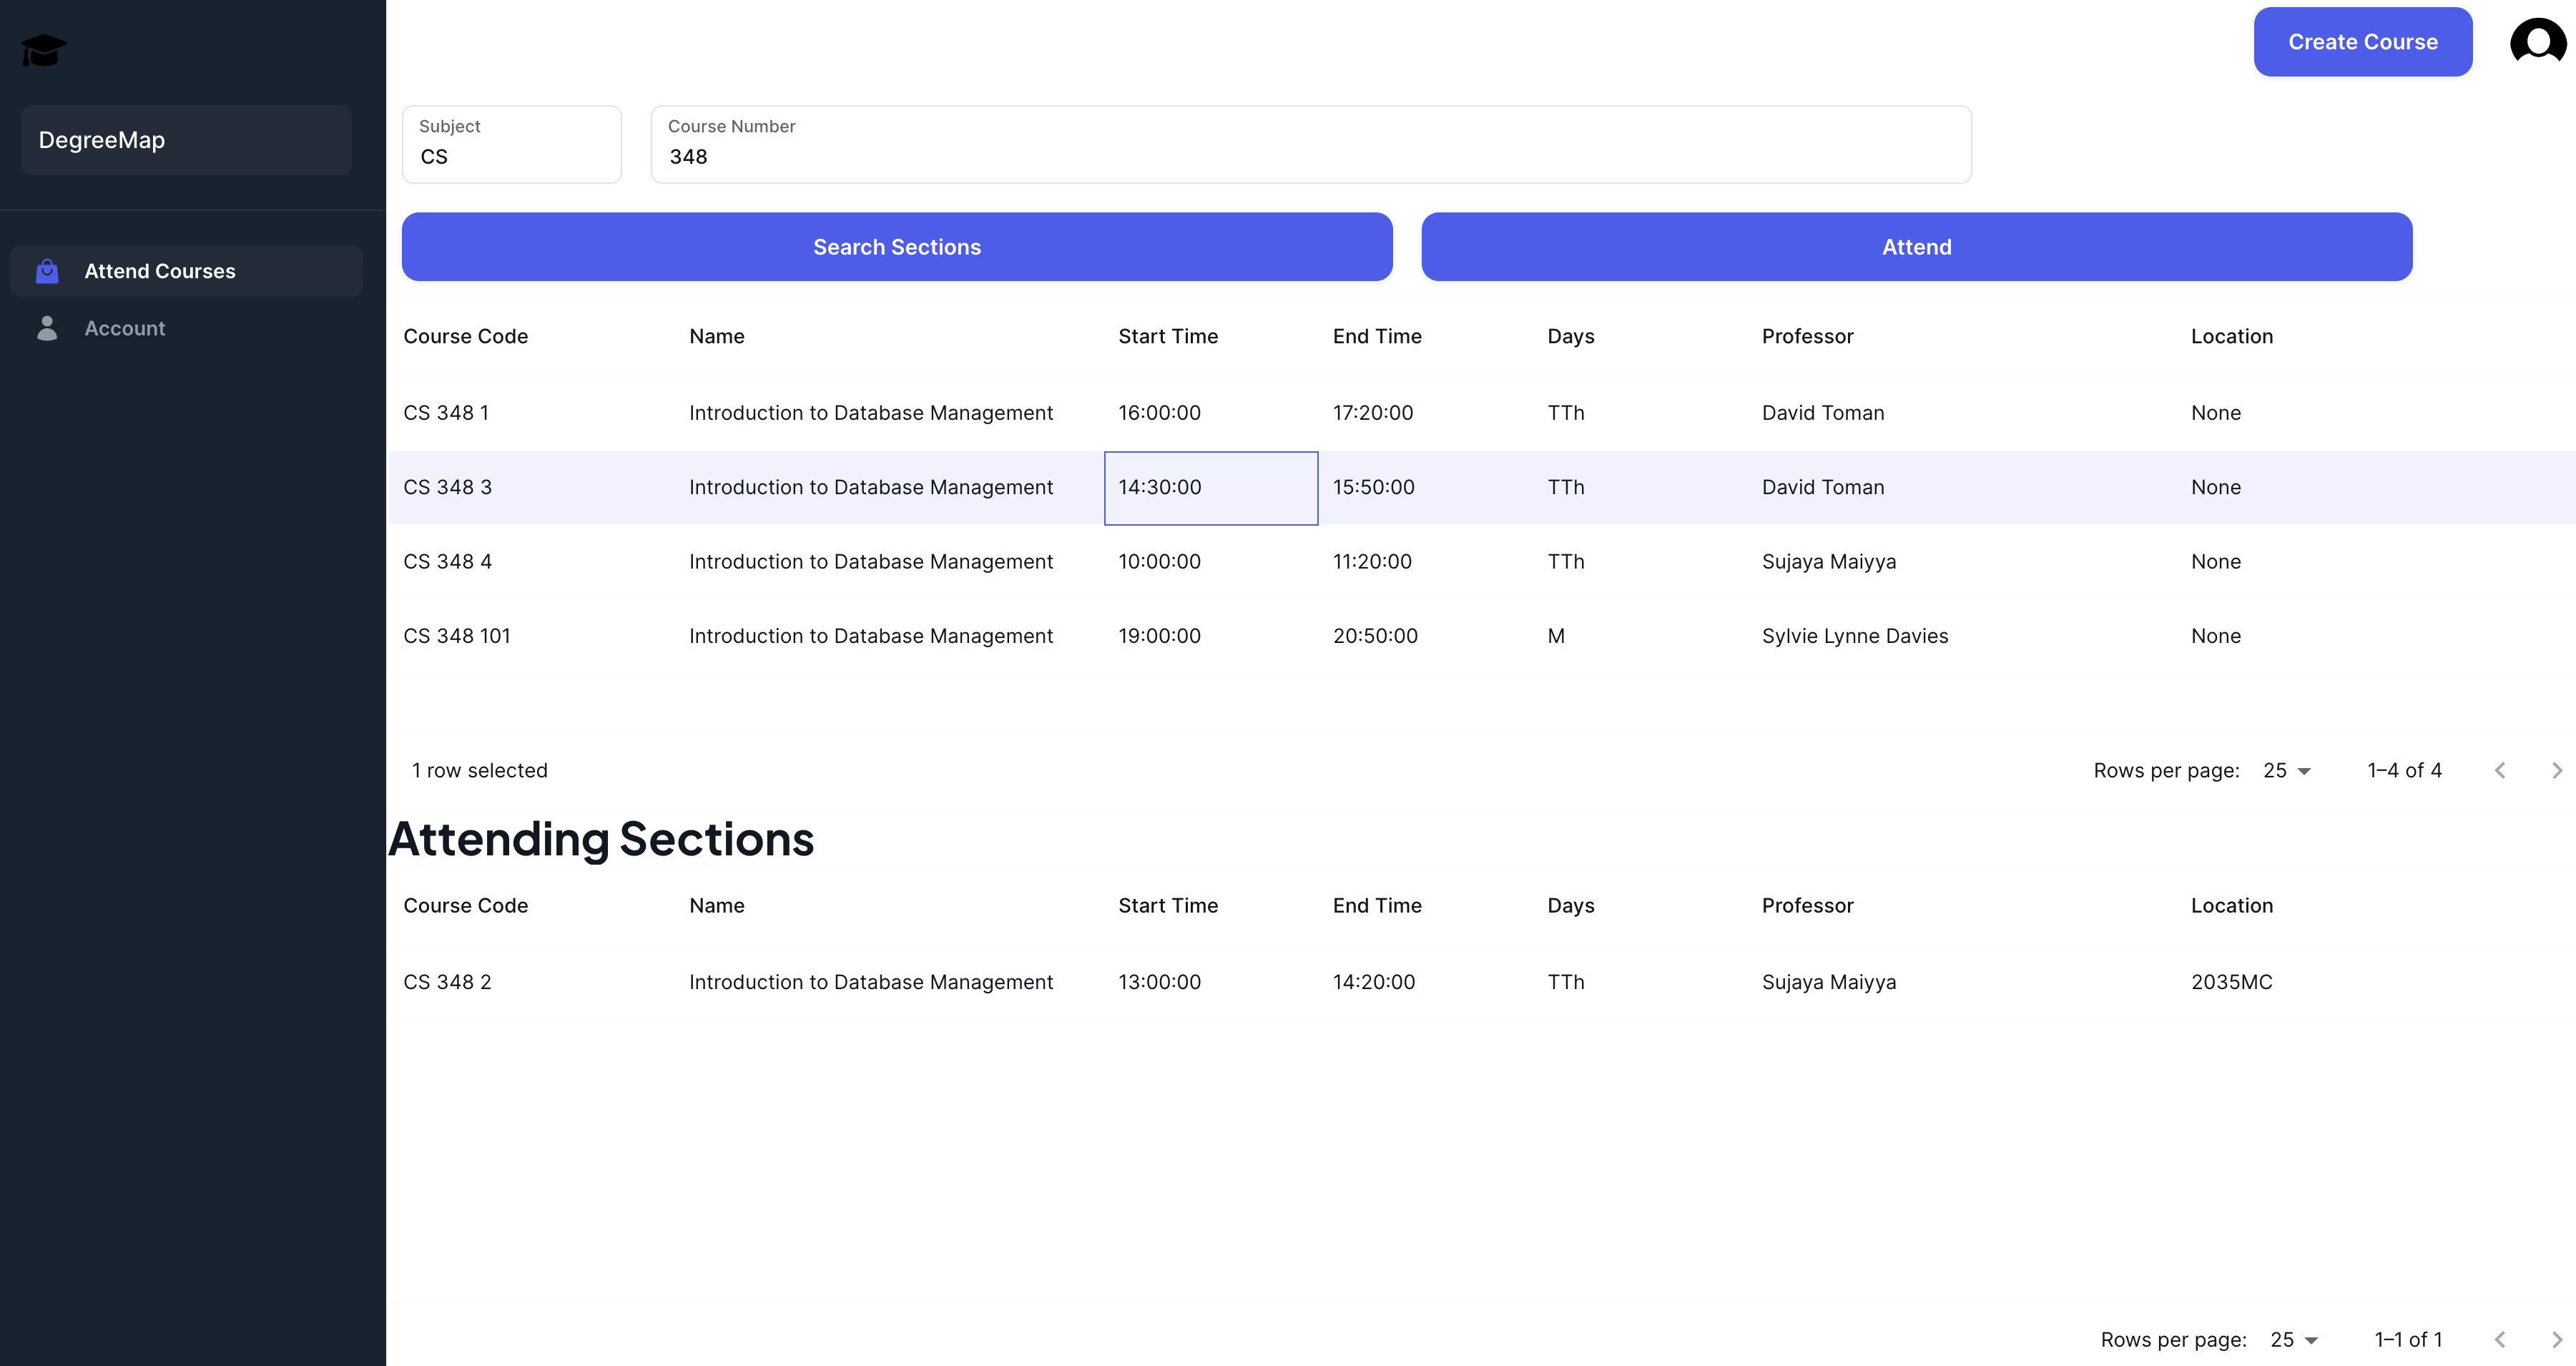
\includegraphics[width=400px]{R8/i2}   
    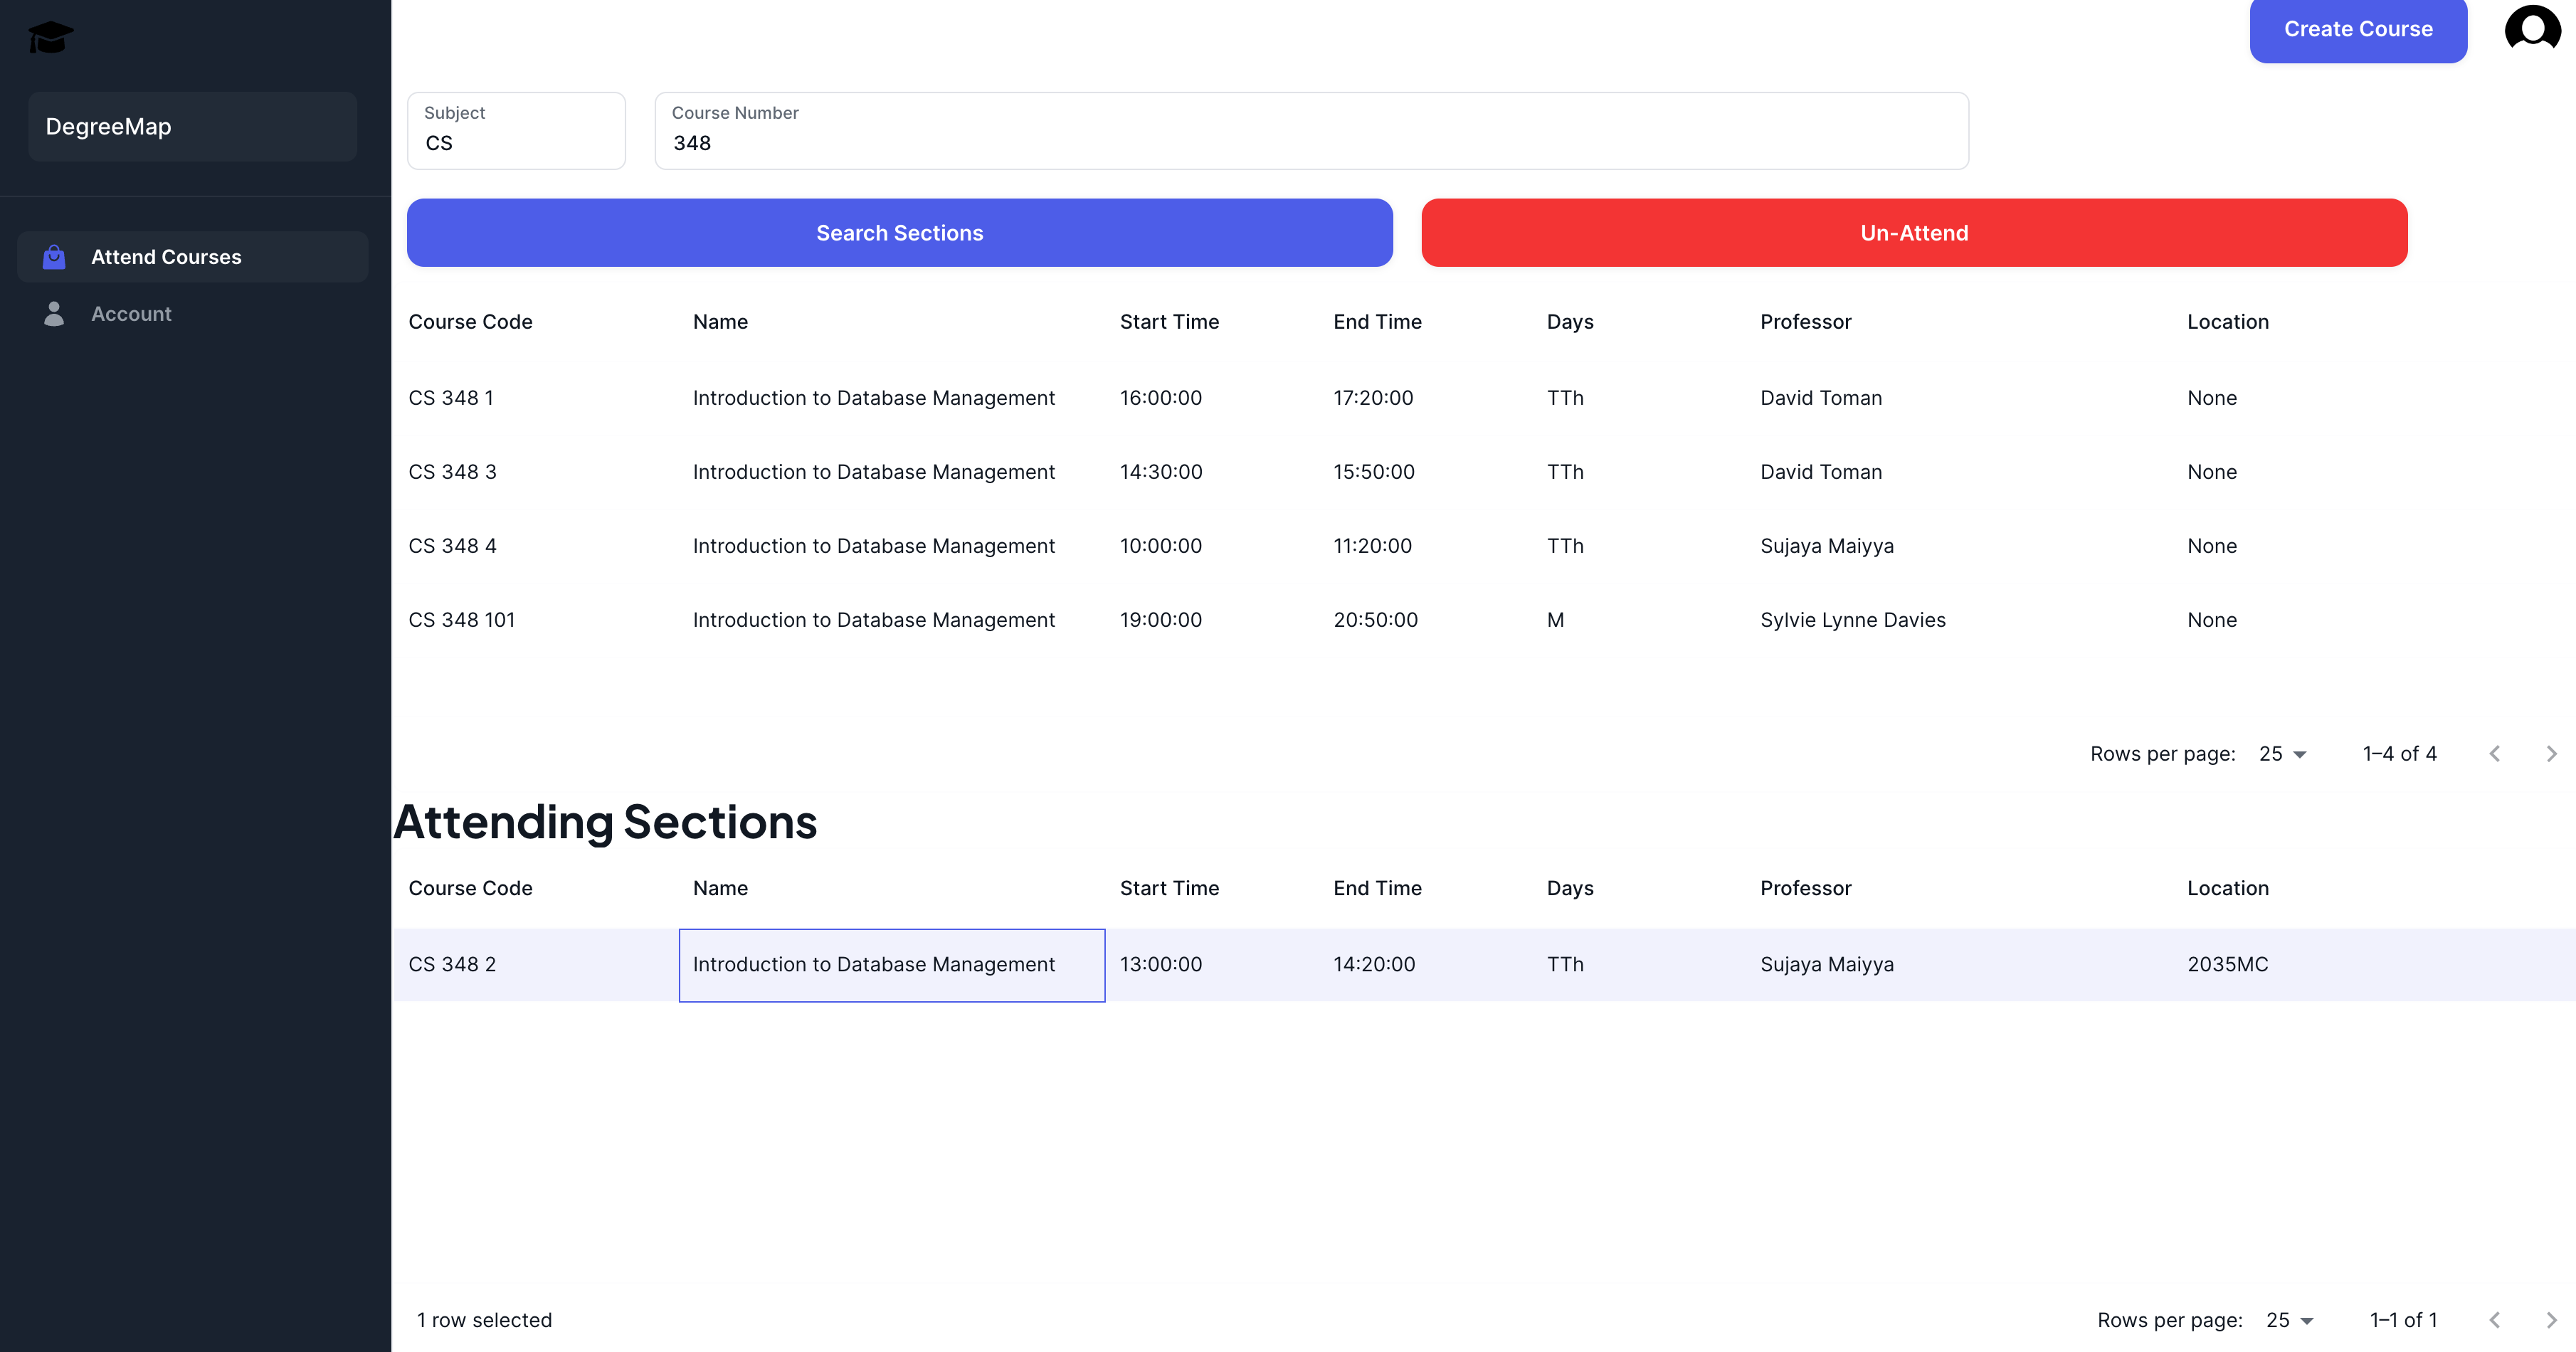
\includegraphics[width=400px]{R8/i3} 
\end{center}
\subsubsection*{Testing Sections Page}
\begin{itemize}
    \item Click the attend courses in the side bar
    \item Search for any course that exists and click search section, the sections will appear in the list
    \item Search for a course that doesn't exist, the search box will remain empty and a error will appear
    \item Select a course in the top table, the attend button will appear, click it and it will be moved to the attending sections table
    \item Select a course in the bottom table, the un-attend button will appear, click it and it will disappear from the attending sections table.
    \item Search for a course that you know has sections overlapping with a section you're already attending. It will not show up in the table.
\end{itemize}
\section*{R9. Manage Friends}
\label{sec:R9}
\subsection*{R9a. Interface Design}
\subsubsection*{List Friends}
This feature is primarily to help students find people that are taking, or have taken the same courses and course sections as them, with the intention that they can more easily make friends and get help for their courses. Another tab in the side bar list, along with course list and sections, is the friends tab. This page lists all the friends that the UW student has, or has been friended by another student, in alphabetical order by name. In each friend entry, there is the name of the friend, their email, a list of courses that you have both taken, a list of course sections that you're both taking together, and an "X" icon button. 
\subsubsection*{Remove Friends}
When a user presses the "X" icon, the application prompts them to cancel or confirm. If the user cancels, the dialogue closes and nothing happens. If the user confirms, the friend is removed from the list and database. 
\subsubsection*{Add Friends}
There is also a search bar at the top of this page where the user can enter the students email and click the "Add Friend" button next to the search bar. If the friend exists in the database, the users aren't already friends, and the email is not the user them self, the friend will be added to the user's list of friends and the same data will become visible for the new friend.
\subsubsection*{Suggest Friends}
The application will also have a separate section at the bottom of the page, after the list of current friends, where there's a list of suggested friends based on them taking one or more identical courses or course sections. It will show the mutual course/section using the course ID next to the friend name and email. The suggestion rows will have a plus icon button in place of the "X" icon, where, if pressed, the friend will be removed from the suggested list of friends and added to the user's current list of friends.
\subsection*{R9b. SQL Query, Testing With Sample Data}
The test sql file with all of these queries can be viewed here: \underline{\href{https://github.com/Kggupta/DegreeMap/tree/main/Database/Queries/TestSample}{TestSample/R9.sql}}, \underline{\href{https://github.com/Kggupta/DegreeMap/tree/main/Database/Queries/TestSample}{TestSample/R9.out}}. All SQL queries are commented to explain what it does for this feature.

\begin{center}
    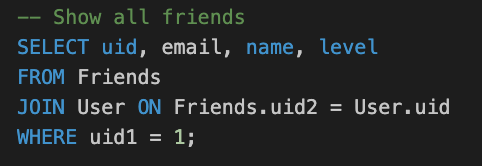
\includegraphics[width=400px]{R9/q1}
    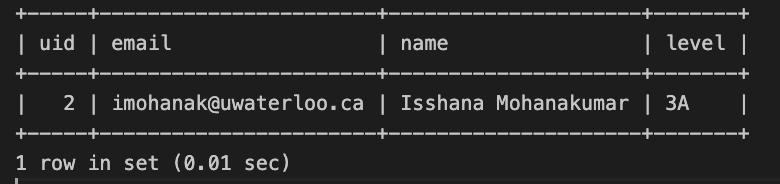
\includegraphics[width=400px]{R9/q1out}
\end{center}
This demonstrates the simple request to get the friend list for a specific user, in this case, user 1 is only friends with user 2.
\begin{center}
    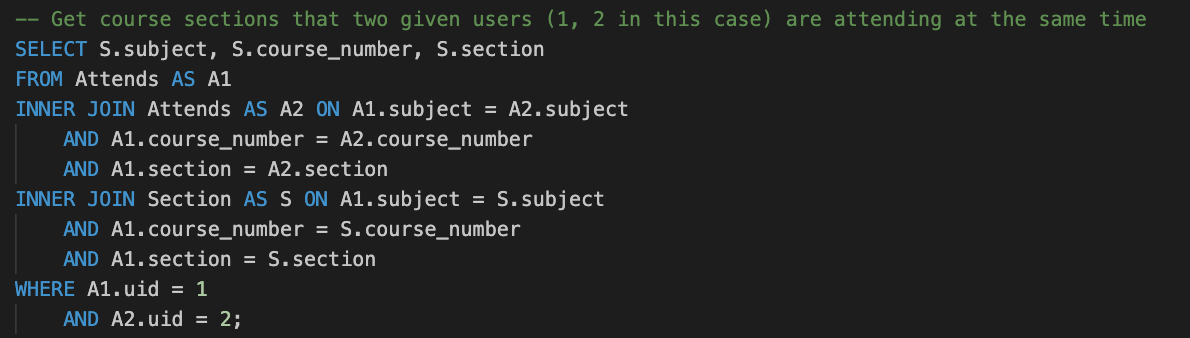
\includegraphics[width=400px]{R9/q2}
    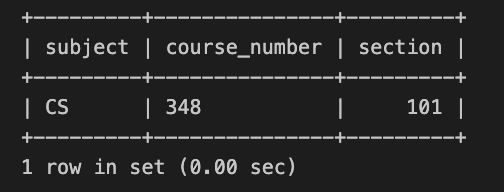
\includegraphics[width=400px]{R9/q2out}
\end{center}
This retrieves all the common course sections between two given users. It combines the attends table twice on the course subject, course number, and section to find users who are taking the same section. In this case, user 1 and user 2 are both taking the same CS348 section. The Section table is also combined so that we can retrieve other section information later, such as location in the production data set.
\begin{center}
    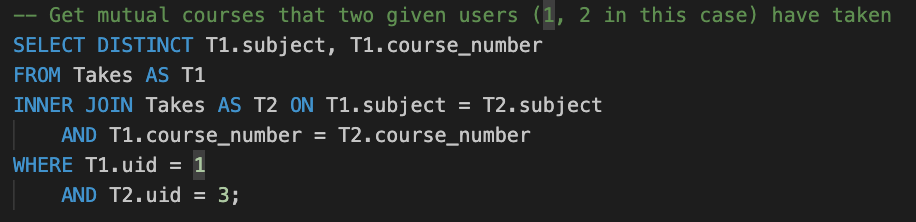
\includegraphics[width=400px]{R9/q3}
    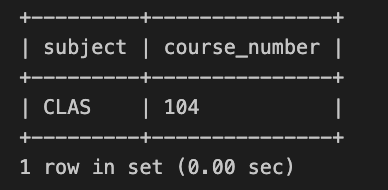
\includegraphics[width=400px]{R9/q3out}
\end{center}
This is just a simple query, similar to the one above that gets all the courses that both users have taken, instead of sections.
\begin{center}
    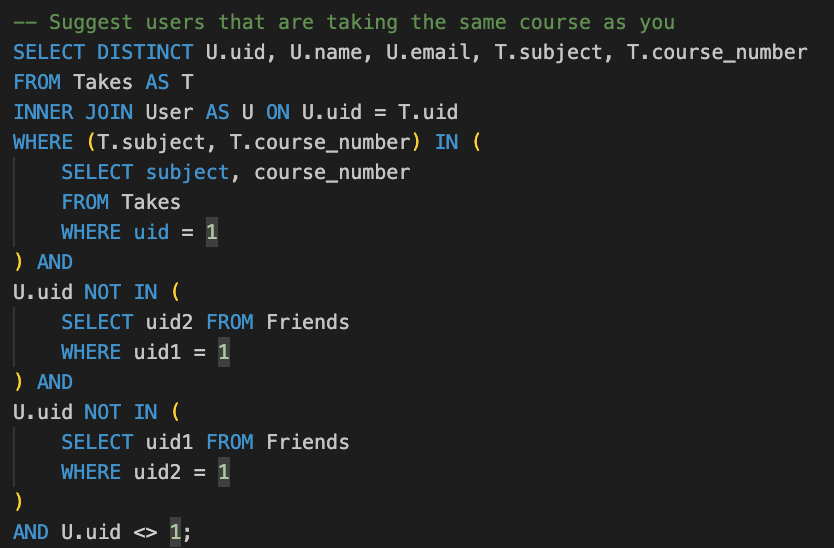
\includegraphics[width=400px]{R9/q4}
    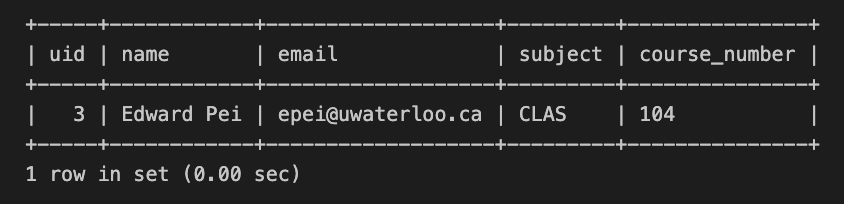
\includegraphics[width=400px]{R9/q4out}
\end{center}
The main part of the feature is the above query that suggests other users who are not already friends that are taking the same courses as you. It gets people who are taking the same courses as you, and then uses two conditions to ensure the user isn't already friends with the specified user. In this case, user 3 took CLAS104 along with user 1 and they're not already friends.
\subsection*{R9c. SQL Query, Testing With Production Data}
The test sql file with all of these queries can be viewed here: \underline{\href{https://github.com/Kggupta/DegreeMap/tree/main/Database/Queries/TestProduction}{TestProduction/R9.sql}}, \underline{\href{https://github.com/Kggupta/DegreeMap/tree/main/Database/Queries/TestProduction}{TestProduction/R9.out}}. All SQL queries are commented to explain what it does for this feature.

This is another case where there are no performance improvements to be made. This is because all queries are based of the primary key. As mentioned before, MySQL by default makes the primary key a clustered index which means that the joins and equality comparisons are all already optimized in terms of indexes. Therefore, there are no performance improvements for this section.
\section*{R10. Manage Courses Taken and Final Grades}
\label{sec:R10}
\subsection*{R10a. Interface Design}
\subsubsection*{Taking A Course}
This feature is valuable for students to keep track of their GPA, the courses they have taken throughout their undergraduate career, and the final grades of each course, since keeping track of it manually is difficult to do and the unofficial transcript only shows the student's average as a percentage rather than a 4.0 scale which is more popular with employers.\\

In the course tab, within each course row, there will also be a plus icon button that, when pressed, will create a pop-up text box, prompting the user to enter their grade in the course. Once they enter a valid grade within (0,100) and the academic level they took the course during, they can press confirm, the popup will disappear and the app will add the course to the database for that user. If the user presses cancel, the popup will disappear and nothing will be added to the database. When a course has already been added, the plus icon will become disabled and greyed out. The application will also check that the user satisfies all the necessary pre/anti-requisites for the course. If they don't, an error box will appear and the information will not be added to the database.
\subsubsection*{View Taken Courses}
On the sidebar list, underneath the manage friend tab, there will be another tab called "Undergraduate Map". In this page, there will be a list of courses that the user has taken grouped by the academic level that it was taken during. For example, CS348, CS349, CS341, CS350, and SPCOM325 could all be grouped under 3A. In each course card, the course ID, and the final grade achieved will be visible. If a course has no grade associated, it will have \textbf{N/A} in place of the grade. In the bottom right of the window, there will be a text field called GPA: X, and cGPA: Y. Where X and Y are calculated based on the courses the student has taken. Courses that don't have a grade, will not affect either GPAs. The application will also show them their rank relative to the other user's cGPAs.
\subsubsection*{Edit Taken Courses}
Within each course card, the user can click on the final grade text box and enter a new valid grade value. If the grade is not valid, an error box will appear and the value won't update. If the value is valid, it's updated in the database and the user's GPAs are re-calculated and updated on the screen as well.
\subsubsection*{Delete Taken Course}
Within each course card, the user can click a trashcan icon button. A confirmation dialogue will open which will ask them to confirm the deletion or cancel. If they cancel, the dialogue closes and nothing else occurs. If they confirm, the dialogue closes and the course entry disappears from the user's Undergraduate Map page and the GPA is recalculated and updated on the page.
\subsection*{R10b. SQL Query, Testing With Sample Data}
The test sql file with all of these queries can be viewed here: \underline{\href{https://github.com/Kggupta/DegreeMap/tree/main/Database/Queries/TestSample}{TestSample/R10.sql}}, \underline{\href{https://github.com/Kggupta/DegreeMap/tree/main/Database/Queries/TestSample}{TestSample/R10.out}}. All SQL queries are commented to explain what it does for this feature.
\begin{center}
    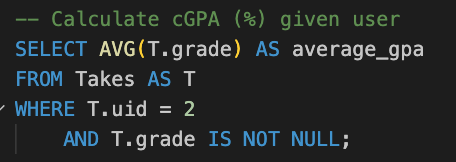
\includegraphics[width=400px]{R10/q1}
    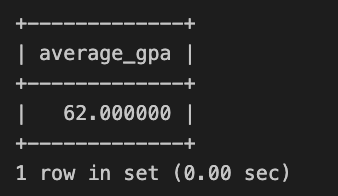
\includegraphics[width=400px]{R10/q1out}
\end{center}
This portion of the feature calculates the specified user's percentage GPA, not including any courses that aren't graded on a percentage basis (NULL).
\begin{center}
    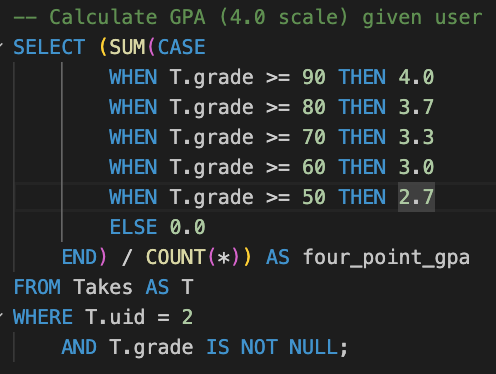
\includegraphics[width=400px]{R10/q2}
    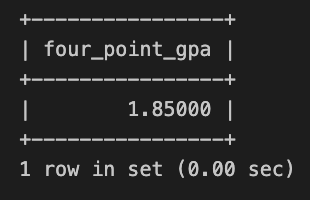
\includegraphics[width=400px]{R10/q2out}
\end{center}
This feature calculates the user's GPA on a 4.0 scale, since this is frustrating for users to do manually as each course needs to be individually converted to the scale, then averaged.
\begin{center}
    \includegraphics[width=400px]{R10/q3}
    \includegraphics[width=400px]{R10/q3out}
\end{center}
This is the main aspect of the feature, it calculates the user's rank with respect to their average percentage GPA, relative to all the other users of the application.\\
This demonstrates all of the features related to users taking courses. The main queries for this feature are calculating GPAs, and showing user rank relative to others.
\subsection*{R10c. SQL Query, Testing With Production Data}
The test sql file with all of these queries can be viewed here: \underline{\href{https://github.com/Kggupta/DegreeMap/tree/main/Database/Queries/TestProduction}{TestProduction/R10.sql}}, \underline{\href{https://github.com/Kggupta/DegreeMap/tree/main/Database/Queries/TestProduction}{TestProduction/R10.out}}. All SQL queries are commented to explain what it does for this feature.

This is a good candidate for an index on grade because of all the aggregate functions that are used such as AVG.
\begin{verbatim}
CREATE INDEX idx_grade ON Takes (grade);
\end{verbatim}

We took several steps to test the performance increase. First, we created ~2000 users and made it so each user takes every course with a random grade out of 100. Then we performed the same query on the user with and without the index. We found that the ranking and GPA calculation queries benefited the most from this index. Where the optimized query took about 1.0sec and the optimized query took 0.6sec on average. An example of one of these runs is visible in the test production file that was attached earlier.
\section*{R11. View Courses Based On Pre/Anti-Requisites}
\label{sec:R11}
\subsection*{R11a. Interface Design}
\subsubsection*{Viewing Available Courses}
This is similar to viewing all the courses (\underline{\hyperref[sec:R7]{R7}}), however, the critical difference is that it automatically considers the courses that the student has already taken to curate the list of courses. This feature is a critical tool for students when planning their courses, since current university provided tools only list pre/anti-requisites and it can be hard to find or remember all the courses a user has previously taken.\\

In the side bar, under the Undergraduate Map tab, there will be a "Plan" tab. In this tab, the user will be able to search for courses based on the subject and course code as well as title, and the application will only present courses that they would be able to take by \textbf{filtering out the ones where they don't satisfy the pre/anti-requisite requirements}. Each course row will have the course ID, title, name, and description. The row will also have a plus icon button in the top right corner of the row.
\subsubsection*{Taking Available Courses}
The plus icon button will show a dialogue box of available sections of the course in a dialogue box and allow the user to select multiple sections, with a limit of one section of each type (LEC, LAB, etc.). Only sections that wouldn't overlap with any course sections that the user is already attending will be shown in the list. The user can press cancel at any time and the dialogue box will close. Once the user has selected the sections they want, has selected at least one section, and presses confirm, the application will close the dialogue box and add those sections to the user's schedule.
\subsection*{R11b. SQL Query, Testing With Sample Data}
The test sql file with all of these queries can be viewed here: \underline{\href{https://github.com/Kggupta/DegreeMap/tree/main/Database/Queries/TestSample}{TestSample/R11.sql}}, \underline{\href{https://github.com/Kggupta/DegreeMap/tree/main/Database/Queries/TestSample}{TestSample/R11.out}}. All SQL queries are commented to explain what it does for this feature.
\begin{center}
    \includegraphics[width=400px]{R11/q1}
    \includegraphics[width=400px]{R11/q1out}
\end{center}
For this feature, the main SQL query that is unique to this feature is getting all the courses that the user satisfies the pre-requisites, hasn't taken any of the anti-requisites and hasn't already taken the course. This query shows how the courses that either don't have pre-requisites or the user has taken the pre-requisistes is selected, then the courses where the user has taken an anti-requisite are removed along with all the courses the user has taken.
\subsection*{R11c. SQL Query, Testing With Production Data}
The test sql file with all of these queries can be viewed here: \underline{\href{https://github.com/Kggupta/DegreeMap/tree/main/Database/Queries/TestProduction}{TestProduction/R11.sql}}, \underline{\href{https://github.com/Kggupta/DegreeMap/tree/main/Database/Queries/TestProduction}{TestProduction/R11.out}}. All SQL queries are commented to explain what it does for this feature.

There are no optimizations to make in this case. This is because all the joins and conditions in this query rely on primary keys which have indexes added by default. The reasoning is the same as earlier features with a similar situation. The primary keys are all composite clustered indexes by default in MySQL, and the queries for this feature are all checking the equality of primary keys, therefore there are no performance improvements to be made for this feature. 
\section*{R12. Visualize Pre-Requisite Graphs}
\label{sec:R12}
\subsection*{R12a. Interface Design}
\subsubsection*{Pre-Requisite Graphs}
Many courses, especially upper year courses, have a very intricate pre-requisite graph that can be really difficult to grasp currently due to the university's scattered web pages that describe each course and the associated pre-requisites. Additionally, these graphs may be several layers deep, spanning from first year to fourth year. Our application will be an invaluable solution for undergraduate students when they're trying to see what's required to take the courses that they're interested in.\\

When a user searches for a course on the home page described in \underline{\hyperref[sec:R7]{R7}}, they can click the icon that looks like three dots connected by lines that is present on each course row. This button will only appear for courses that have a pre-requisite. Once the user clicks this button, they will be directed to a new page where a graph (nodes and un-directed edges) connects the master course they were looking at and the pre-requisites. There could be several layers of pre-requisite courses. The courses that the user has taken will appear in green and the courses that the user has not taken will appear in red.

\subsection*{R12b. SQL Query, Testing With Sample Data}
The test SQL file with all of these queries can be viewed here: \underline{\href{https://github.com/Kggupta/DegreeMap/tree/main/Database/Queries/TestSample}{TestSample/R12.sql}}, \underline{\href{https://github.com/Kggupta/DegreeMap/tree/main/Database/Queries/TestSample}{TestSample/R12.out}}. All SQL queries are commented to explain what it does for this feature.
\begin{center}
    \includegraphics[width=400px]{R12/q1}
    \includegraphics[width=400px]{R12/q1out}
\end{center}
For this feature, it uses a recursive sql query on the PreRequisites table. It starts with the initial query that selects the pre-requisites of the specified course. Then, it recursively joins with the PreRequisites table based on the previous result to fetch additional pre-requisites.
\subsection*{R12c. SQL Query, Testing With Production Data}
The test SQL file with all of these queries can be viewed here: \underline{\href{https://github.com/Kggupta/DegreeMap/tree/main/Database/Queries/TestProduction}{TestProduction/R12.sql}}, \underline{\href{https://github.com/Kggupta/DegreeMap/tree/main/Database/Queries/TestProduction}{TestProduction/R12.out}}. All SQL queries are commented to explain what it does for this feature.

There is no major tuning or changes to the SQL query that can be done for this data in the production database that would increase search performance. The reason why there is no immprovements to be made is because it's a recursive query that hinges solely on primary keys of the pre requisite table. Since MySQL automatically adds indexes for primary keys in tables, there are no further improvements to be made that will increase. performance.Therefore, this section can be considered to be the same as with the sample data.
\section*{R13. AI Course Suggestion Model}
\label{sec:R13}
\subsection*{R13a. Interface Design}
\subsubsection*{Suggesting Courses}
Student's often don't know what course they should take next, using unreliable sources like Reddit and social media to influence their decisions. This feature is built for students by taking the courses they have already taken as documented within the database, and suggesting their next course based on this information. They must take at least 5 courses before this feature will function. The AI model that determines the next course for the student to take will be trained against all the other users in the database using a gradient boost model such as catboost. The model will take five of the most recent courses that the student took and output a course that it suggests for the user which the users should consider taking if they haven't already done so. We will also provide a model for predicting second, and third suggested courses to allow for multiple suggested courses. Within the Undergraduate Map tab, the bottom section of the application window will have a area where it states "Suggested Course" and the course that the AI Model determined the user might enjoy. The suggestion will show the course ID, title, and description. If the users have taken all suggested courses that the AI model suggests, no courses will be shown and this section will be empty.
\subsection*{R13b. SQL Query, Testing With Sample Data}
This feature does not have any significant SQL queries so this section does not apply. The fancy part of this feature is the AI model.
\subsection*{R13c. SQL Query, Testing With Production Data}
This feature does not have any significant SQL queries so this section does not apply. The fancy part of this feature is the AI model.
\section*{R14. Analyse Individual Assignment Grades}
\label{sec:R14}
\subsection*{R14a. Interface Design}
\subsubsection*{Adding Graded Content}
Courses can have many assignments, midterms, exams, and more. This gets difficult for students to manage and determine their estimated grades based on all of the work that's been returned to them already. Therefore, students will be able to get the application to do this analysis for them by adding the graded content for specific courses. From the Undergraduate Map tab, for each course that the user is taking and is graded based on a percentage basis, a icon that looks like a paper will appear in the item. If the user presses this icon, it will go to a new tab where the user can see a list of graded content that's associated with the course. At the end of the list, a button to "Add Content" will be available. When clicked, text boxes for the unique content name, grade, and weight will appear. The name must be an alphanumeric string within 1 to 20 characters. The grade is a non-negative number. The weight is a number between [0, 100], and the sum of all content weights must be within [0,100]. If all the boxes have valid values, the user can press confirm to add the value to the list and database, the estimated grade will be recalculated and updated in the UI. If there are invalid values, the item is not added to the database, the text boxes get cleared and the user is prompted to enter valid information.
\subsubsection*{Removing Graded Content}
In the content list, each item will have a trashcan icon. When pressed, there is a confirmation dialogue. If the user confirms, the content is removed from the database and view, and the estimated maximum and minimum grade is recalculated.
\subsubsection*{Analysing Graded Content}
The view will also show the estimated grade that the user can achieve. The database does all of these calculations.
\subsection*{R14b. SQL Query, Testing With Sample Data}
The test sql file with all of these queries can be viewed here: \underline{\href{https://github.com/Kggupta/DegreeMap/tree/main/Database/Queries/TestSample}{TestSample/R14.sql}}, \underline{\href{https://github.com/Kggupta/DegreeMap/tree/main/Database/Queries/TestSample}{TestSample/R14.out}}. All SQL queries are commented to explain what it does for this feature.

I have not included the queries for inserting and deleting graded content in this report as they are both trivial. They can be seen in the sql files though.

\begin{center}
    \includegraphics[width=400px]{R14/q1}
    \includegraphics[width=400px]{R14/q1_2}
    \begin{verbatim}
+-----------+
| grade     |
+-----------+
| 69.600000 |
+-----------+
1 row in set (0.00 sec)
    \end{verbatim}
\end{center}
This query checks that there exists graded content for the specified user and course. If not, it returns NULL. Otherwise, it takes all of the registered assignment for the given course and their weight and calculates the total estimated grade based on all the given information. In the above case, 69.6 is the correct grade since in the sample data user 1 has the following registered information:
\begin{verbatim}
uid,subject,course_number,name,grade,weight
1,"CS",348,"A1",90,25
1,"CS",348,"A2",91,10
1,"CS",348,"A3",95,40
\end{verbatim}
The manual calculation results in,\\
90*0.25 + 91*0.1 + 95*0.4 = 69.6\\
Which is correct.
\subsection*{R14c. SQL Query, Testing With Production Data}
The test sql file with all of these queries can be viewed here: \underline{\href{https://github.com/Kggupta/DegreeMap/tree/main/Database/Queries/TestProduction}{TestProduction/R14.sql}}, \underline{\href{https://github.com/Kggupta/DegreeMap/tree/main/Database/Queries/TestProduction}{TestProduction/R14.out}}. All SQL queries are commented to explain what it does for this feature.

There is no major tuning or changes to the SQL query that can be done for this data in the production database that would increase search performance. This is because MySQL by default makes the primary key the clustered key, so the entries in the database are clustered based on the key columns that we're looking at such as UID. This means that the aggregations are already optimized.
\section*{R15. SQL Injection Protection And Hashing}
\label{sec:R15}
\subsection*{R15a. Interface Design}
\subsubsection*{SQL Injection Protection}
Database administrators need to be concerned about the security of their applications and associated databases, therefore, having SQL queries that are secure and robust is critical towards building a good application. We can consider the database administrators as the users in this case, but all users, including application users, benefit greatly when their data is secure. The application will be modified so that any section where parameters are inserted into SQL queries are sanitized so that SQL injection can't occur.
\subsubsection*{Password Hashing}
Similarly, storing passwords in plain-text within databases is incredibly insecure. Instead, the authentication algorithms and database will be updated to store the hash of passwords instead of the actual password itself. Additionally, a salt will be added to the end of the passwords to ensure security. 
\subsection*{R15b. SQL Query, Testing With Sample Data}
This feature does not have any significant SQL queries so this section does not apply. SQL injection cleansing and hashing occurs \textbf{BEFORE} the query runs.
\subsection*{R15c. SQL Query, Testing With Production Data}
This feature does not have any significant SQL queries so this section does not apply. SQL injection cleansing and hashing occurs \textbf{BEFORE} the query runs.
\section*{R16. Course Deadline Notifications}
\label{sec:R16}
\subsection*{R16a. Interface Design}
\subsubsection*{Adding Deadlines}
Courses usually have several deadlines that are impossible to keep track of. Students need a way to store all the deadlines associated with their courses and receive notifications when something is approaching. Within the Undergraduate Map tab, each course that the user is taking will have another icon that looks like a calendar. When the calendar is pressed, the application will go to another page. This page lists all of the deadlines associated with the course. There is also an "Add Deadline" button at the end of the list. When this button is pressed, a dialogue box will open that asks for the deadline name and a date+time for when the item is due. The due date must be in the future and within the next four months. The name must be alphanumeric and within 1 to 20 characters. The user can click cancel or confirm. Cancel will close the dialogue. Confirm will add the deadline to the database if all the fields are valid and close the dialogue box. 
\subsubsection*{Removing Deadlines}
The deadlines in the list will have a trashcan icon as well. When clicked, a confirmation dialogue will open where the user can either cancel the change or confirm. If the user confirms, the deadline will be deleted from the database and the confirmation will disappear.
\subsubsection*{Sending Emails}
When the due-date of a deadline exceeds the current time, the application will send an email reminder to the user, including the deadline name and the due-date.
\subsection*{R16b. SQL Query, Testing With Sample Data}
The test sql file with all of these queries can be viewed here: \underline{\href{https://github.com/Kggupta/DegreeMap/tree/main/Database/Queries/TestSample}{TestSample/R16.sql}}, \underline{\href{https://github.com/Kggupta/DegreeMap/tree/main/Database/Queries/TestSample}{TestSample/R16.out}}. All SQL queries are commented to explain what it does for this feature.
\begin{center}
    \includegraphics[width=400px]{R16/q1}
    \begin{verbatim}
Empty set (0.00 sec)
    \end{verbatim}
\end{center}
This just gets the email and deadline information for the deadlines that have passed the current date.
The difficult/fancy part of this feature is the SMTP logic that sends the emails to the user.
\subsection*{R16c. SQL Query, Testing With Production Data}
The test sql file with all of these queries can be viewed here: \underline{\href{https://github.com/Kggupta/DegreeMap/tree/main/Database/Queries/TestProduction}{TestProduction/R16.sql}}, \underline{\href{https://github.com/Kggupta/DegreeMap/tree/main/Database/Queries/TestProduction}{TestProduction/R16.out}}. All SQL queries are commented to explain what it does for this feature.

This is a good opportunity to implement another index since we're doing a range query on due\_date.

\begin{verbatim}
CREATE INDEX idx_deadlines_due_date ON Deadlines (due_date);
\end{verbatim}
This helps because we will almost always be doing the range query as shown in part b for this feature. We measured the performance by adding ~2000 deadlines to the production database and running the query with and without the index. Overall, we found that the non optimized version took on average 0.4sec, while the optimized version took 0.3sec. This difference is very small, but we believe that the improvement is still visible. An instance of one of these runs can be seen in the test production sql files.
\section*{R17. Members}
Everyone contributed equally to the deliverables. We split tasks evenly, with some variance due to different availability of each member.\\

The full list of how the tasks were divided and completed by group members can be seen on the \underline{\href{https://github.com/Kggupta/DegreeMap/blob/main/Members.txt}{GitHub Members.txt}} file.
\section*{C1. README.md}
Our README includes a lot of important information about the application.
\begin{itemize}
    \item \underline{\href{https://github.com/Kggupta/DegreeMap\#degreemap}{Application Description}}
    \item \underline{\href{https://github.com/Kggupta/DegreeMap\#2-create-a-local-instance-of-the-database}{System Setup}}
    \item \underline{\href{https://github.com/Kggupta/DegreeMap\#3-populate-database}{Database Creation}}
    \item \underline{\href{https://github.com/Kggupta/DegreeMap\#31-sample}{Create/Load Sample Data}}
    \item \underline{\href{https://github.com/Kggupta/DegreeMap\#32-production}{Create/Load Production Data}}
    \item \underline{\href{https://github.com/Kggupta/DegreeMap\#4-running-the-application}{Starting The Application}}
    \item \underline{\href{https://github.com/Kggupta/DegreeMap\#41-running-the-client}{Starting Front-end}}
    \item \underline{\href{https://github.com/Kggupta/DegreeMap\#42-running-the-server}{Starting Back-end}}
    \item \underline{\href{https://github.com/Kggupta/DegreeMap\#5-current-features}{Current Features}}
\end{itemize}


\section*{C2. SQL Code}
There are several SQL scripts to help with all the database operations.

\begin{itemize}
    \item \underline{\href{https://github.com/Kggupta/DegreeMap/blob/main/Database/Queries/CreateDatabase.sql}{Create Database}} - Drop, Create, then Use DegreeMap database
    \item \underline{\href{https://github.com/Kggupta/DegreeMap/blob/main/Database/Queries/CreateTables.sql}{Create Tables}} - Create all tables
    \item \underline{\href{https://github.com/Kggupta/DegreeMap/blob/main/Database/Queries/CreateIndexes.sql}{Create Indexes}} - Create all indexes

    \item \underline{\href{https://github.com/Kggupta/DegreeMap/blob/main/Database/Queries/CreateTriggers.sql}{Create Triggers}} - Create all database triggers
    \item \underline{\href{https://github.com/Kggupta/DegreeMap/blob/main/Database/Queries/DropTables.sql}{Drop Tables}} - Drop all tables
    \item \underline{\href{https://github.com/Kggupta/DegreeMap/blob/main/Database/Queries/Procedures.sql}{Create Procedures}} - Creates all procedures
\end{itemize}
\section*{C3. SQL Queries For Sample Features}
The SQL queries for the sample data are all available in the \underline{\href{https://github.com/Kggupta/DegreeMap/tree/main/Database/Queries/TestSample}{Database/Queries/TestSample}} directory. They are grouped based on which feature they belong to (RX.sql and RX.out).
\section*{C4. SQL Queries For Production Features}
The SQL queries for the production data are all available in the \underline{\href{https://github.com/Kggupta/DegreeMap/tree/main/Database/Queries/TestProduction}{Database/Queries/TestProduction}} directory. They are grouped based on which feature they belong to (RX.sql and RX.out).
\section*{C5. Application Code}
All code is available in the GitHub repository: \underline{\href{https://github.com/Kggupta/DegreeMap}{DegreeMap}}

\end{document}